\PassOptionsToPackage{table}{xcolor} % For \cellcolor in tables
\documentclass[xcolor={usenames}]{beamer}

\usetheme{metropolis}           % Use metropolis theme

\bibliographystyle{apalike}

%%%%%%%%%%%%%%%% Colors
\definecolor{mTableAlert}{HTML}{ED8F34}
\definecolor{mLightGray}{gray}{0.9}

%%%%%%%%%%%%%%%% Packages
\usepackage{tikz} % TikZ
	\usetikzlibrary{decorations.pathreplacing}
	\usetikzlibrary{fadings}
	\usetikzlibrary{positioning}
	\usetikzlibrary{calc}
	\usetikzlibrary{fit}
	\usetikzlibrary{shapes}
	\usetikzlibrary{snakes}
	\usetikzlibrary{arrows}

\usepackage{pgfplots} % PGFPlots
	\pgfplotsset{compat=1.13}
\usepackage{siunitx}

%%%%%%%%%%%%%%%% Data
\begin{filecontents}{first-samples.dat}
	 6  0
	 4 -4
	 1  0
	 8  7
	-3 -3
\end{filecontents}
		
\begin{filecontents}{second-samples.dat}
	 1  8
	-1  5
	-6  0
	-3  4
\end{filecontents}

%%%%%%%%%%%%%%%% First page
\title{Supervised Learning of Neural Random-Access Machines with Differential Evolution}
\date{\today}
\author{Valerio Belli}
\institute{Università degli Studi di Perugia}
\titlegraphic{\hfill
\includegraphics[height=1.5cm]{logo.png}}

\begin{document}
  \maketitle
  \section{Neural Random-Access Machines}
  \begin{frame}{What is?}
	It is a machine introduced in \cite{NRAM:2016} based on a neural network which is capable of manipulating pointers and dereferencing them through ``logical'' circuits. Its objective is to solve a task on which it has been trained creating and executing those circuits.
  \end{frame}
  \begin{frame}{Introduction}
  	Let $N = \{ 1, \dots, I - 1 \}$, where $I$ is an integer constant, the integers set over the NRAM should work. Since the training in \cite{NRAM:2016} is made through a gradient descent algorithm, the NRAM does not work directly over N but over stochastically independent probability distributions, defined as $p \in \mathbb{R}^{I}$ satisfying $0 \leq p_i \leq 1$ and $\sum\limits_{i=0}^{I - 1} p_i = 1$. Moreover, let $T$ the maximum number of timestep of execution of the NRAM.
  \end{frame}
  \begin{frame}{Registers only version}
  	\begin{figure}
  		\centering
  		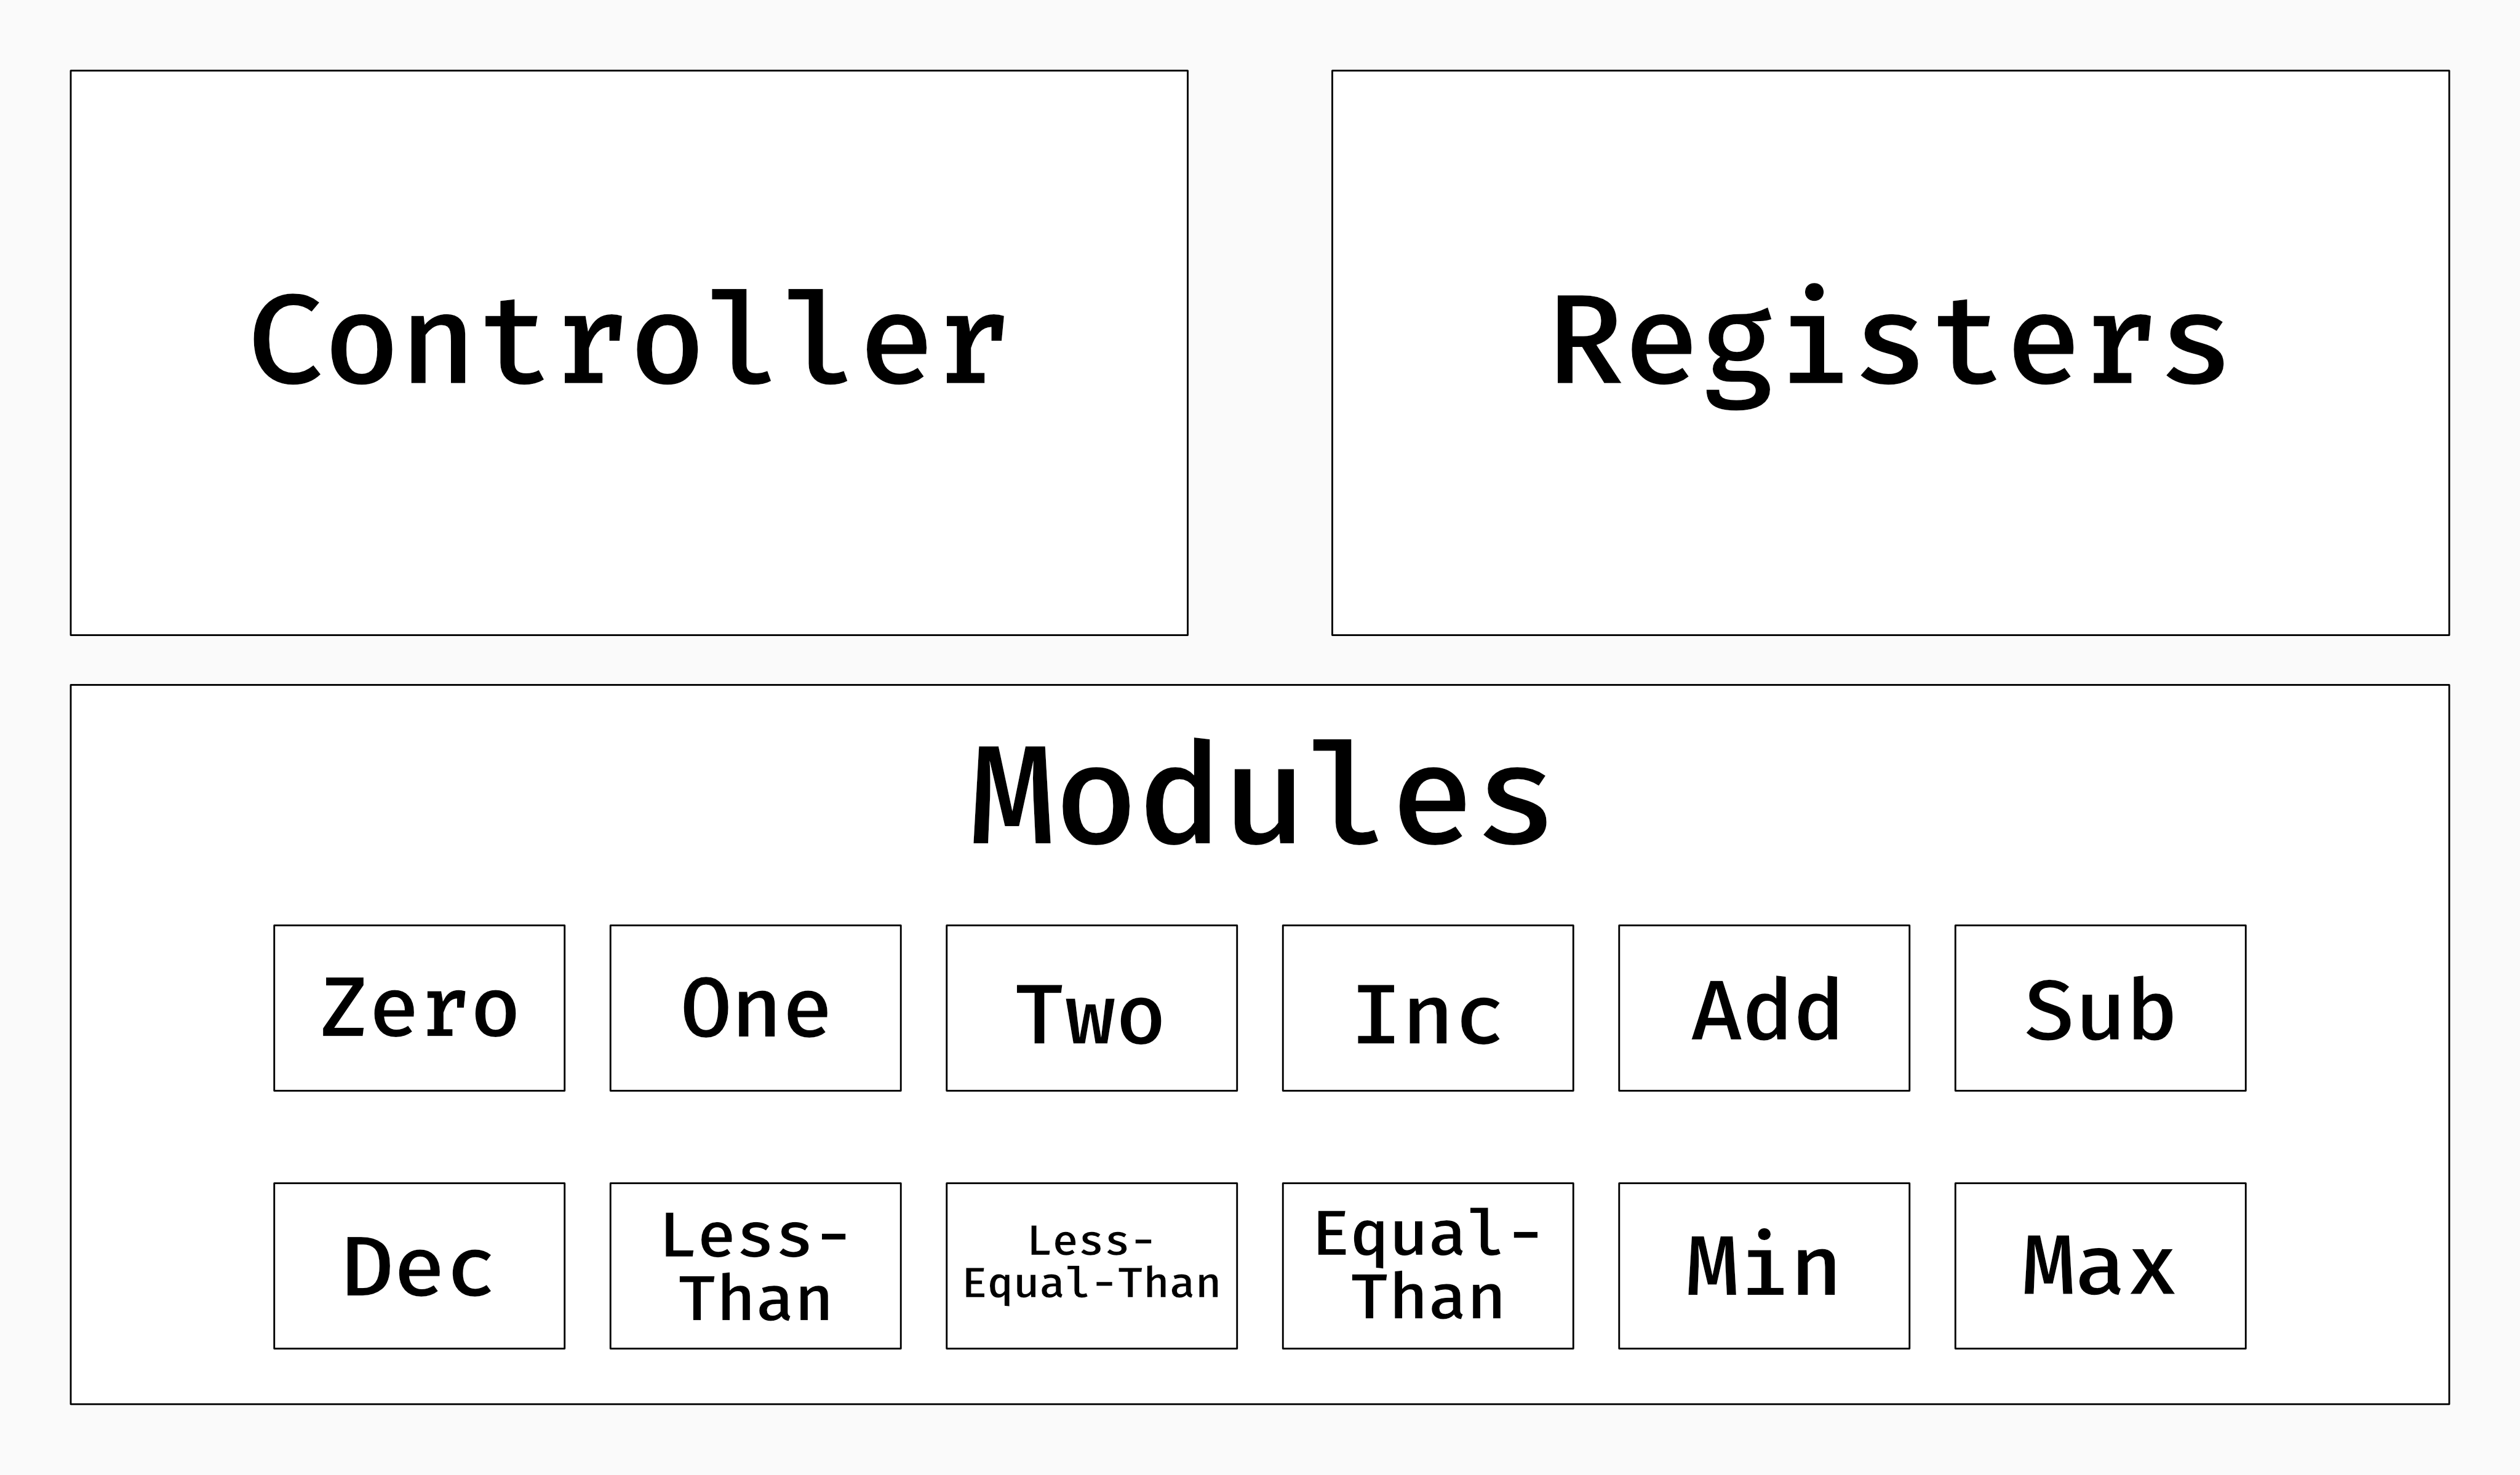
\includegraphics[width=\textwidth]{../figures/schema-nram-without-memory.png}
  	\end{figure}
  \end{frame}
  \begin{frame}{Modules}
  	\begin{figure}
  		\centering
  		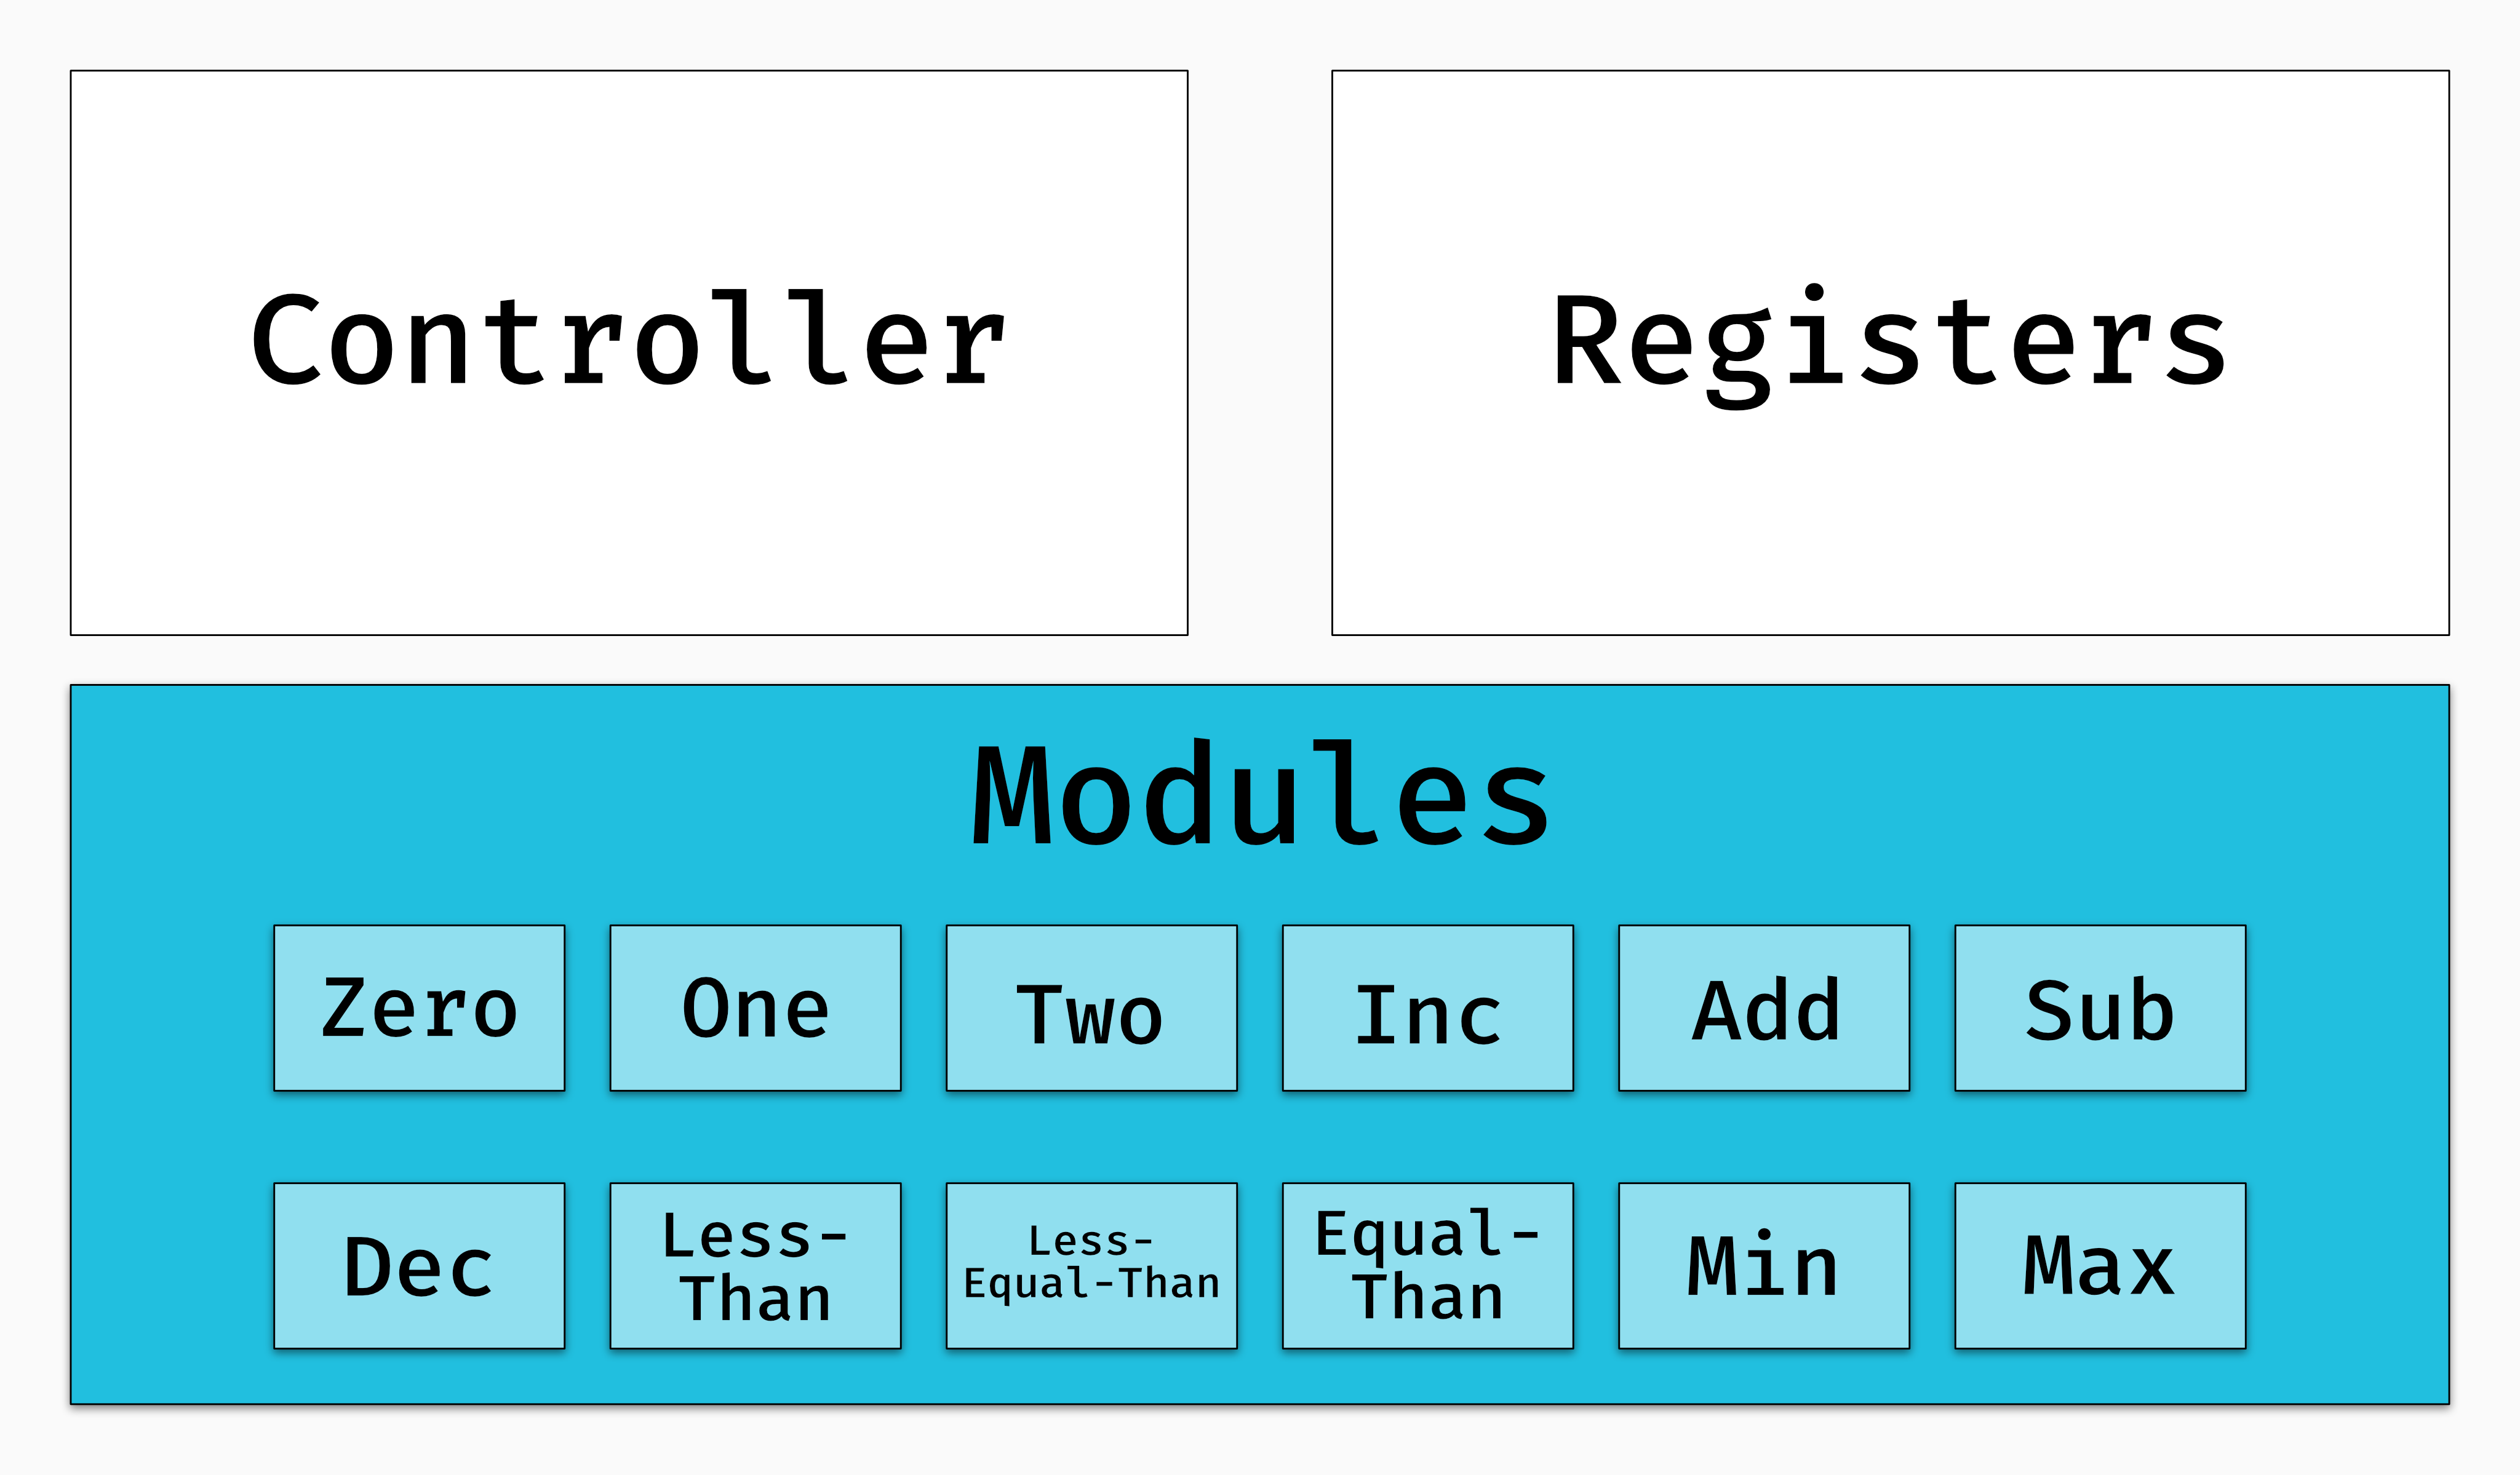
\includegraphics[width=\textwidth]{../figures/schema-nram-without-memory-MS.png}
  	\end{figure}
  \end{frame}
  \begin{frame}{Modules}
  	The modules (or gates) are components through which the controller, connecting them, manipulates values and pointers. In the NRAM exist three types of modules, defined as follows:
  	\begin{align}
		m_i \in N & \textrm{ (Constant modules)} \\
		m_i: p \rightarrow p & \textrm{ (Unary modules)} \\
		m_i: p \times p \rightarrow p & \textrm{ (Binary modules)}
	\end{align}
	Each of them takes as input and returns probability distributions, as exception are constant modules which return only probability distributions.
  \end{frame}
  \begin{frame}{Registers}
  	\begin{figure}
  		\centering
  		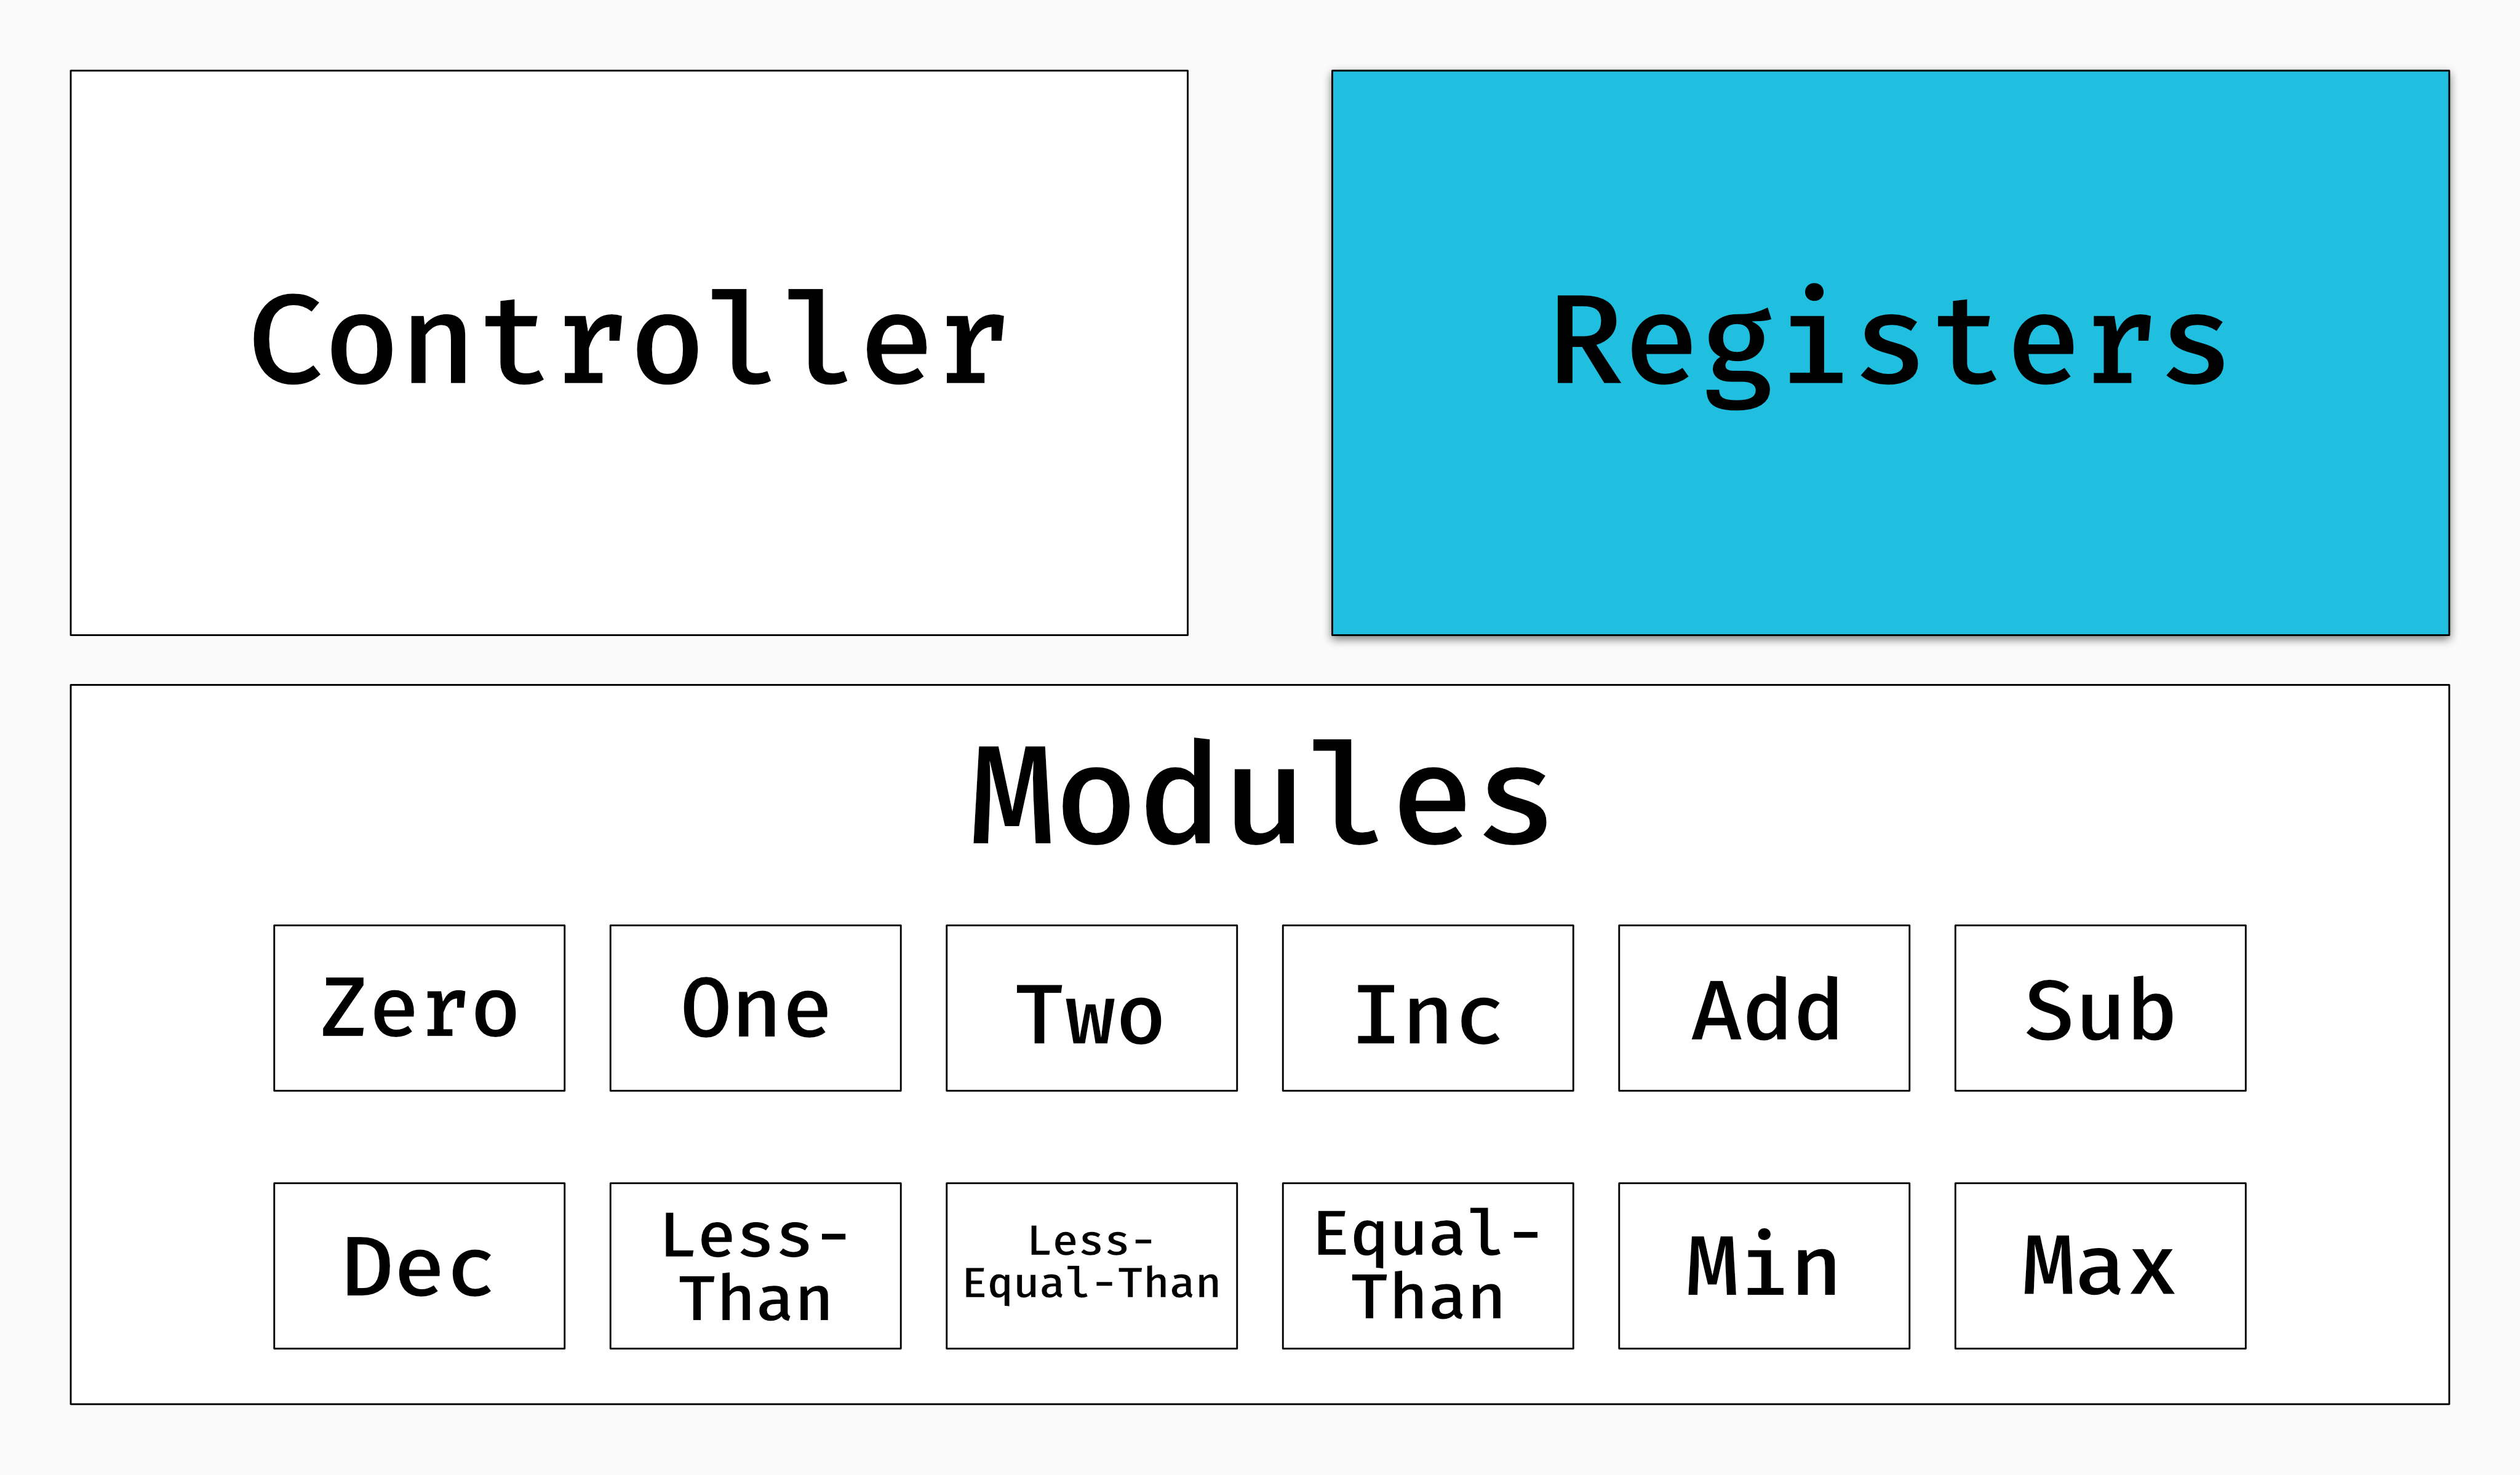
\includegraphics[width=\textwidth]{../figures/schema-nram-without-memory-RS.png}
  	\end{figure}
  \end{frame}
  \begin{frame}{Registers}
  	The registers are a set of memory cells, where each of them contains a probability distribution. Hence, in other words, every register play the role of a random variable.
  \end{frame}
  \begin{frame}{Controller}
  	\begin{figure}
  		\centering
  		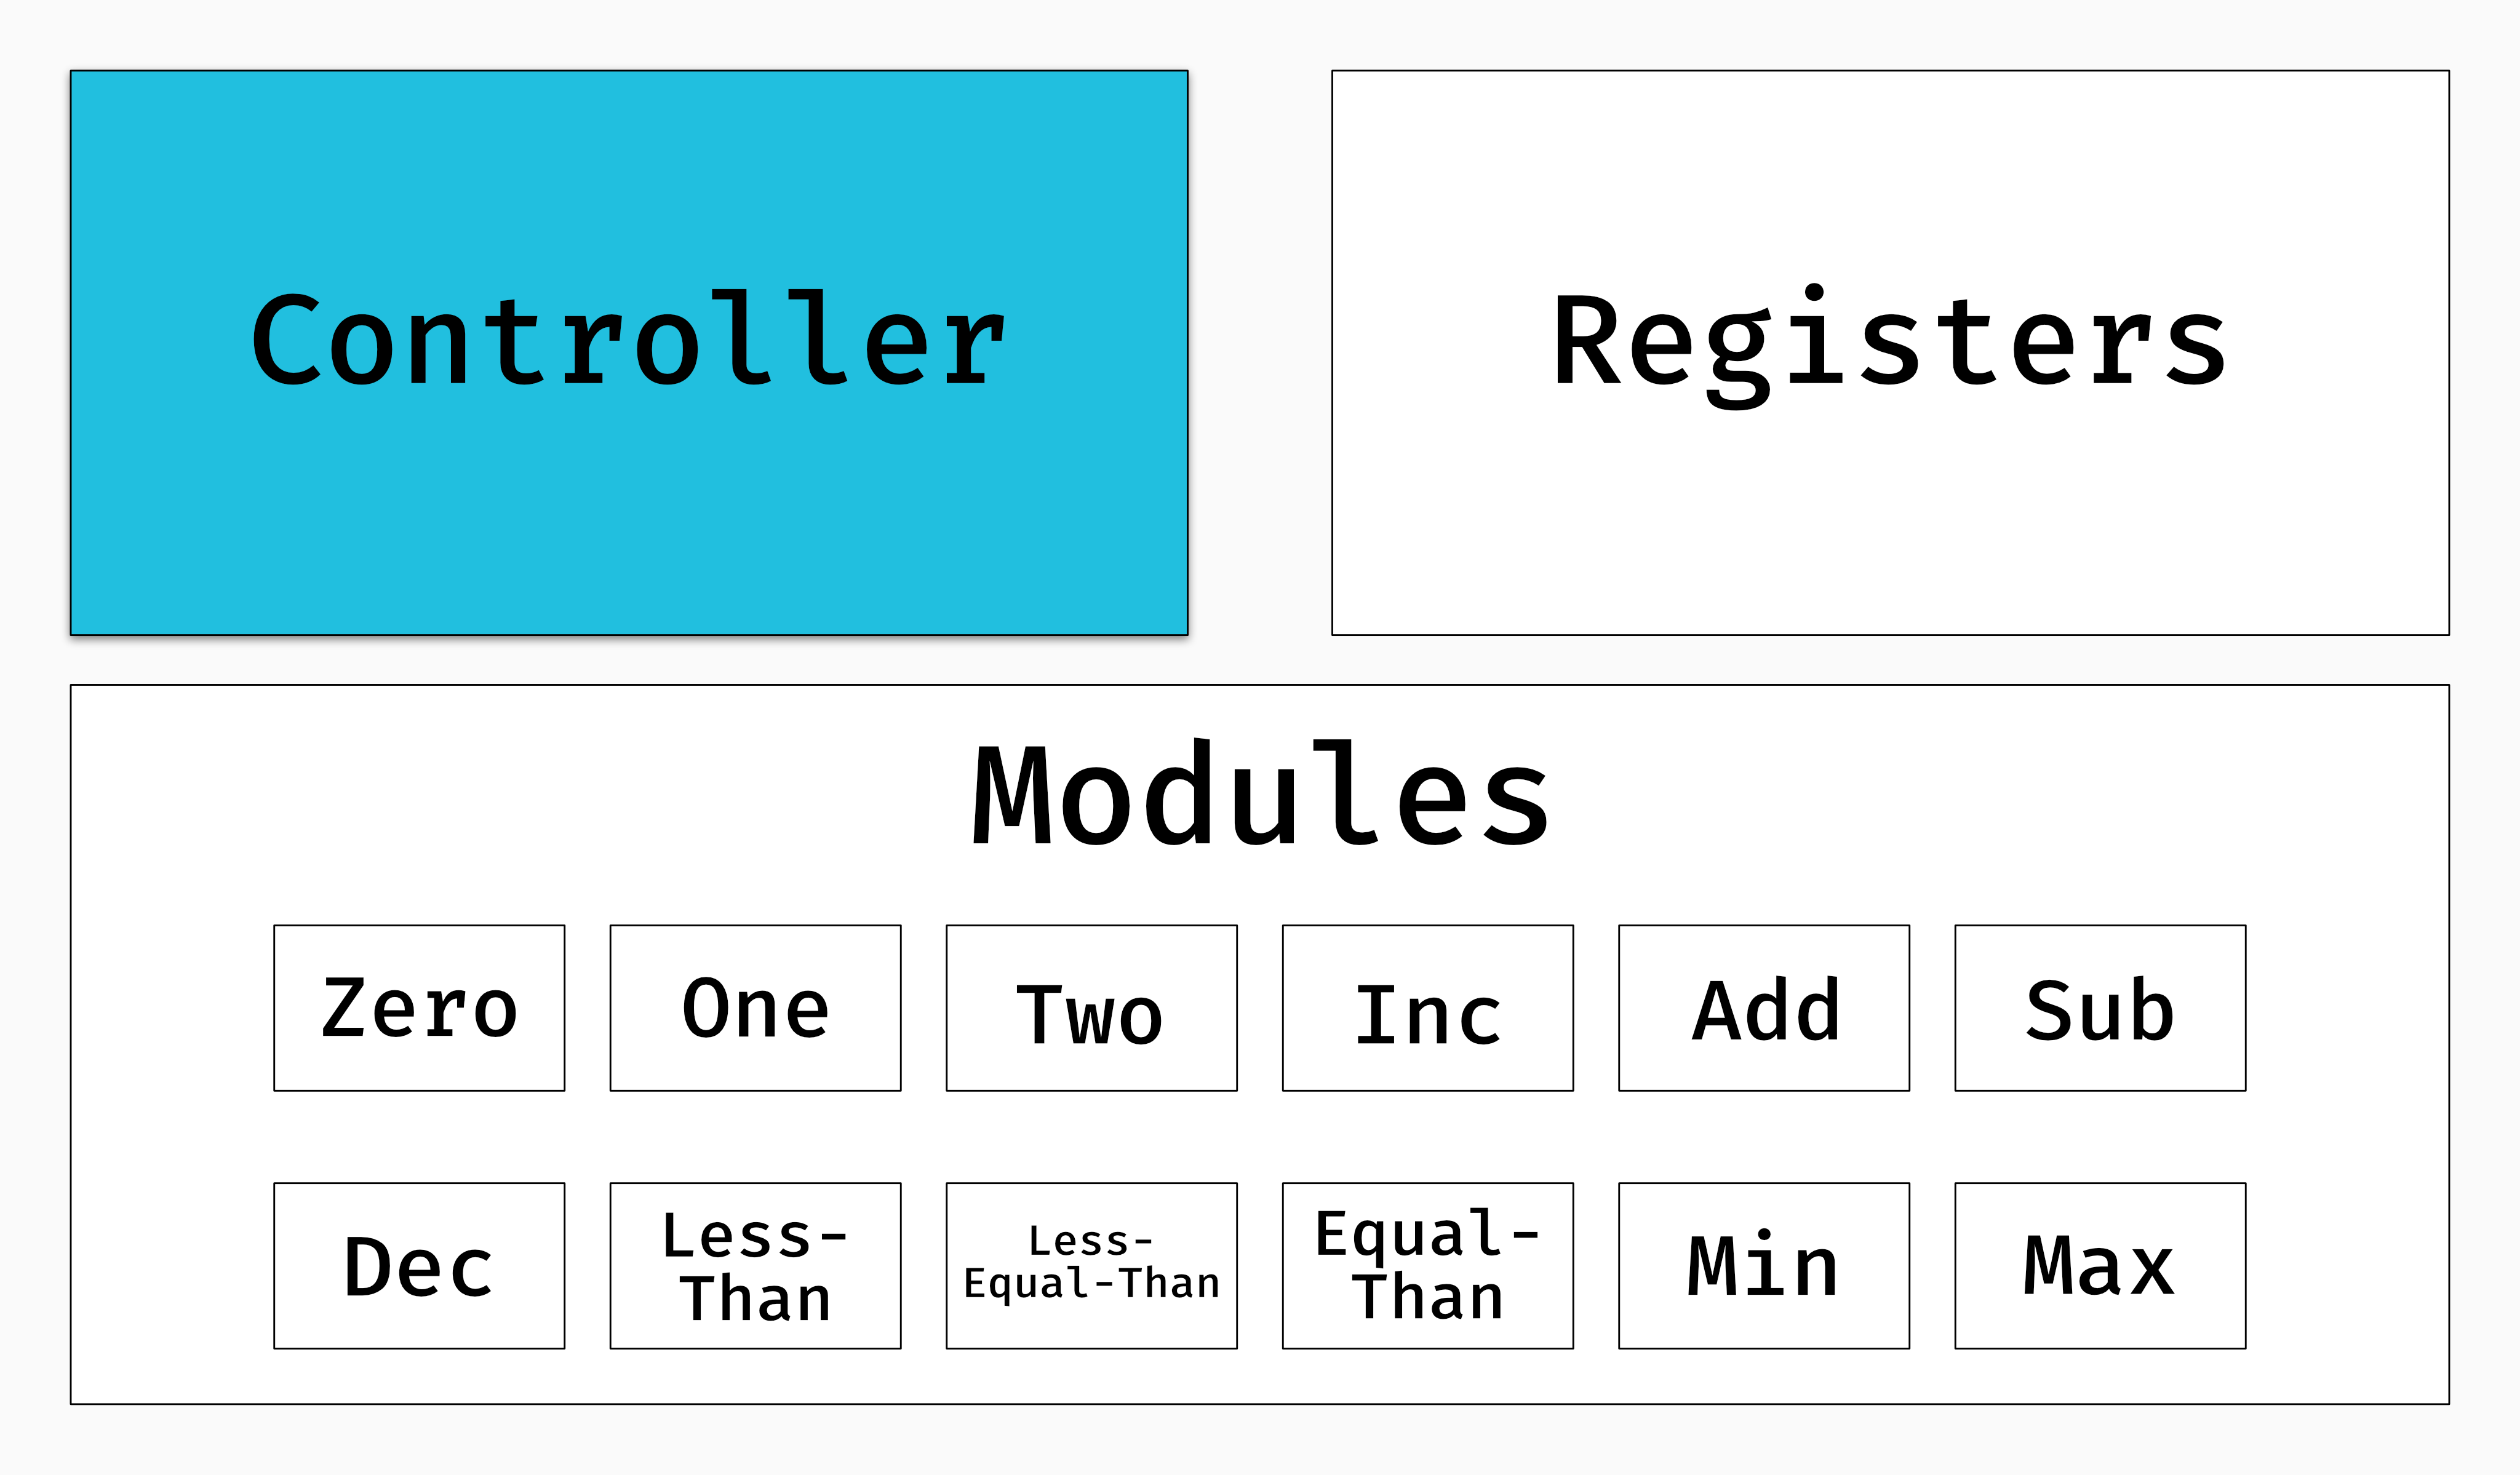
\includegraphics[width=\textwidth]{../figures/schema-nram-without-memory-CL.png}
  	\end{figure}
  \end{frame}
  \begin{frame}{Controller}
  	The controller is a neural network (Multi Layer Perceptron) whose objective is to emit a circuit configuration, i.e. how the circuits are connected together in form of a Directed Acyclic Graph. To do this the controller takes as input the $\mathbb{P}(r_{i} = 0)$ of each register.
  \end{frame}

  \begin{frame}{Timestep execution}  
	\begin{figure}
  		\centering
  		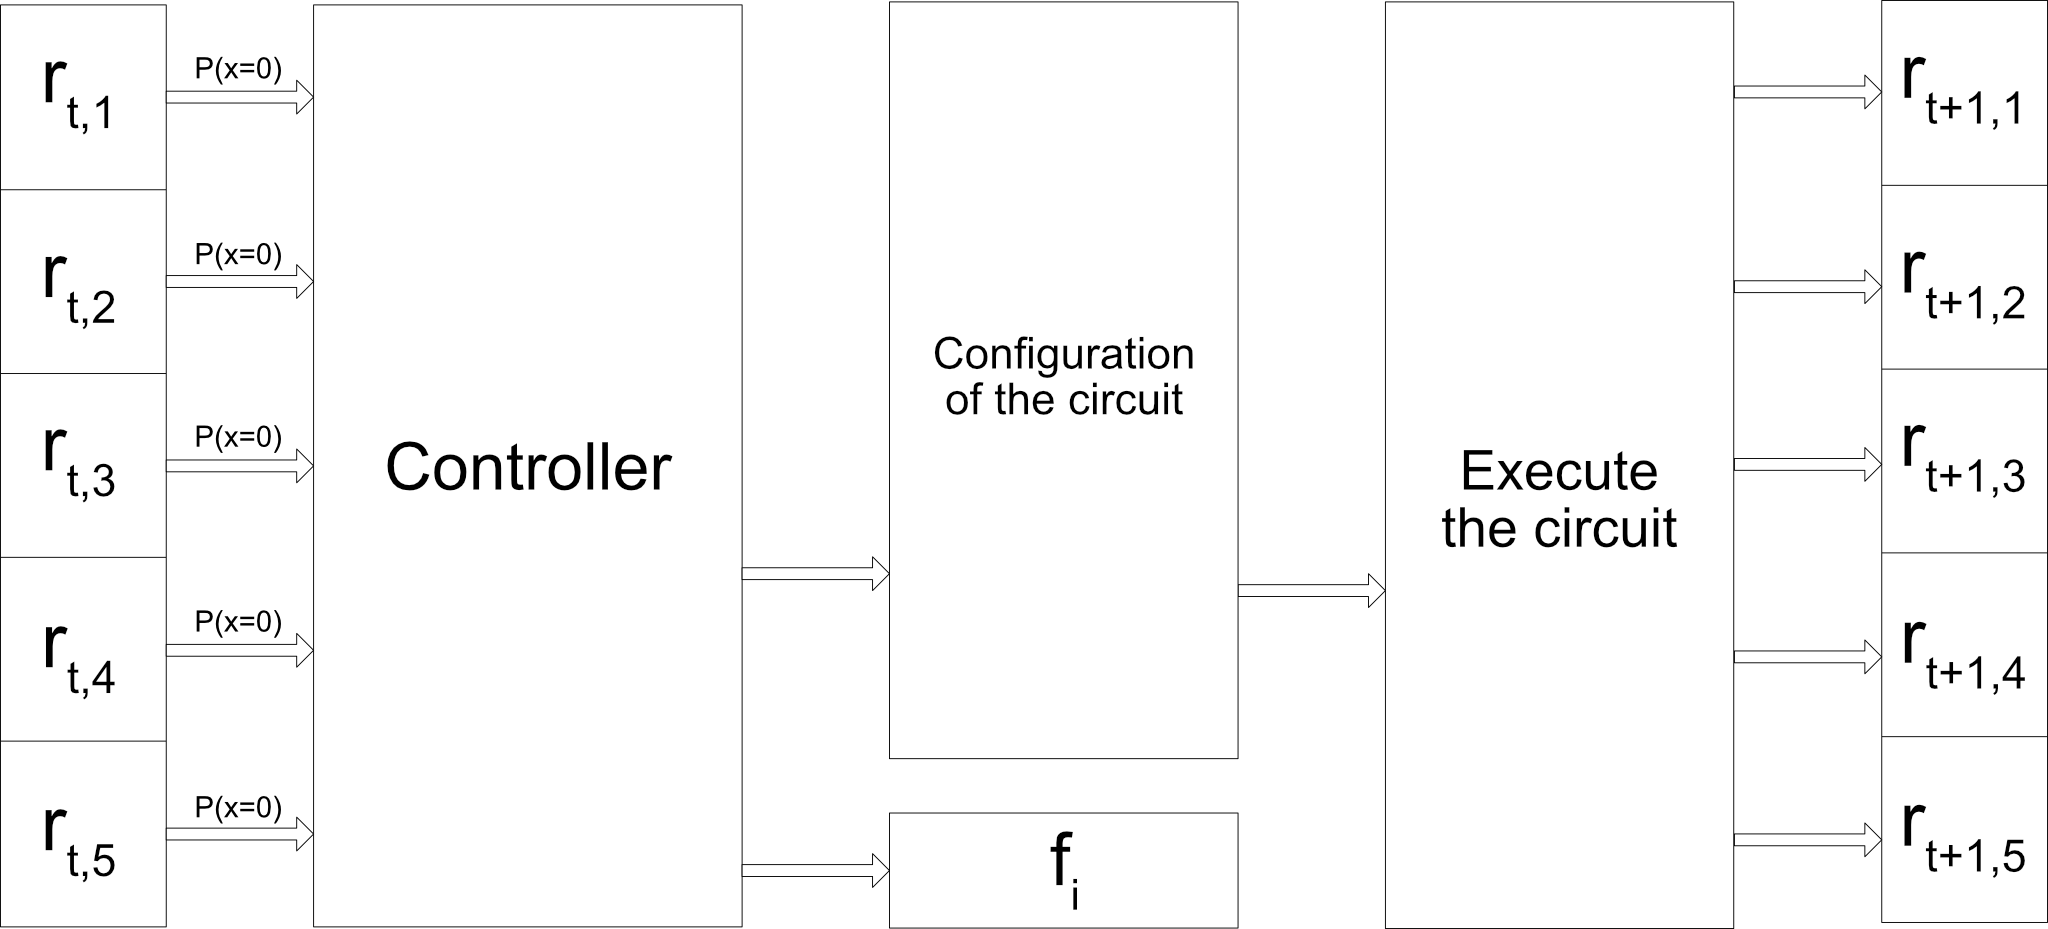
\includegraphics[width=\textwidth]{../figures/timestep-nram-without-memory-execution.png}
  	\end{figure}
  \end{frame}  
  \begin{frame}{Timestep execution - Controller \& Circuit configuration structure}
  	\begin{figure}
  		\centering
  		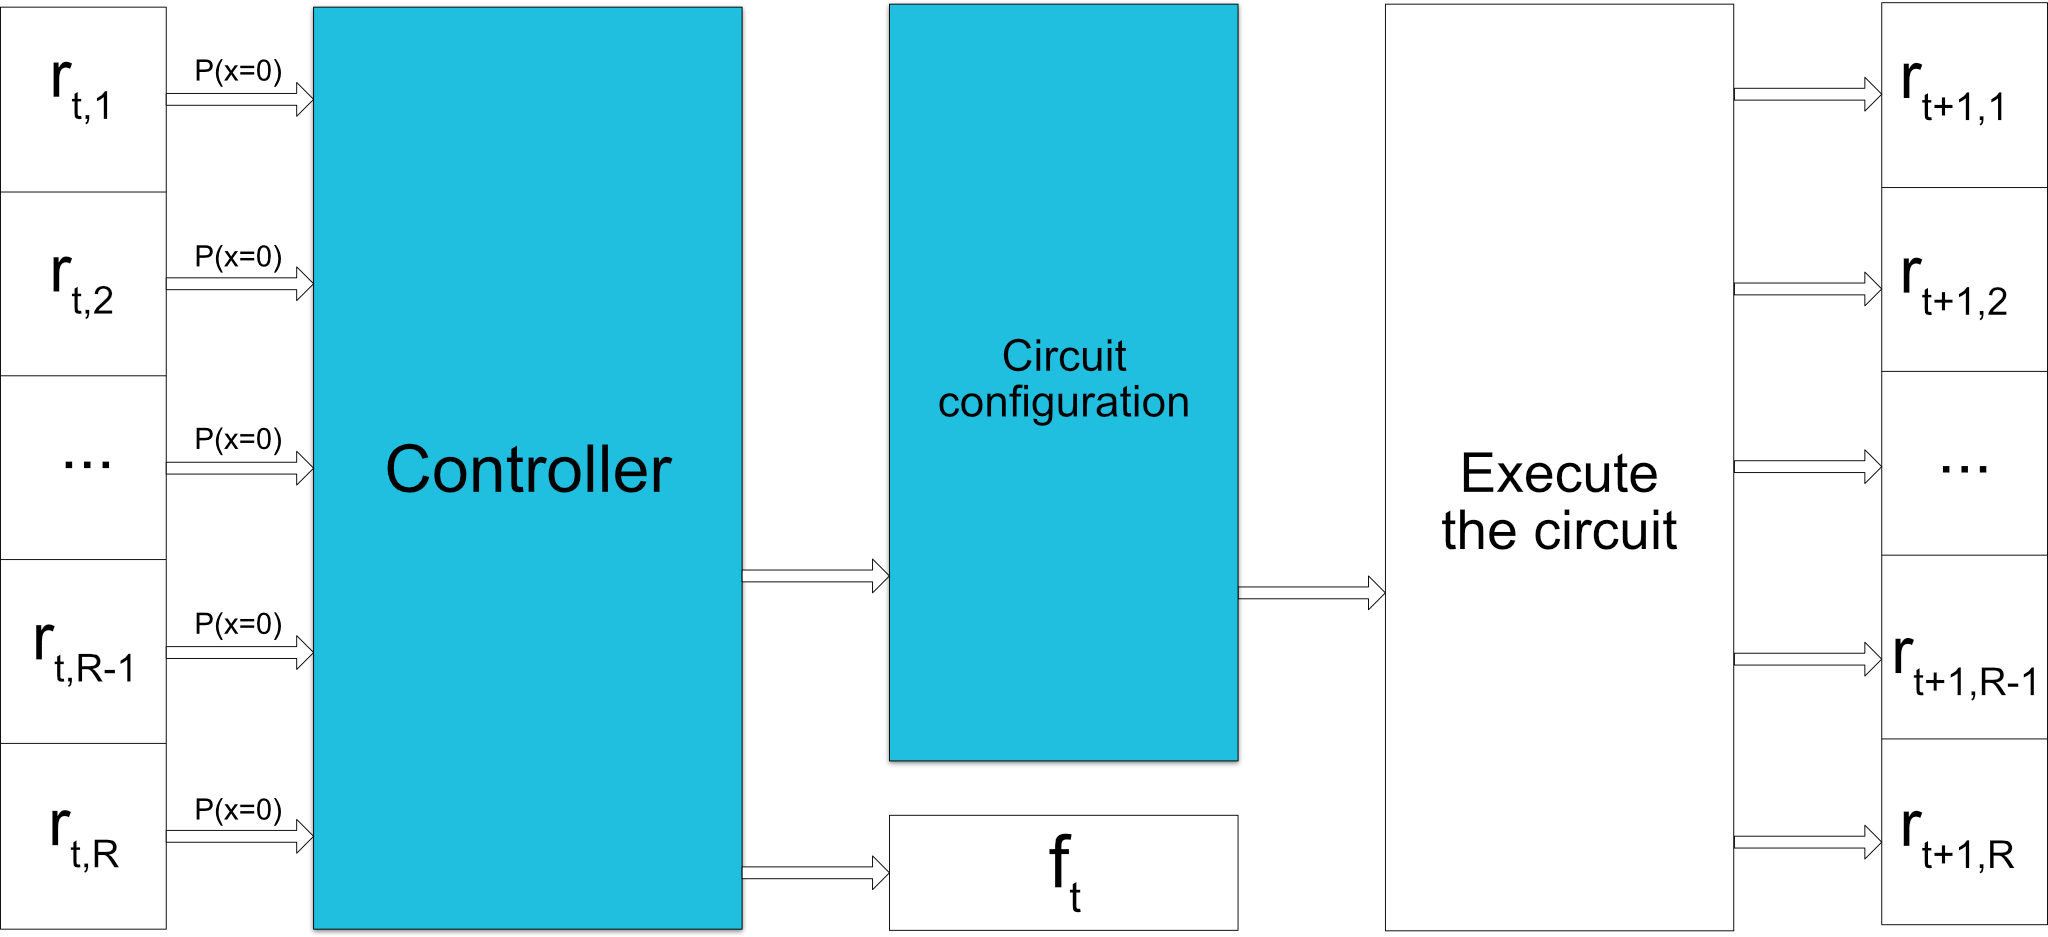
\includegraphics[width=\textwidth]{../figures/timestep-nram-without-memory-execution-CONTROLLER-and-CIRCUIT.png}
  	\end{figure}
  \end{frame}
  \begin{frame}{Timestep execution - Controller}
  	Let $R = 4$ and Gates$ = \{m_u, m_c, m_b\}$, the controller structure appear as follows
  	\begin{figure}
  		\centering
  		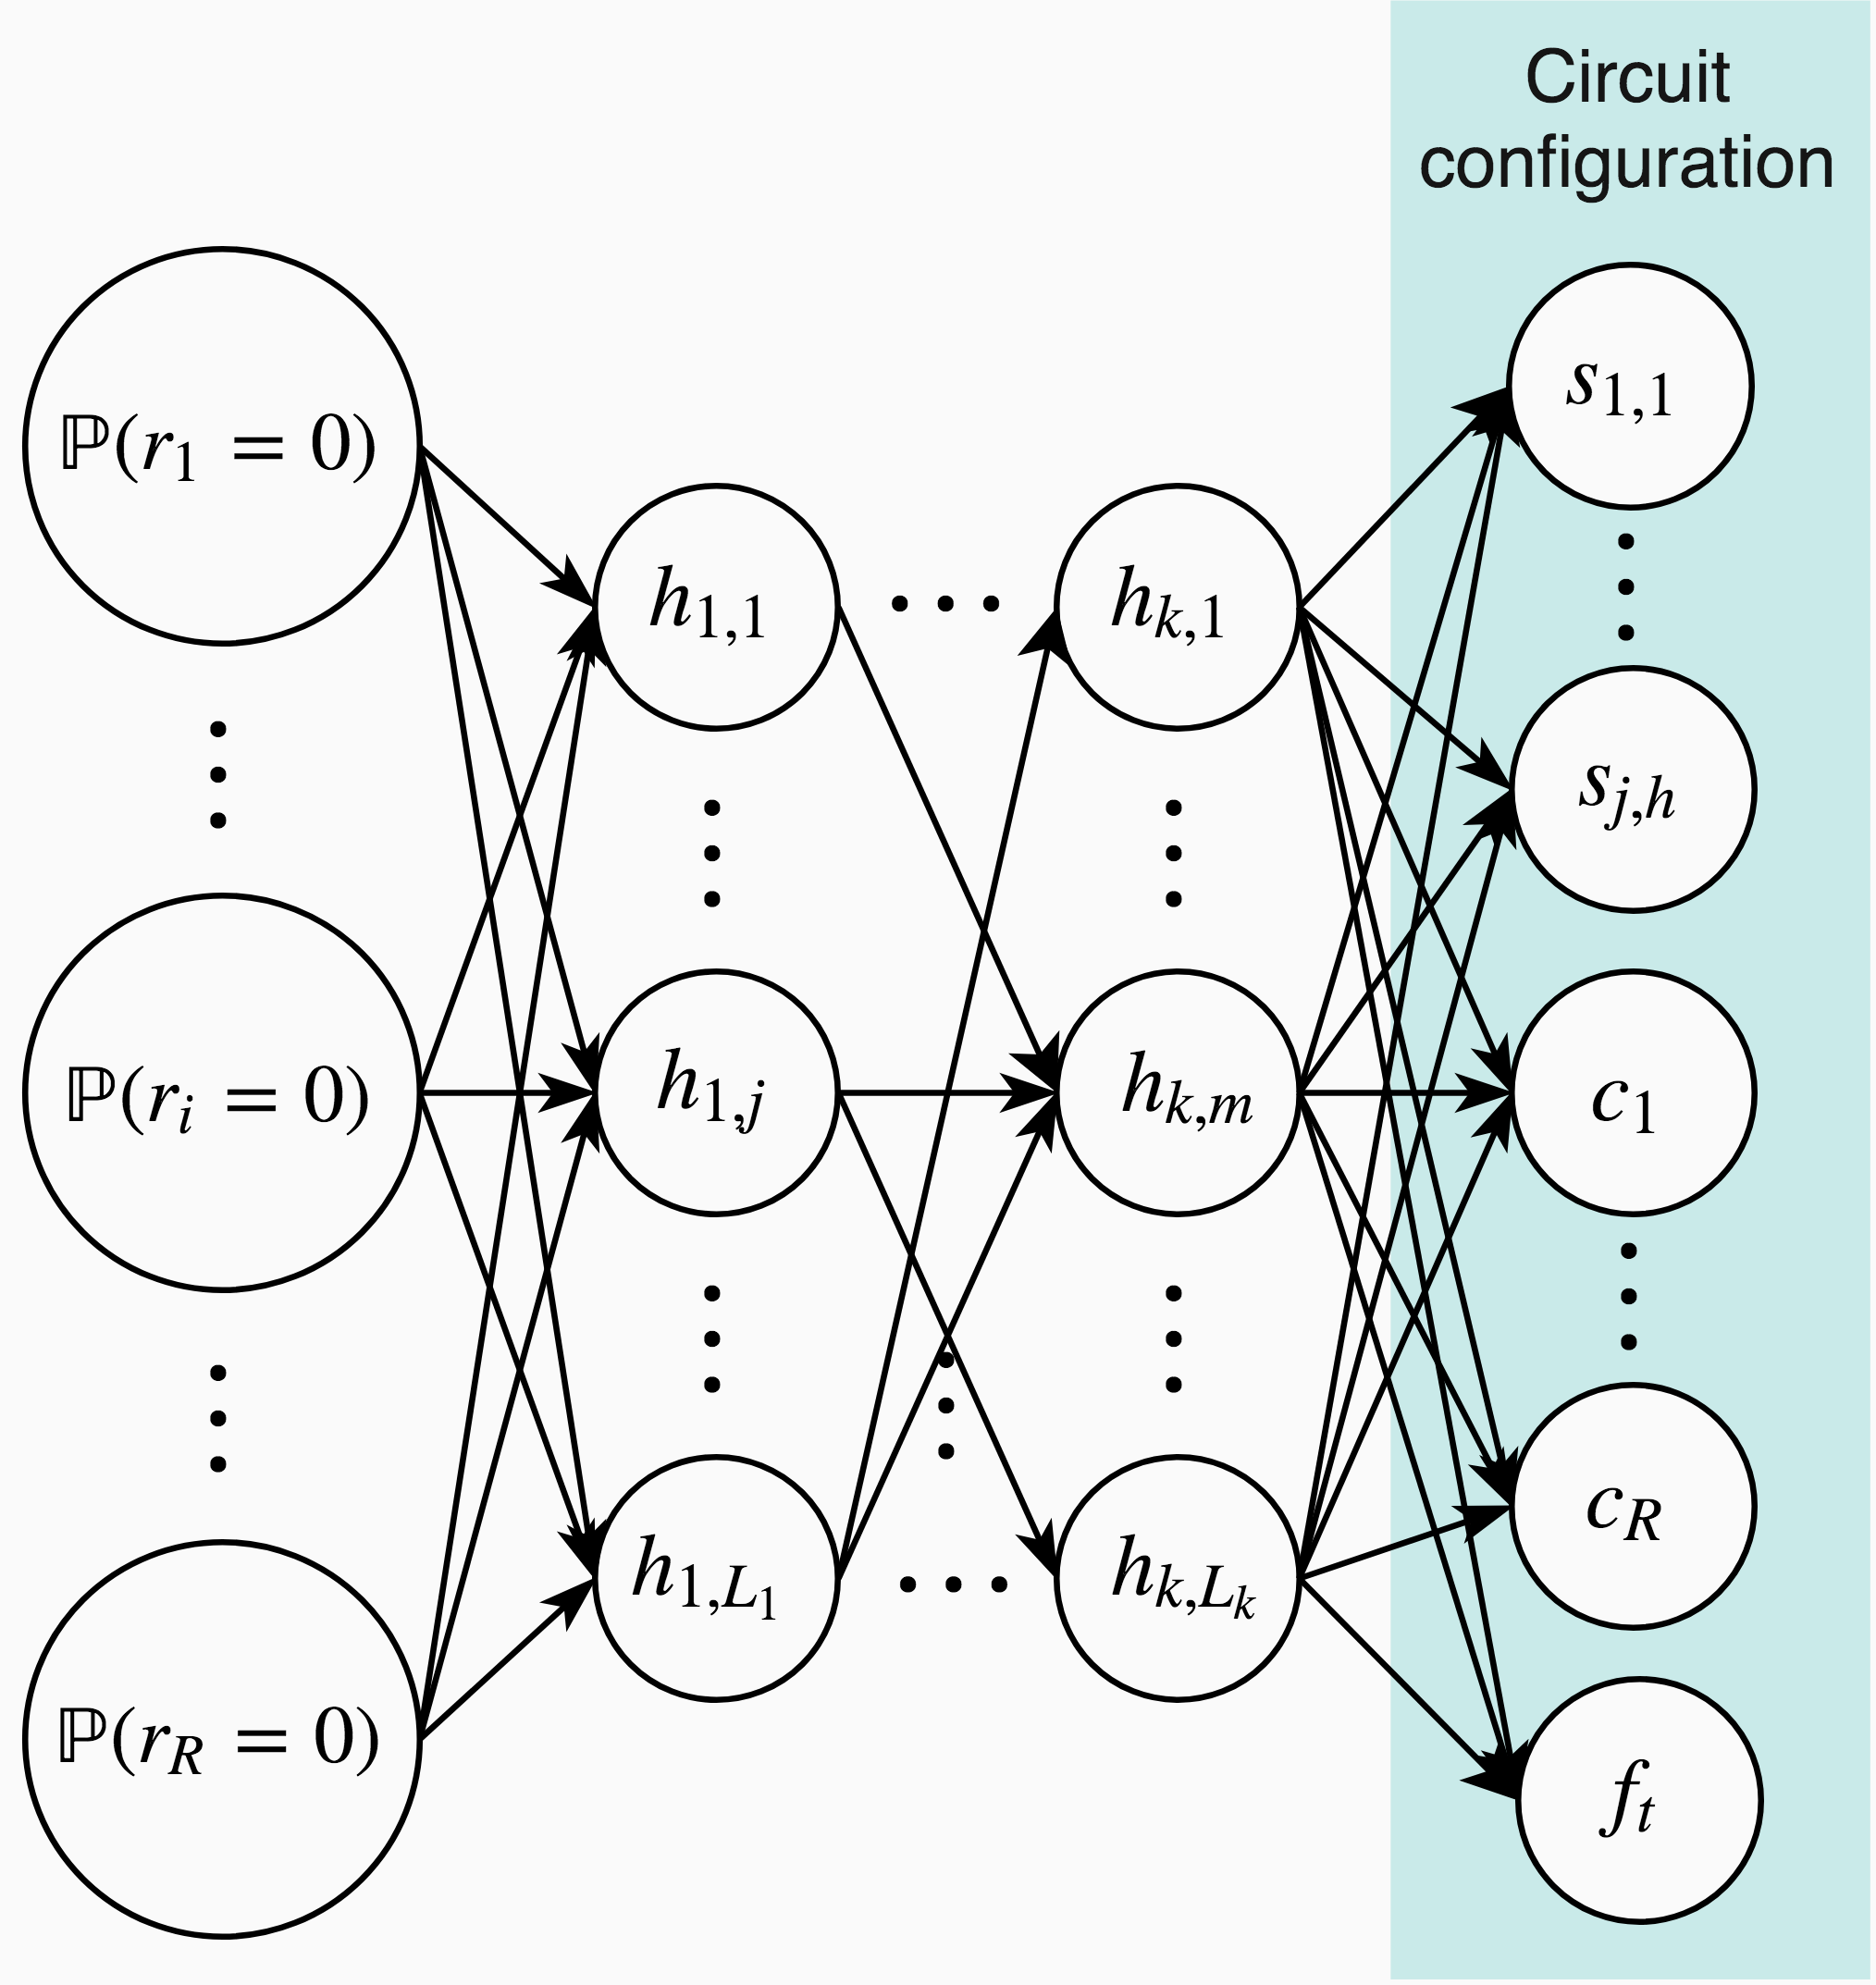
\includegraphics[width=0.65\textwidth]{../figures/nram-mlp.png}
  	\end{figure}
  \end{frame}
  \begin{frame}{Timestep execution - Circuit configuration structure}
  	Using the same assumptions seen in the previous slide, the structure of the circuit configuration is represented as a list of vectors as follows
  	\begin{table}
  		\centering
  		\begin{tabular}{|c|c|c|c|c|c|c|c|}
  			\hline
  			\cellcolor{mLightGray} $softmax(a_u)$ & 0 & 0 & 0 & 1 & \multicolumn{3}{c|}{} \\ \hline
  			\cellcolor{mLightGray} $softmax(a_{b})$ & 0 & 0 & 0.4 & 0 & 0.7 & 0 &  \\ \hline
  			\cellcolor{mLightGray} $softmax(b_{b})$ & 0 & 0.4 & 0.1 & 0.1 & 0.3 & 0.1 &  \\ \hline
  			\cellcolor{mLightGray} $softmax(c_{0})$ & 0.2 & 0.2 & 0.3 & 0.1 & 0.2 & 0 & 0\\ \hline
  			\cellcolor{mLightGray} $softmax(c_{1})$ & 0.3 & 0.1 & 0.1 & 0.4 & 0 & 0.1 & 0 \\ \hline
  			\cellcolor{mLightGray} $softmax(c_{2})$ & 0.6 & 0.3 & 0.1 & 0 & 0 & 0 & 0 \\ \hline
  			\cellcolor{mLightGray} $softmax(c_{3})$ & 0 & 1 & 0 & 0 & 0 & 0 & 0 \\ \hline
  			\cellcolor{mLightGray} $\sigma(f_{t})$ & 0.3 & \multicolumn{6}{c|}{} \\ \hline
  		\end{tabular}
  	\end{table}
  \end{frame}
  
  \begin{frame}{Timestep execution - Selection of the input of the gates}
  	 An input for the gate $m_i$ is chosen by the controller from the set $\{r_{1}, \dots, r_{R}, o_{1}, \dots, o_{i-1}\}$ where:
	\begin{itemize}
		\item $r_j$ is the content of the $j^{th}$ register, $j=1,\dots,R$;
	\item $o_k$ is the output of the $k^{th}$ previous gate with respect to the current $m_i$, for $k=1,\dots,|Gates| - 1$.
	\end{itemize}
selected through a weighted average with a coefficient $s_{i}$ as follows
	\begin{center}
		$(r_1, r_2, \dots, r_R, o_1, o_2, \dots, o_{i-1})^T\textbf{softmax}(s_i)$
	\end{center}
  \end{frame}
  \begin{frame}{Timestep execution - Selection of the input of the registers}
  	Similarly to the gates, also the content of the registers is updated as follows:
	\begin{center}
		$r_i^{(t + 1)} = (r_1^{(t)}, \dots, r_R^{(t)}, o_1^{(t)}, \dots, o_{|\textrm{Gates}|}^{(t)})^T\textbf{softmax}(s_i)$
	\end{center}
  \end{frame}  
  
  \begin{frame}{Timestep execution - Circuit execution example}
  	\begin{figure}
  		\centering
  		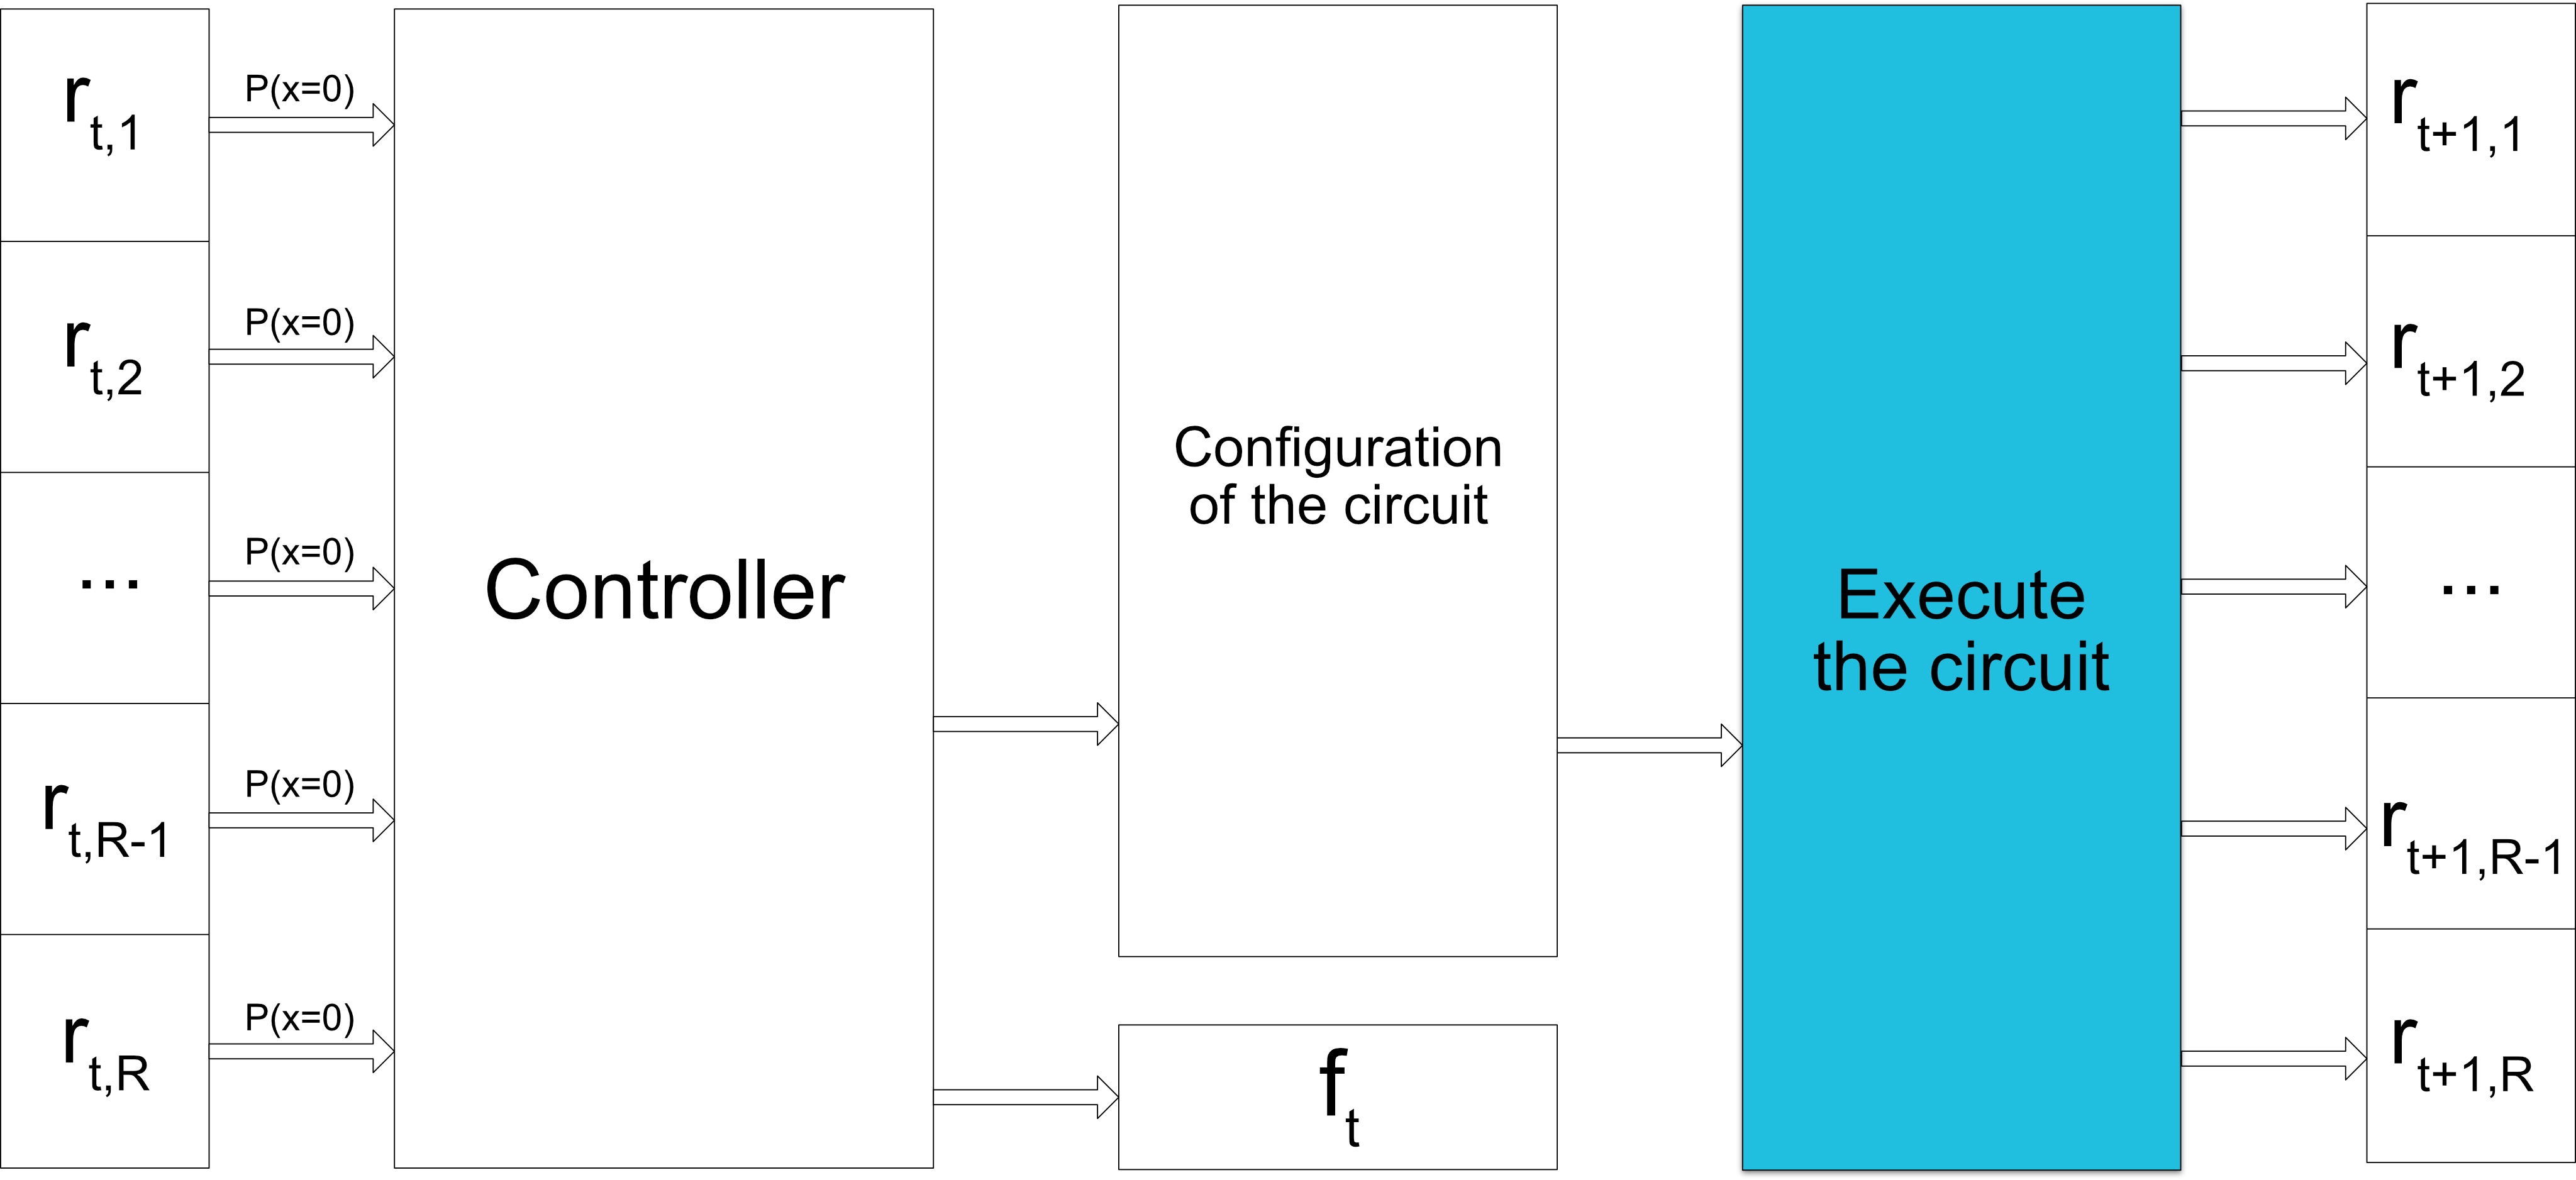
\includegraphics[width=\textwidth]{../figures/timestep-nram-without-memory-execution-CIRCUIT.png}
  	\end{figure}
  \end{frame}
  \begin{frame}{Timestep execution - Circuit execution example}
  	\begin{figure}
  		\centering
  		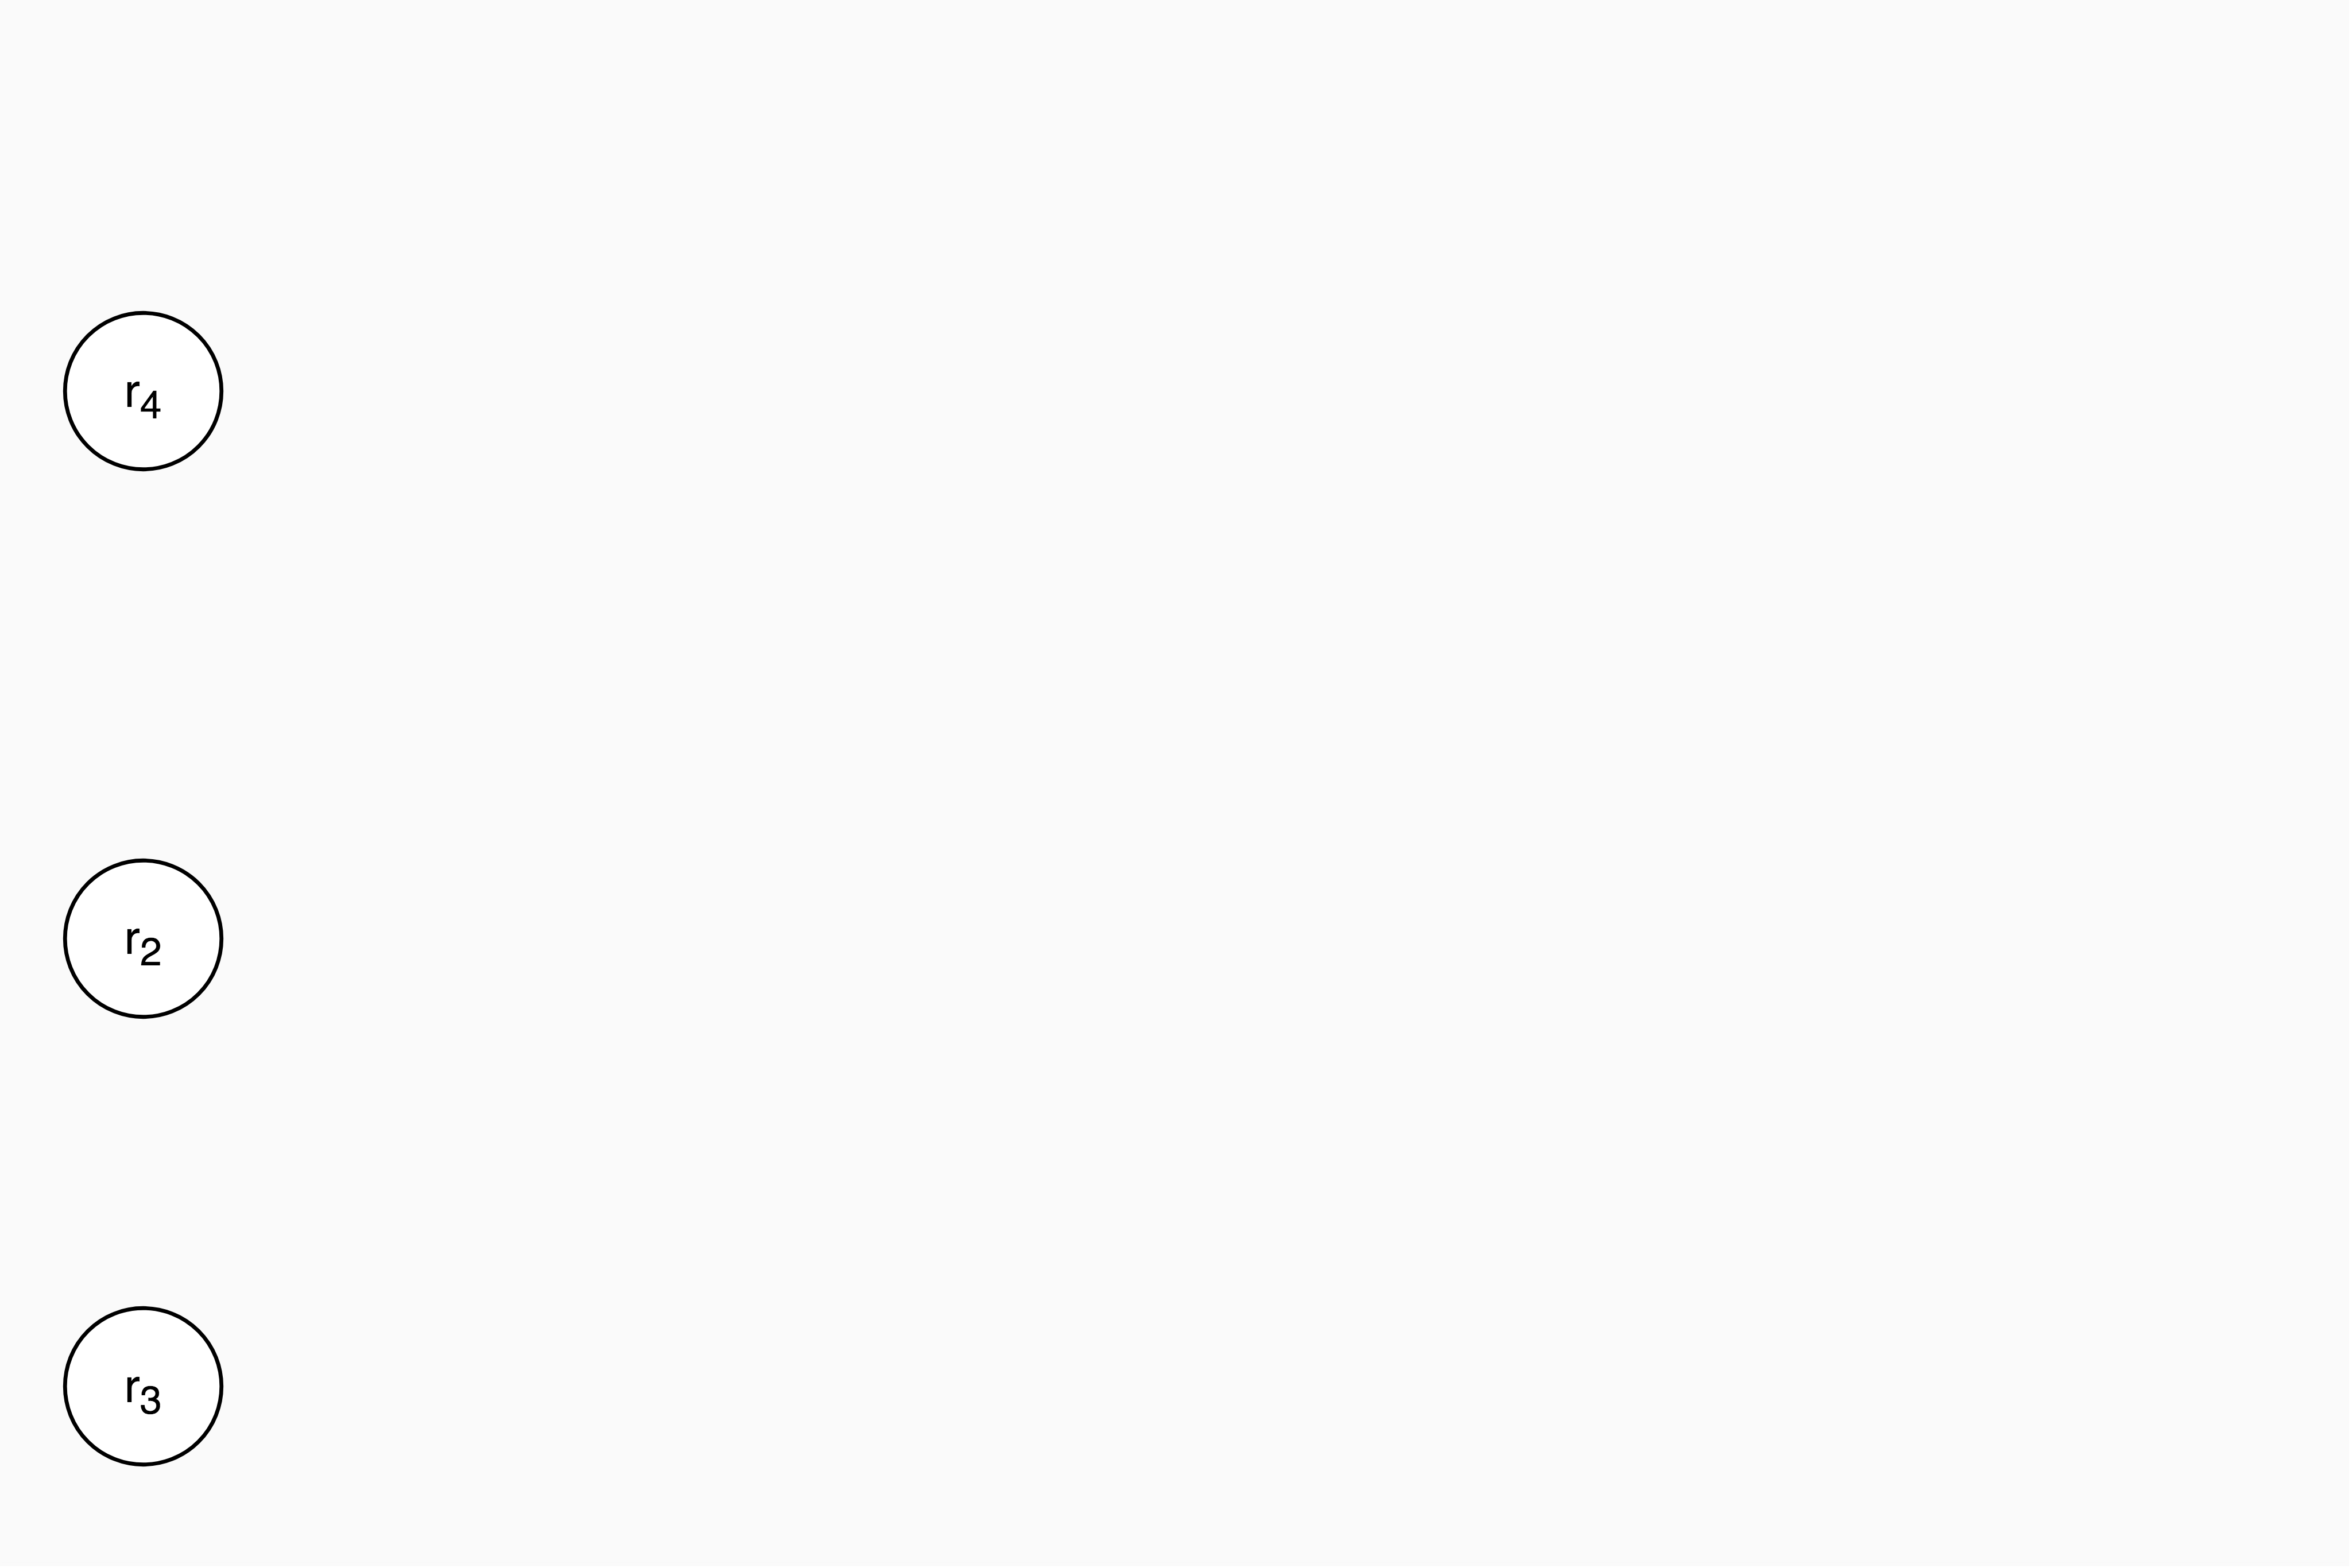
\includegraphics[width=\textwidth]{../figures/example-circuit-0.png}
  	\end{figure}
  \end{frame}
  \begin{frame}{Timestep execution - Circuit execution example}
  	\begin{figure}
  		\centering
  		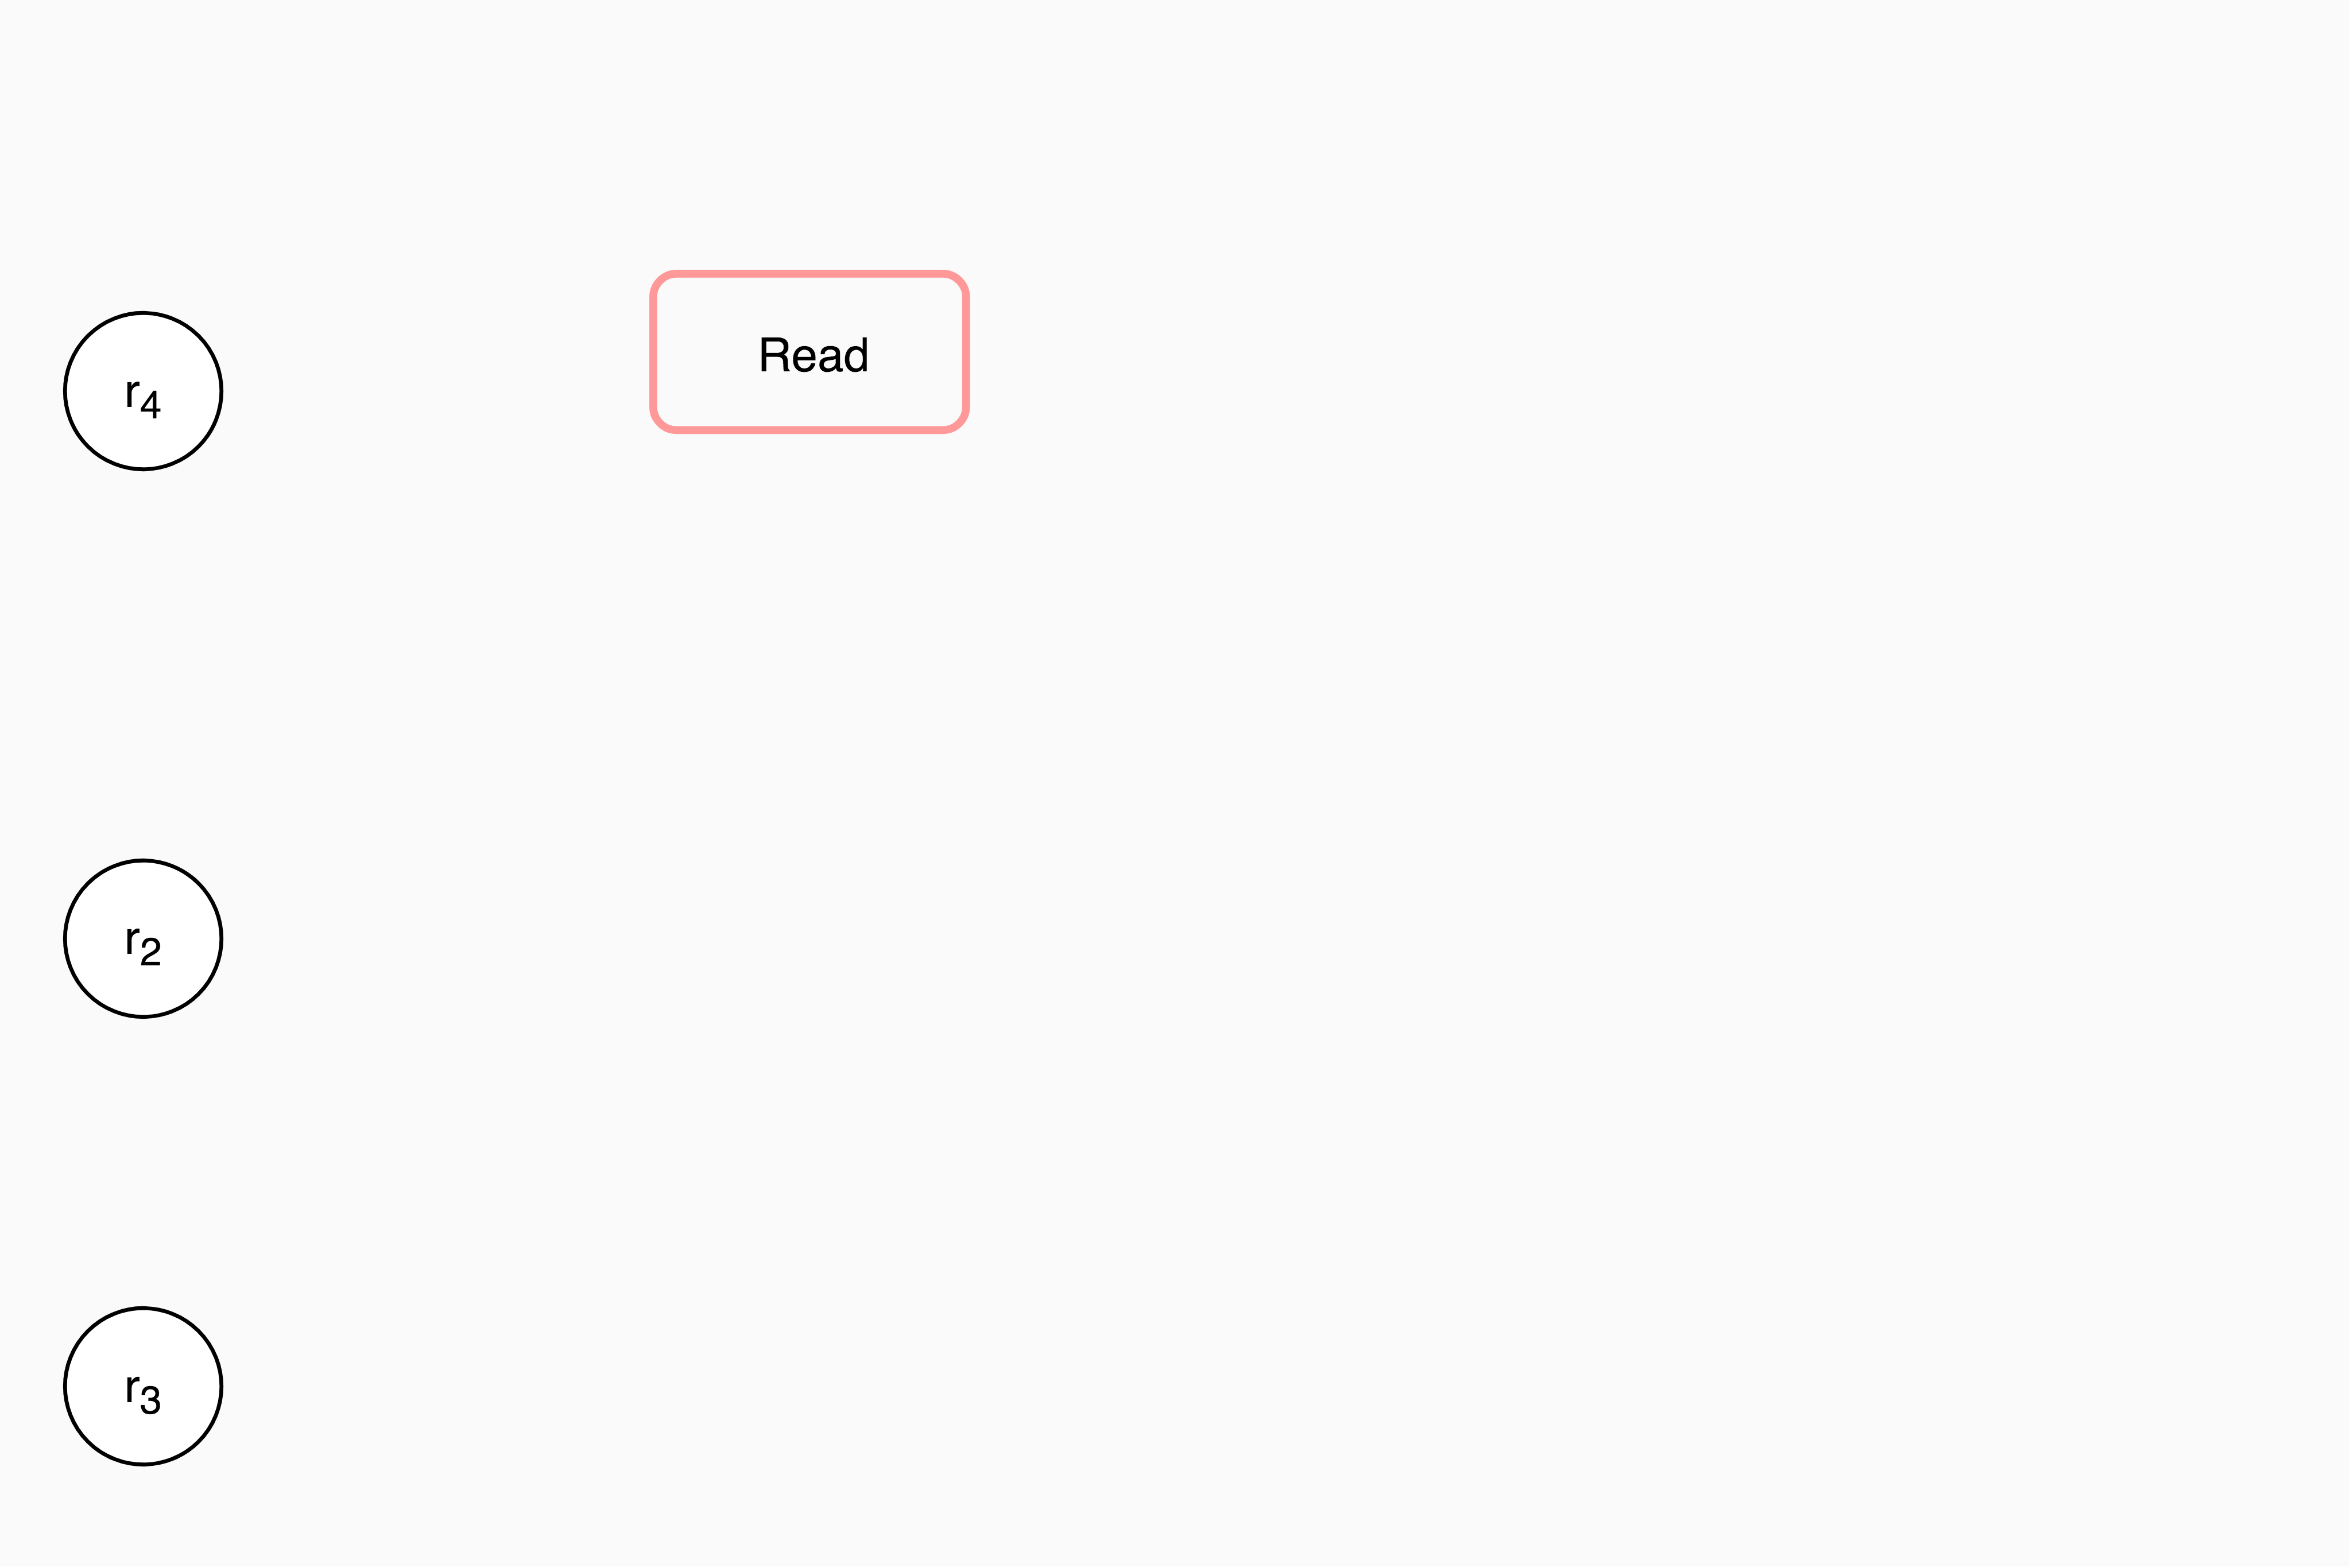
\includegraphics[width=\textwidth]{../figures/example-circuit-1.png}
  	\end{figure}
  \end{frame}
  \begin{frame}{Timestep execution - Circuit execution example}
  	\begin{figure}
  		\centering
  		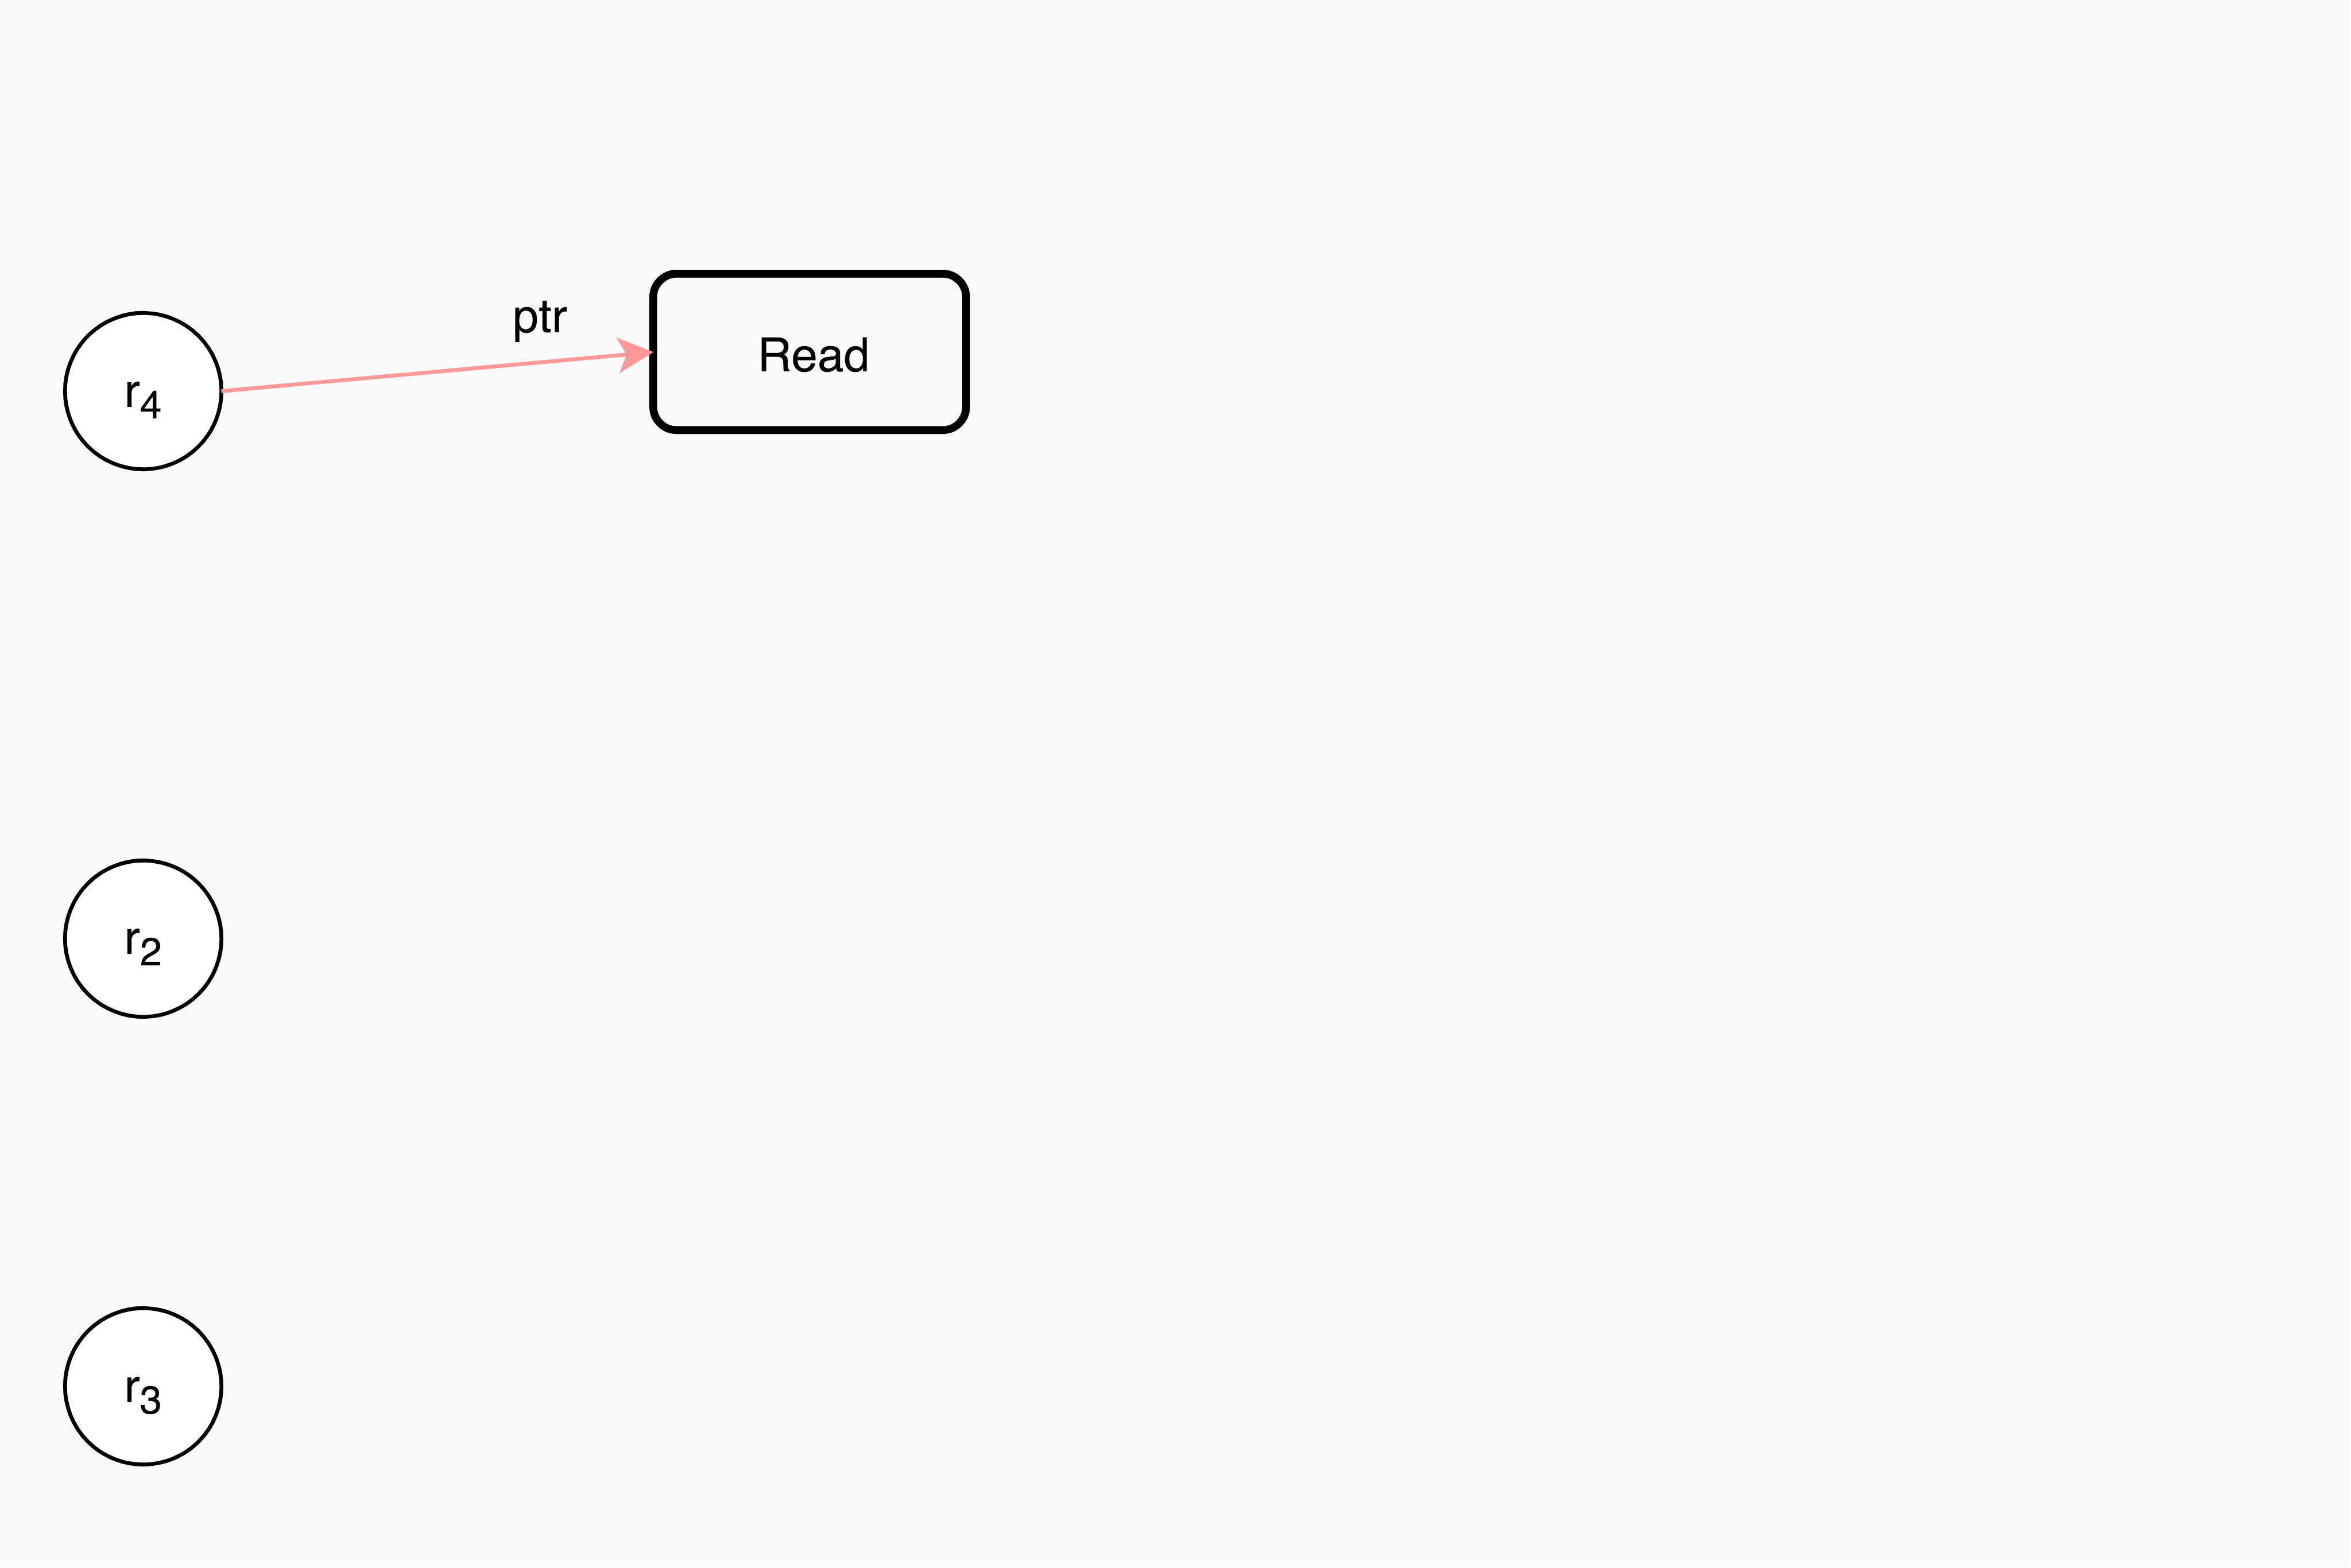
\includegraphics[width=\textwidth]{../figures/example-circuit-2.png}
  	\end{figure}
  \end{frame}
  \begin{frame}{Timestep execution - Circuit execution example}
  	\begin{figure}
  		\centering
  		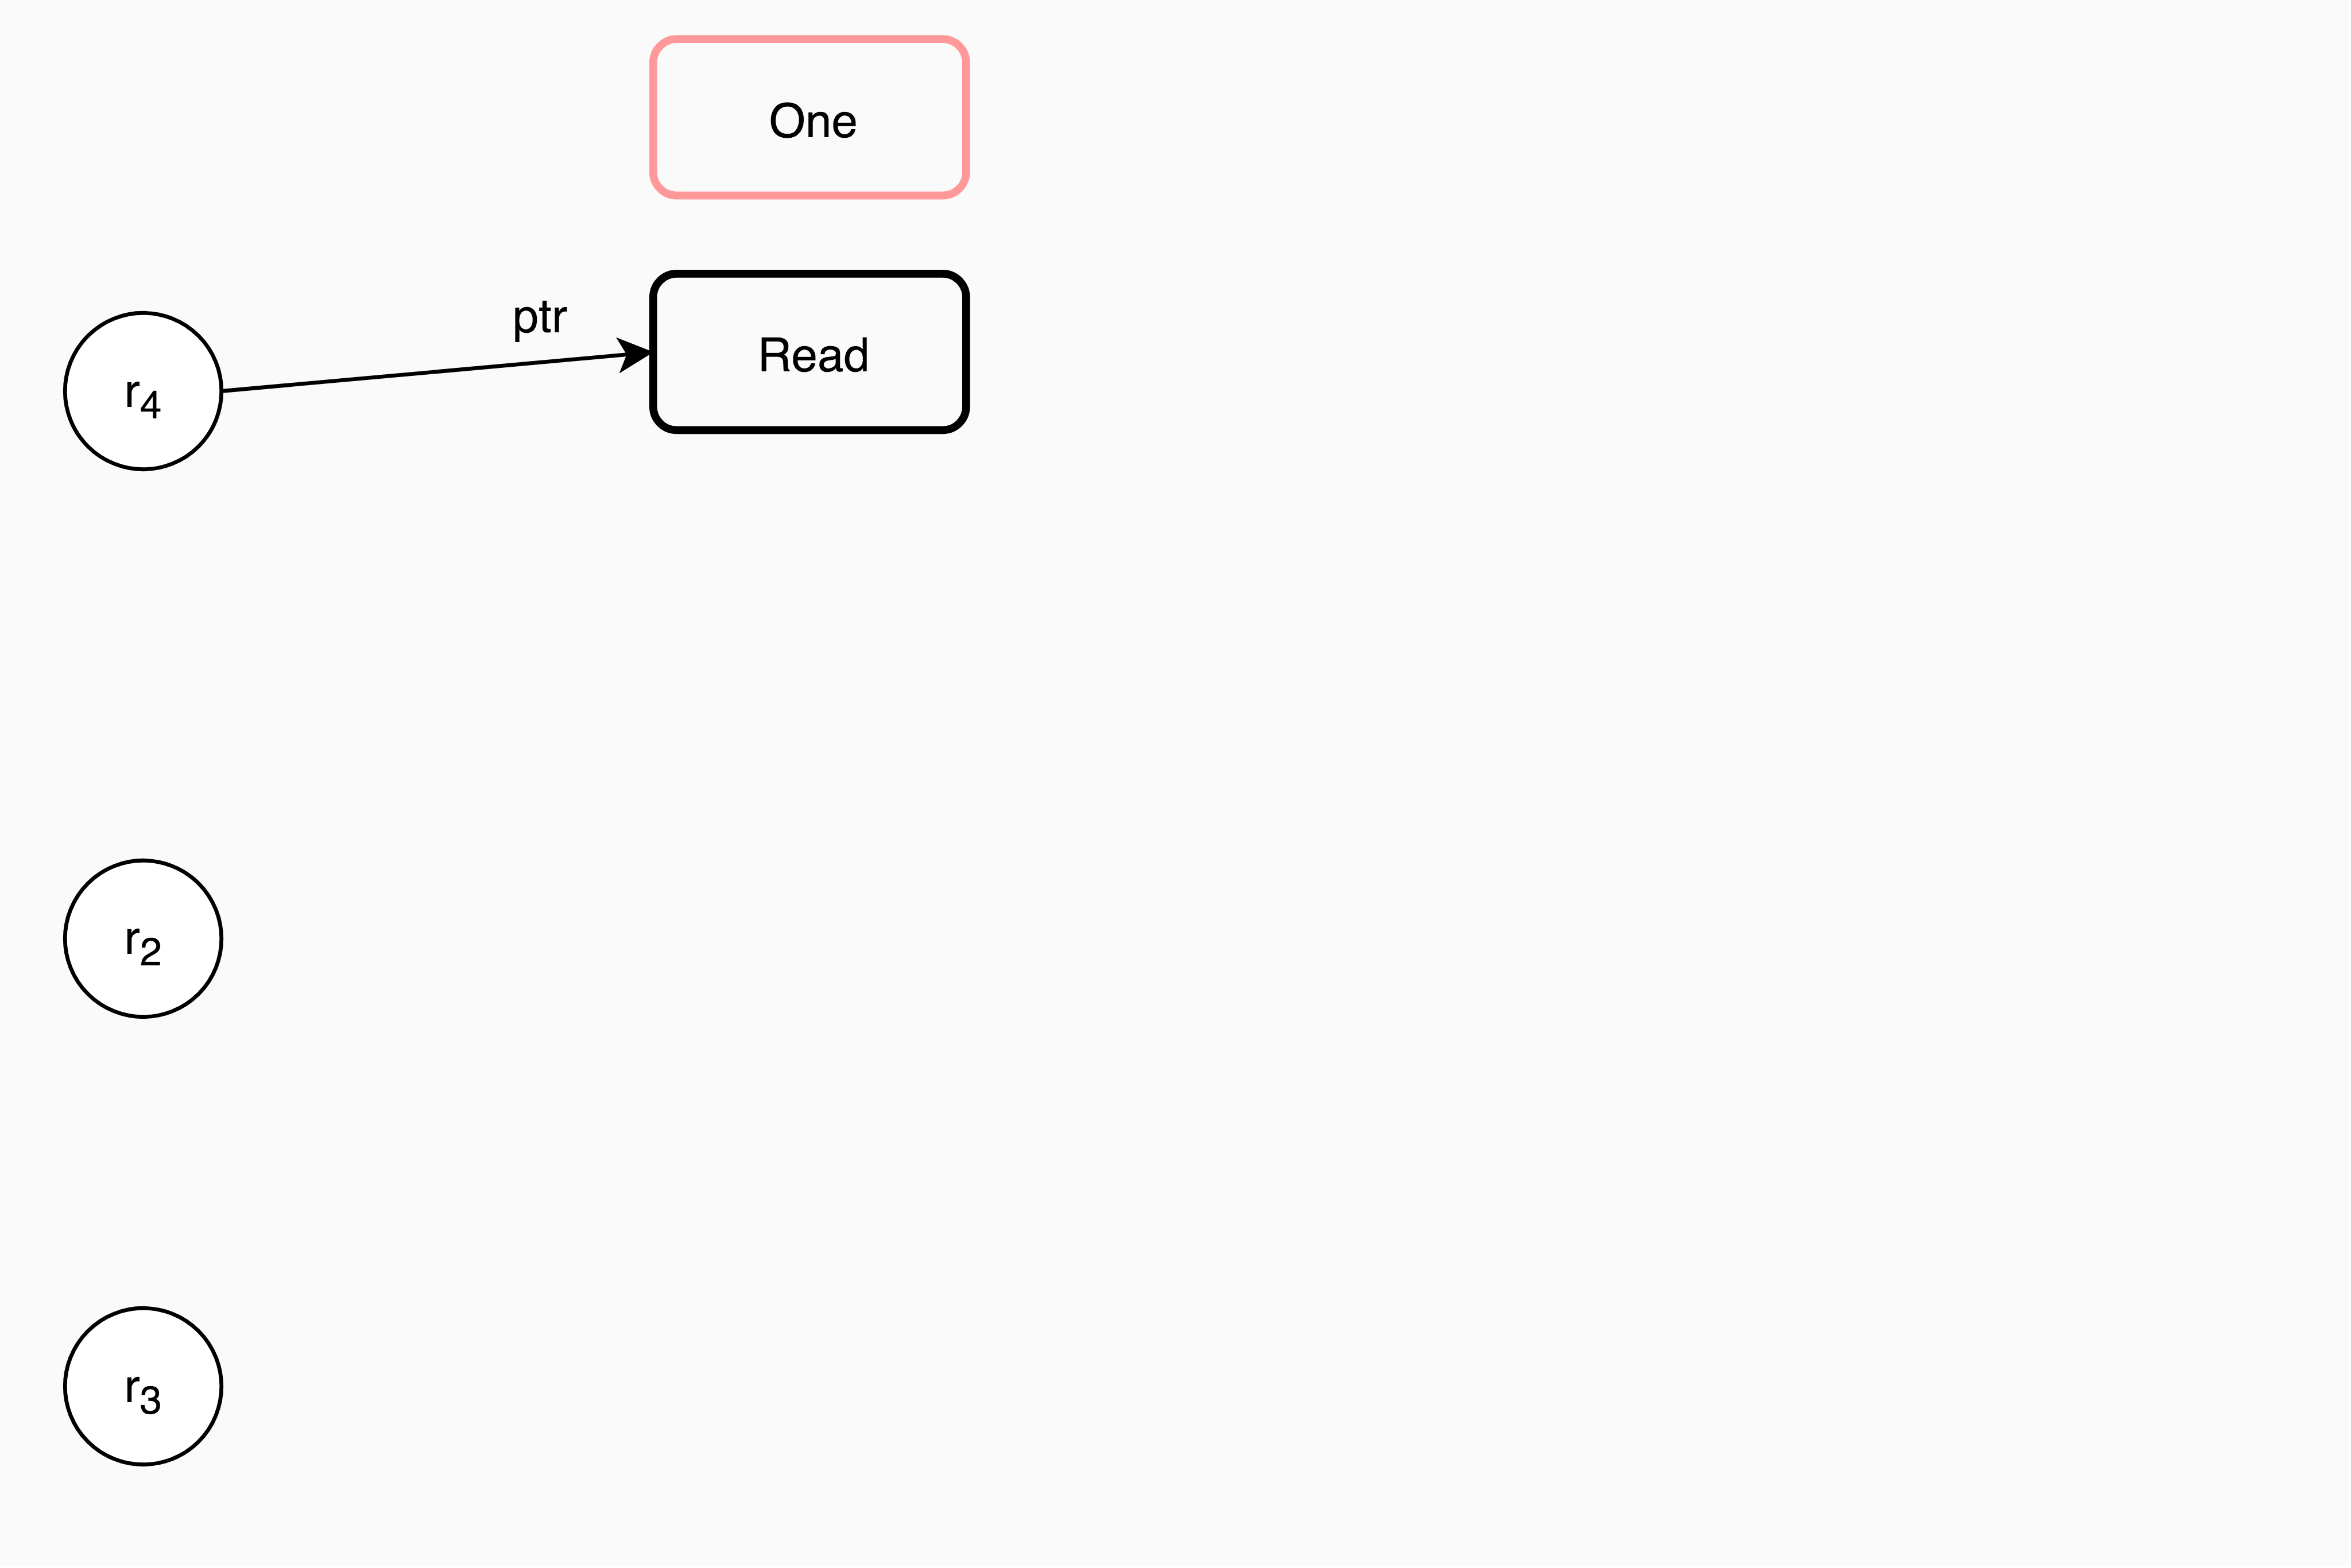
\includegraphics[width=\textwidth]{../figures/example-circuit-3.png}
  	\end{figure}
  \end{frame}
  \begin{frame}{Timestep execution - Circuit execution example}
  	\begin{figure}
  		\centering
  		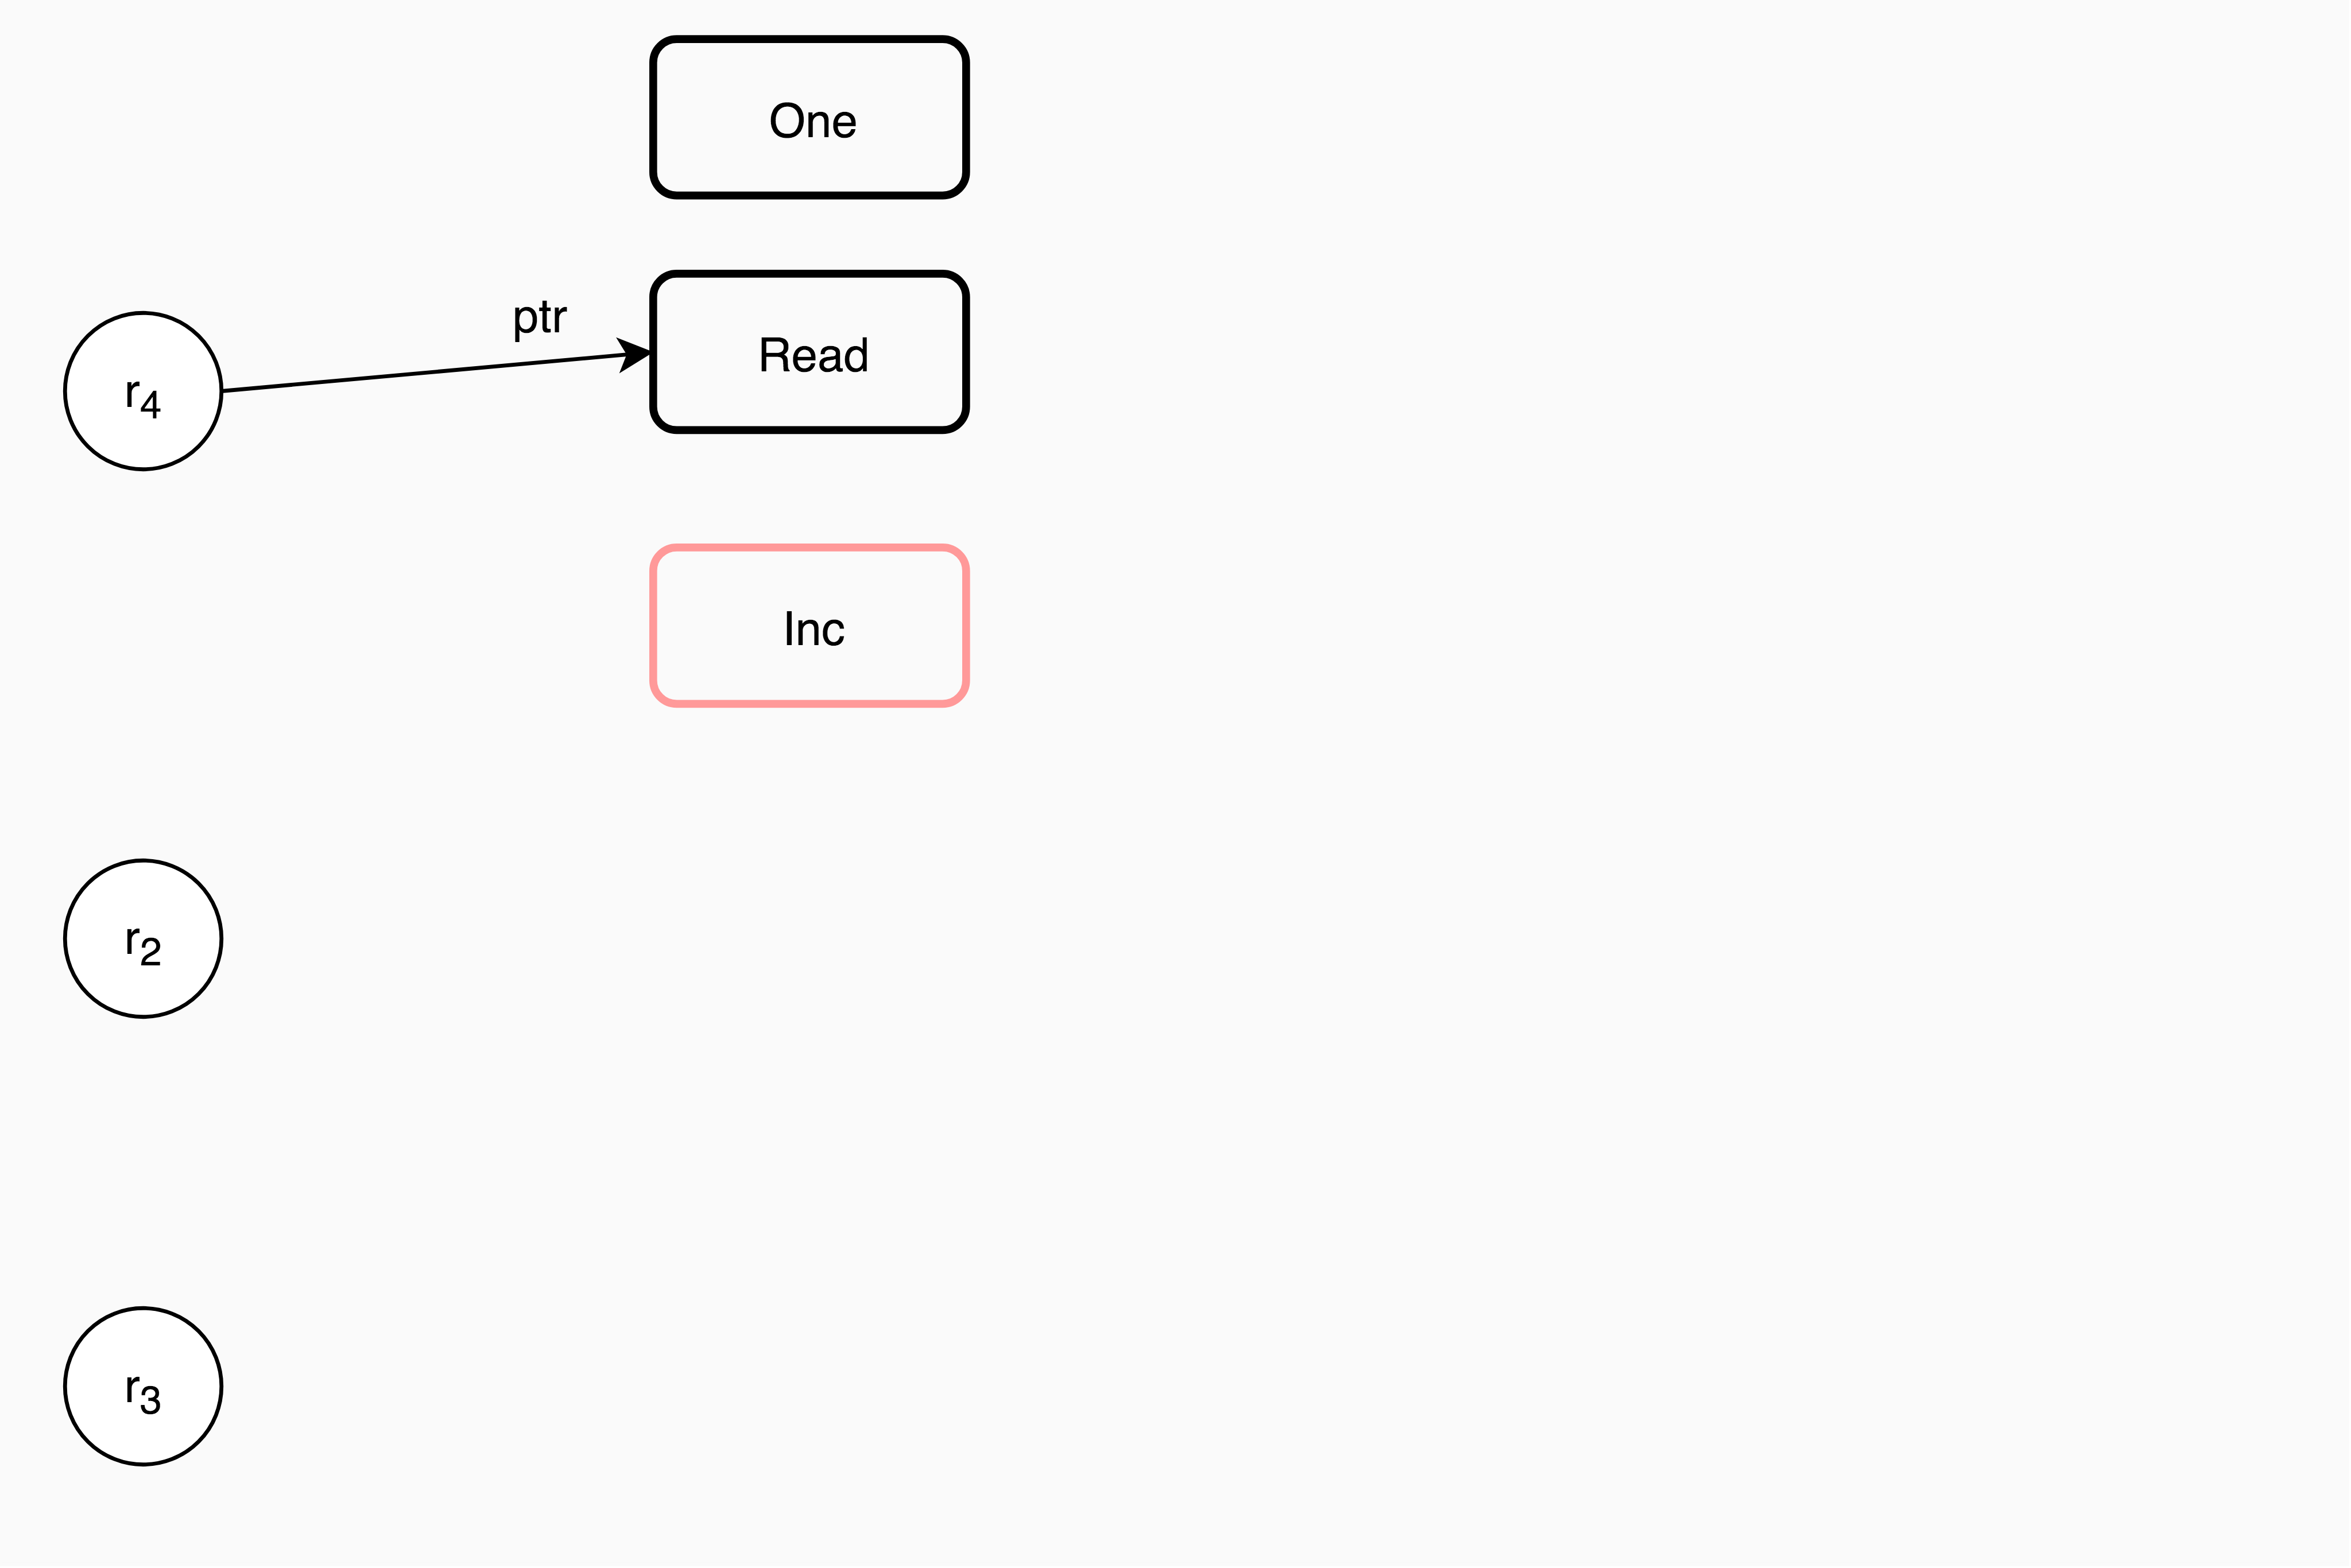
\includegraphics[width=\textwidth]{../figures/example-circuit-4.png}
  	\end{figure}
  \end{frame}
  \begin{frame}{Timestep execution - Circuit execution example}
  	\begin{figure}
  		\centering
  		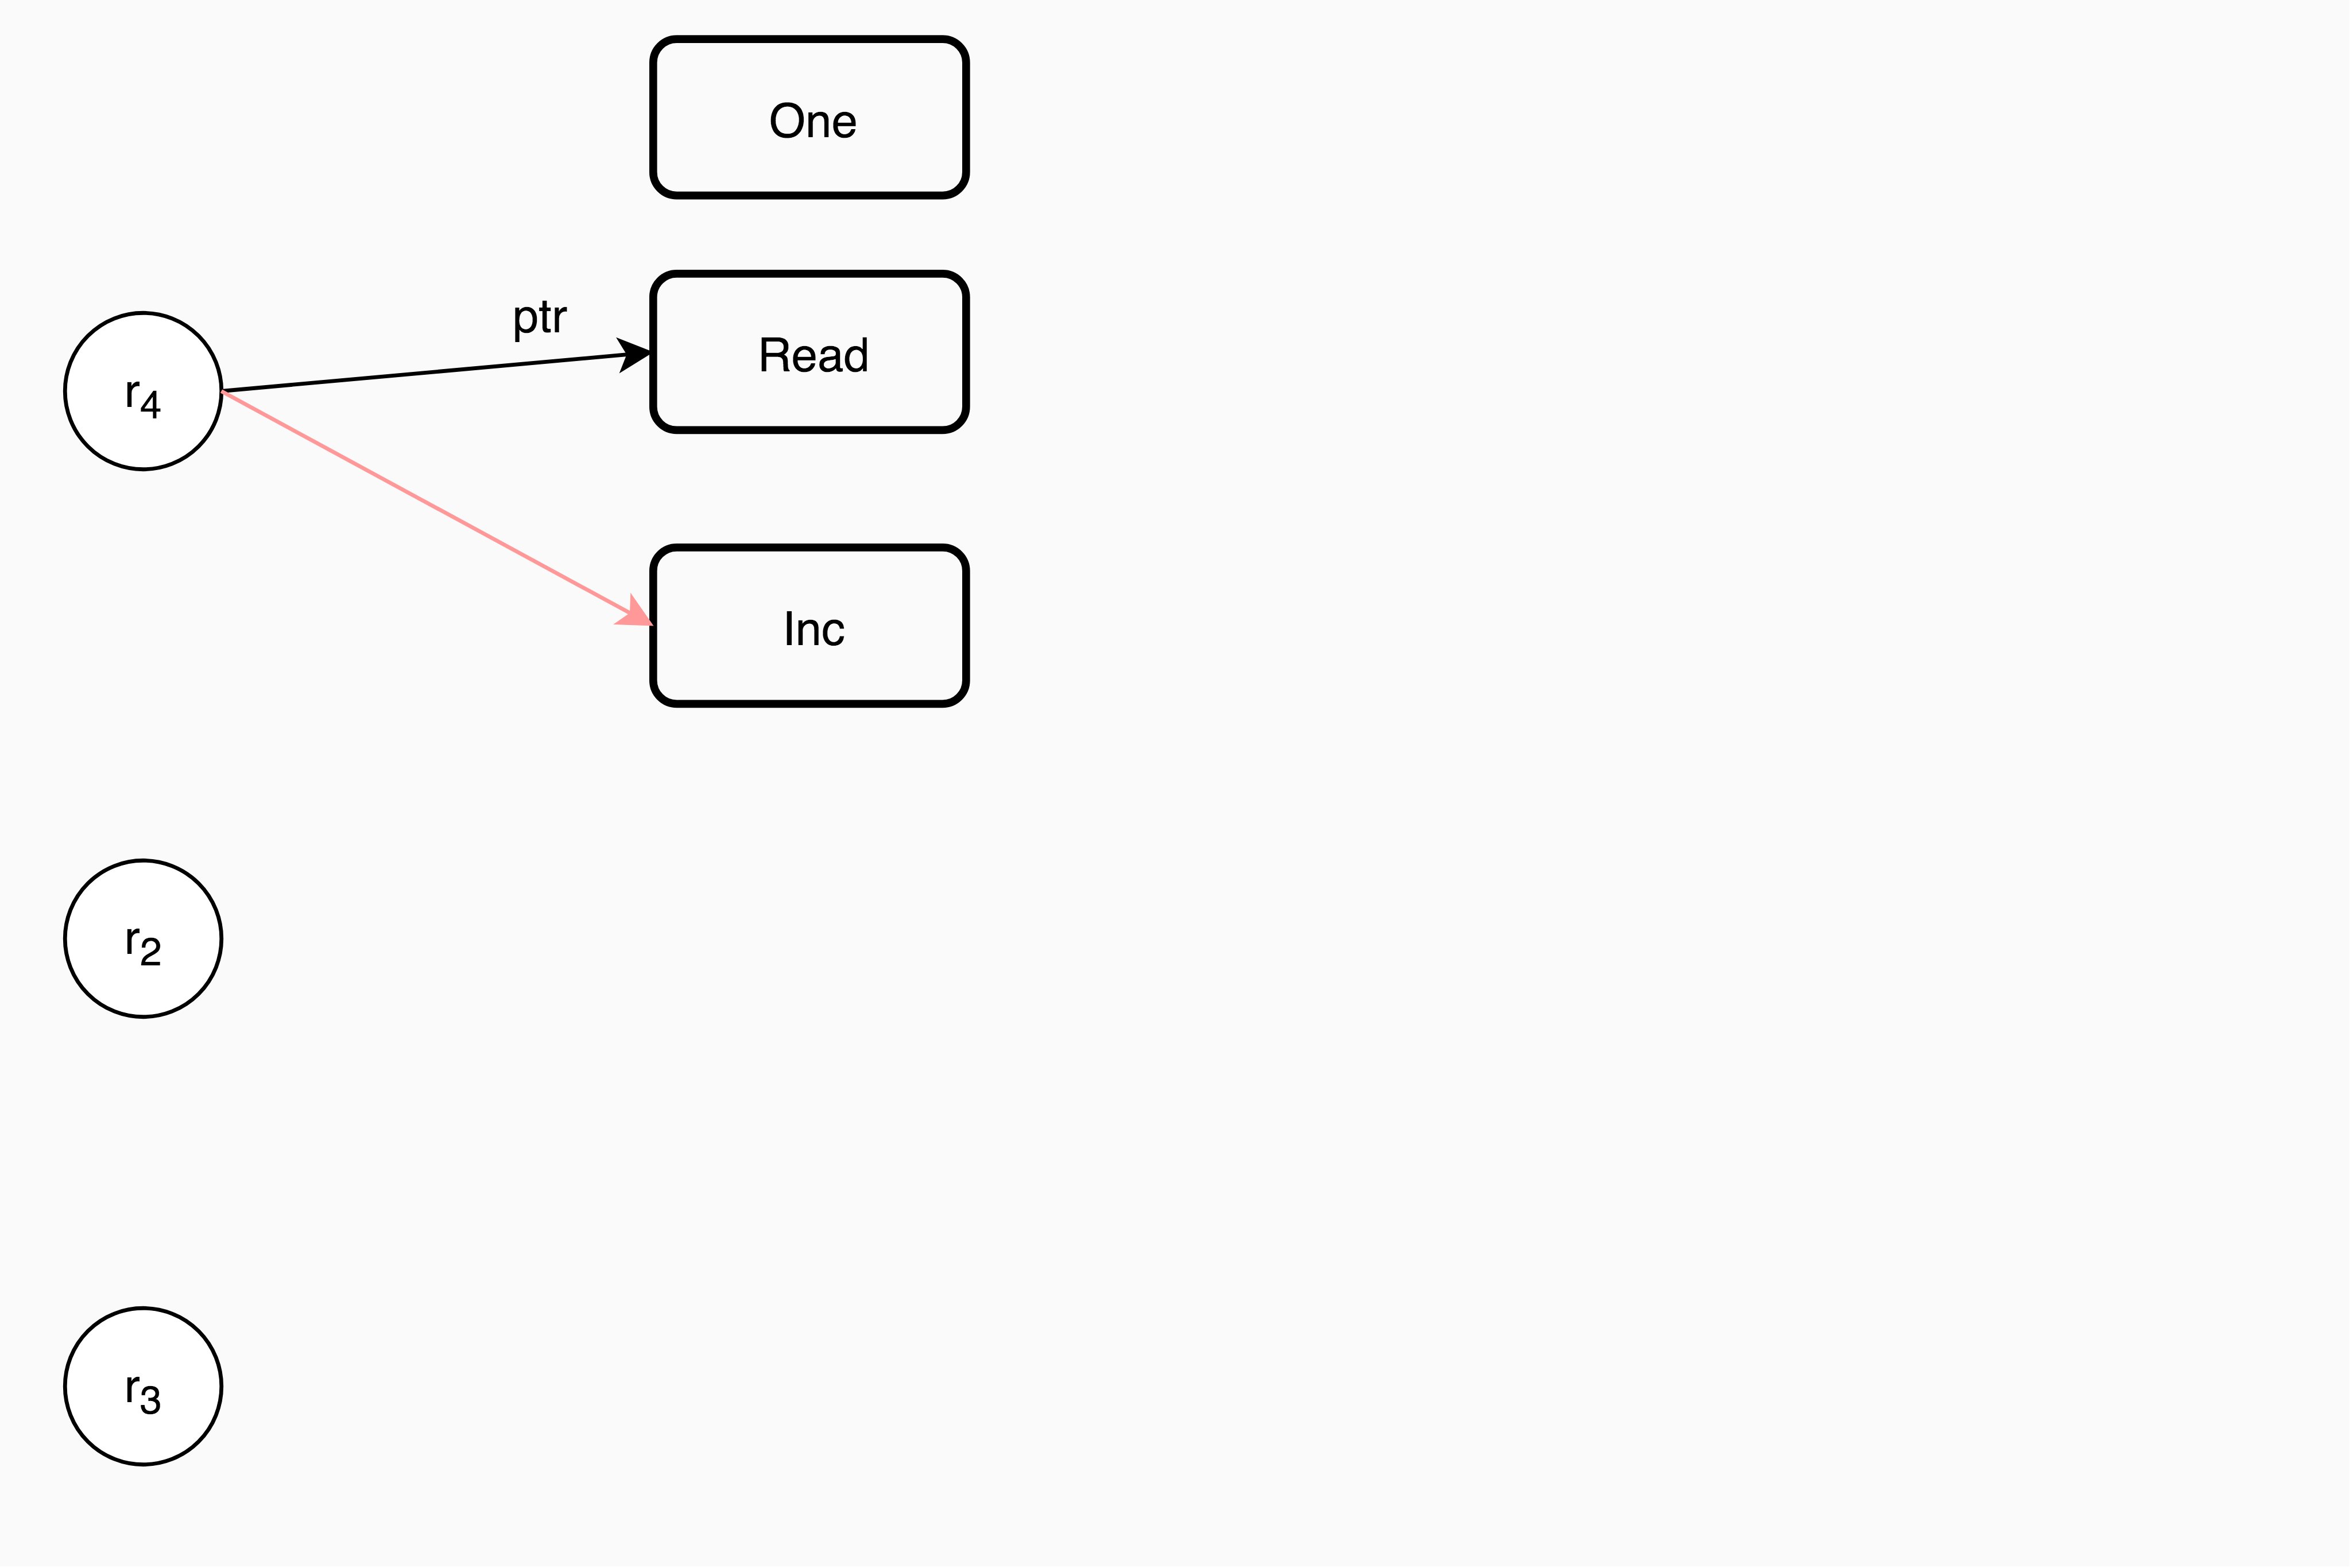
\includegraphics[width=\textwidth]{../figures/example-circuit-5.png}
  	\end{figure}
  \end{frame}
  \begin{frame}{Timestep execution - Circuit execution example}
  	\begin{figure}
  		\centering
  		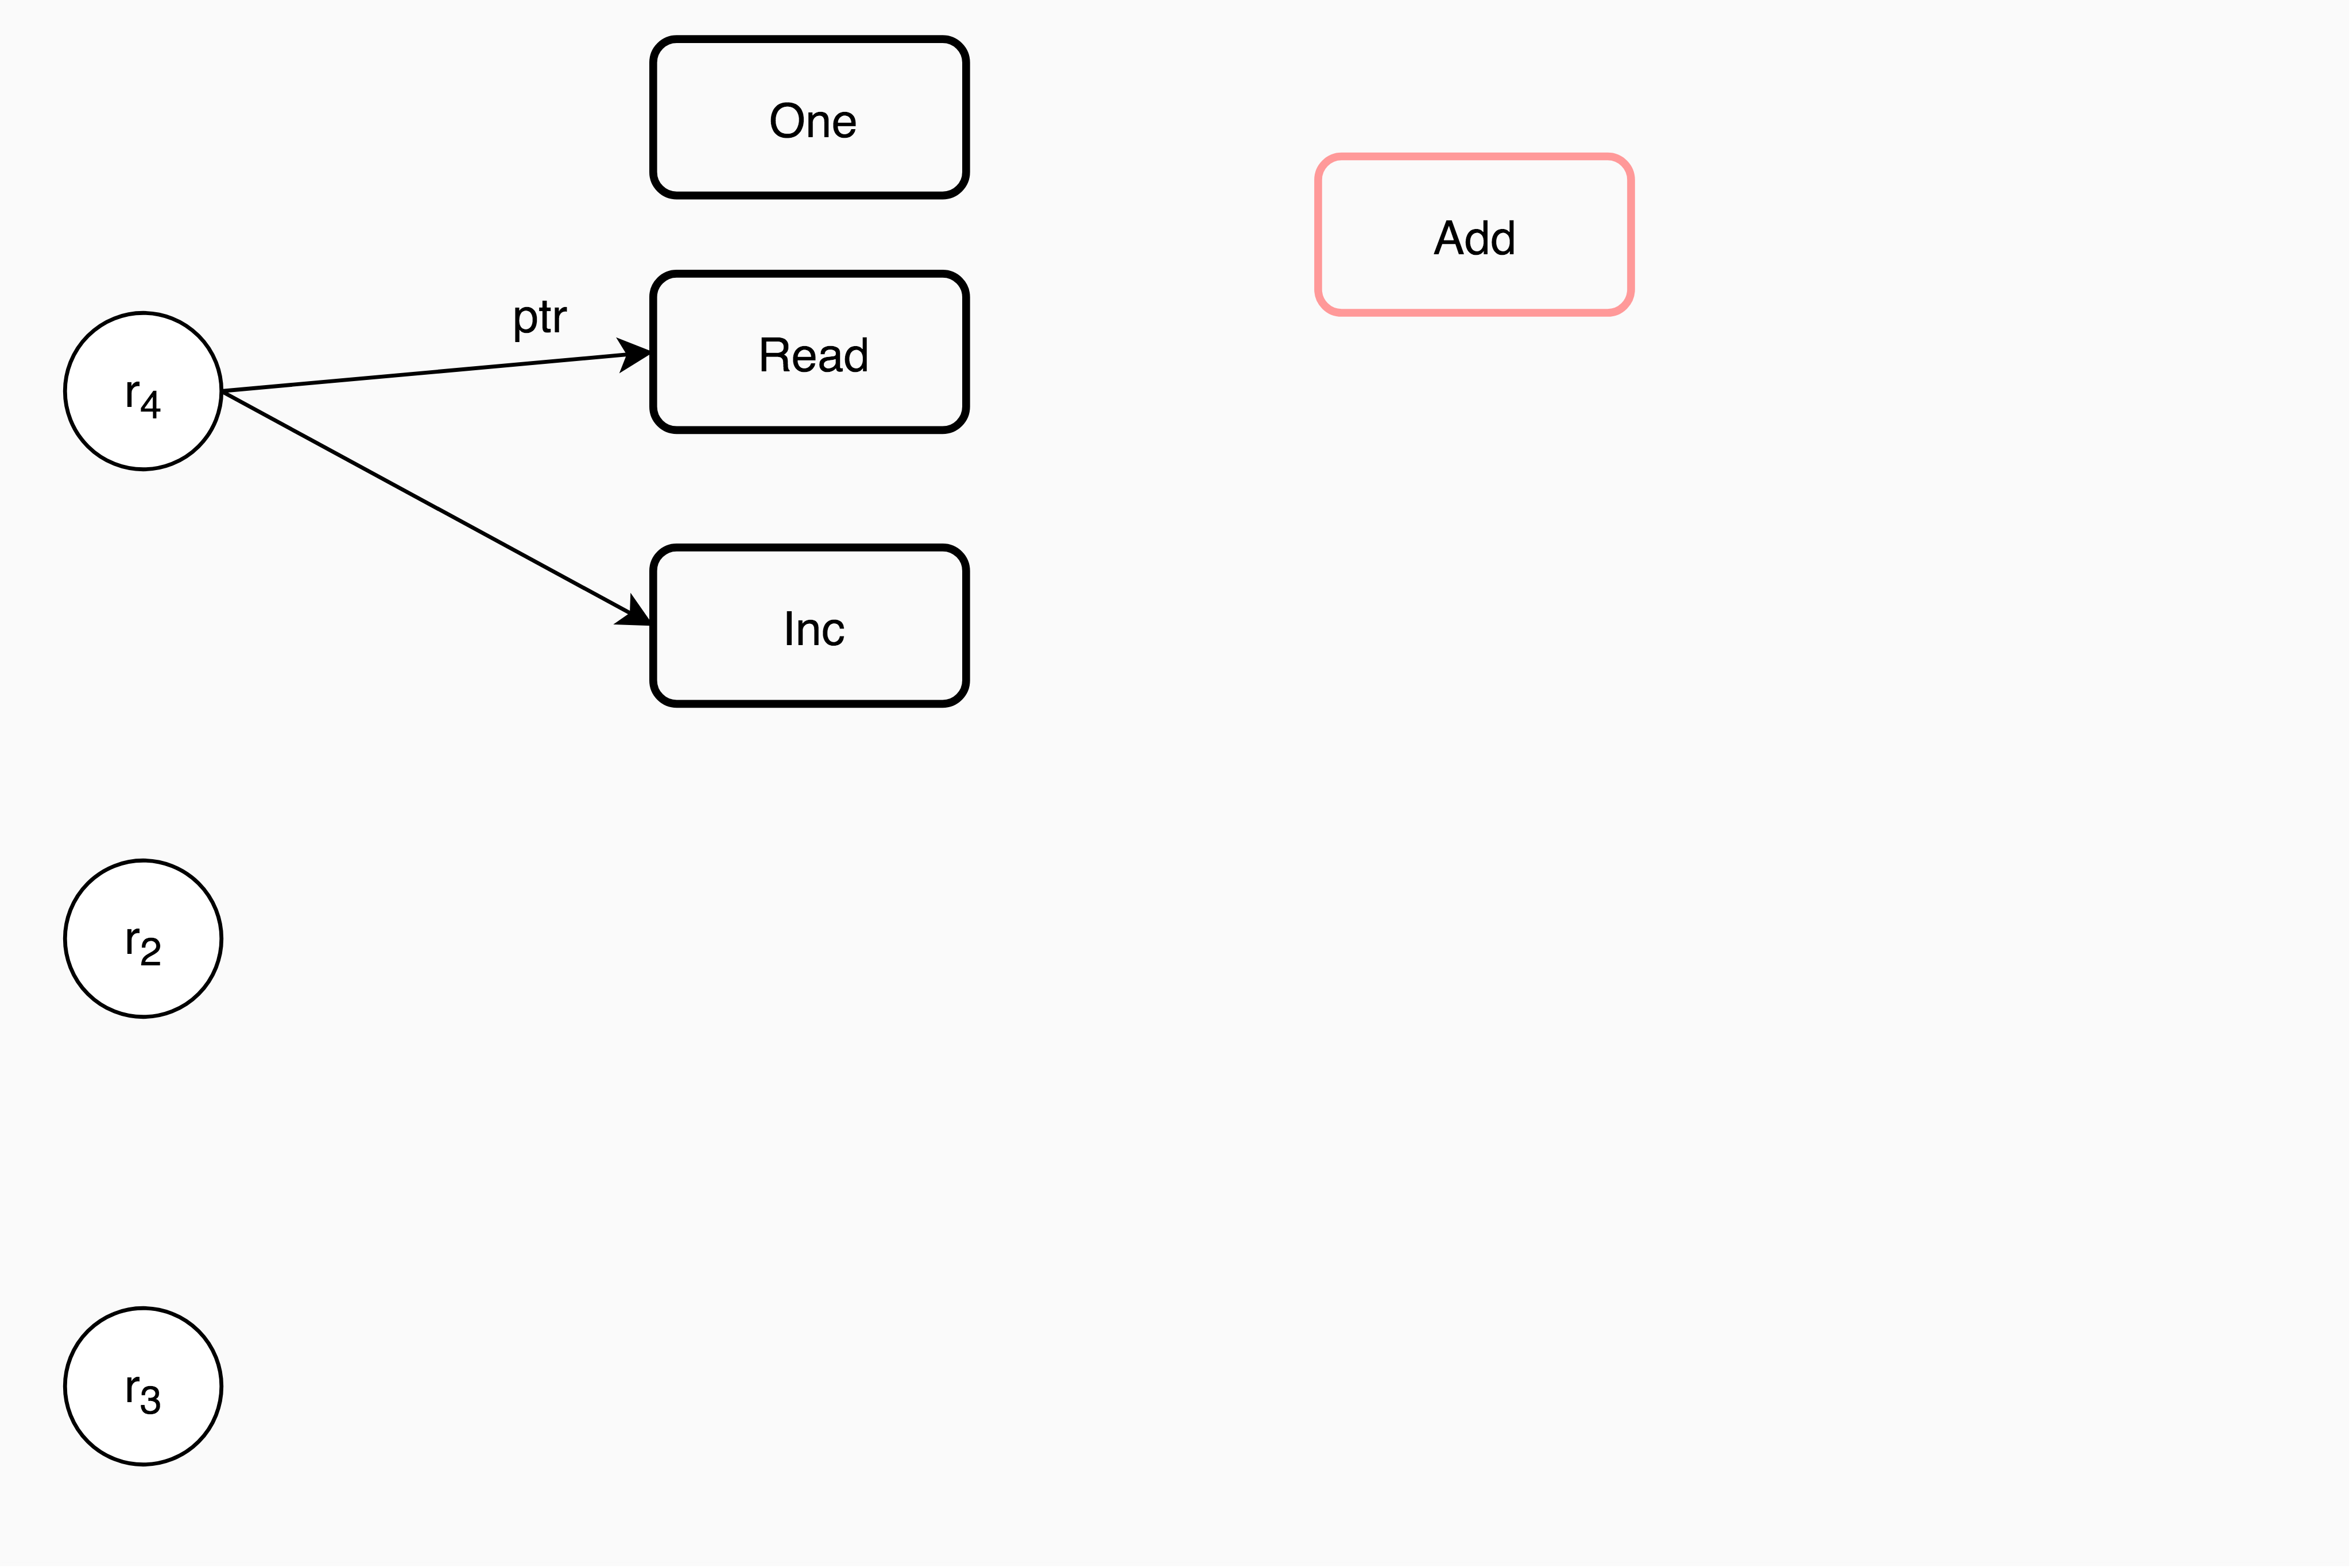
\includegraphics[width=\textwidth]{../figures/example-circuit-6.png}
  	\end{figure}
  \end{frame}
  \begin{frame}{Timestep execution - Circuit execution example}
  	\begin{figure}
  		\centering
  		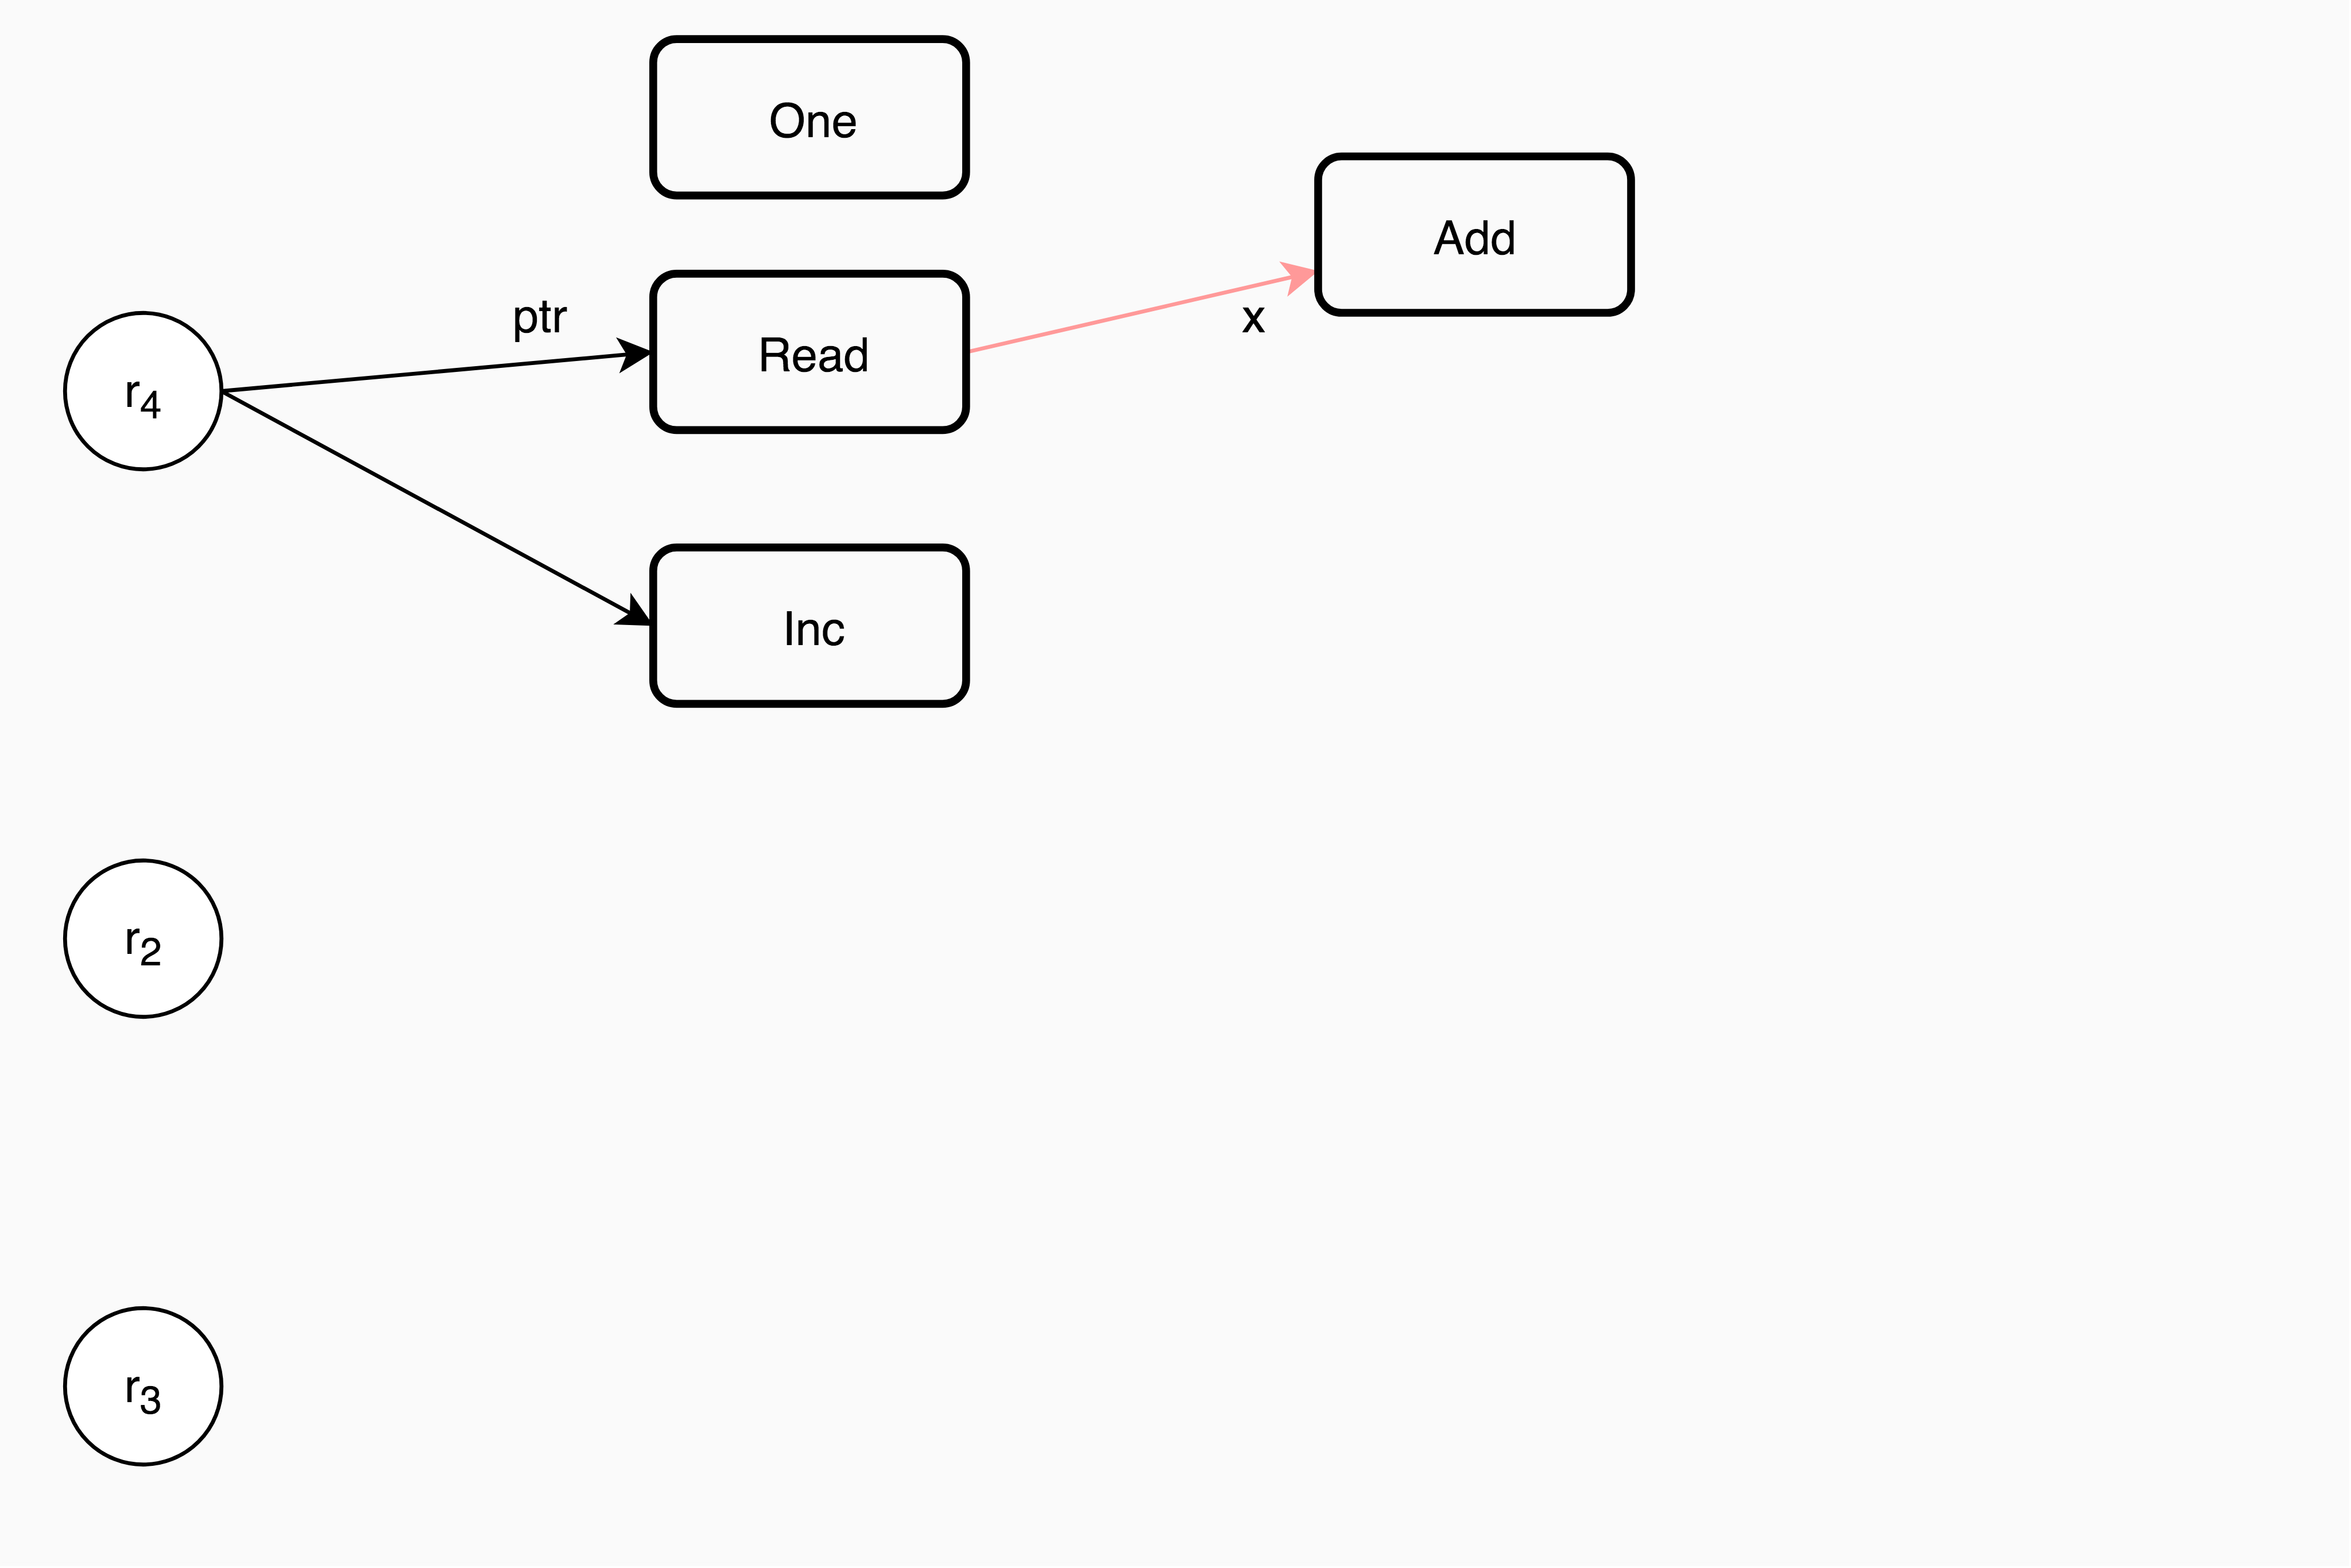
\includegraphics[width=\textwidth]{../figures/example-circuit-7.png}
  	\end{figure}
  \end{frame}
  \begin{frame}{Timestep execution - Circuit execution example}
  	\begin{figure}
  		\centering
  		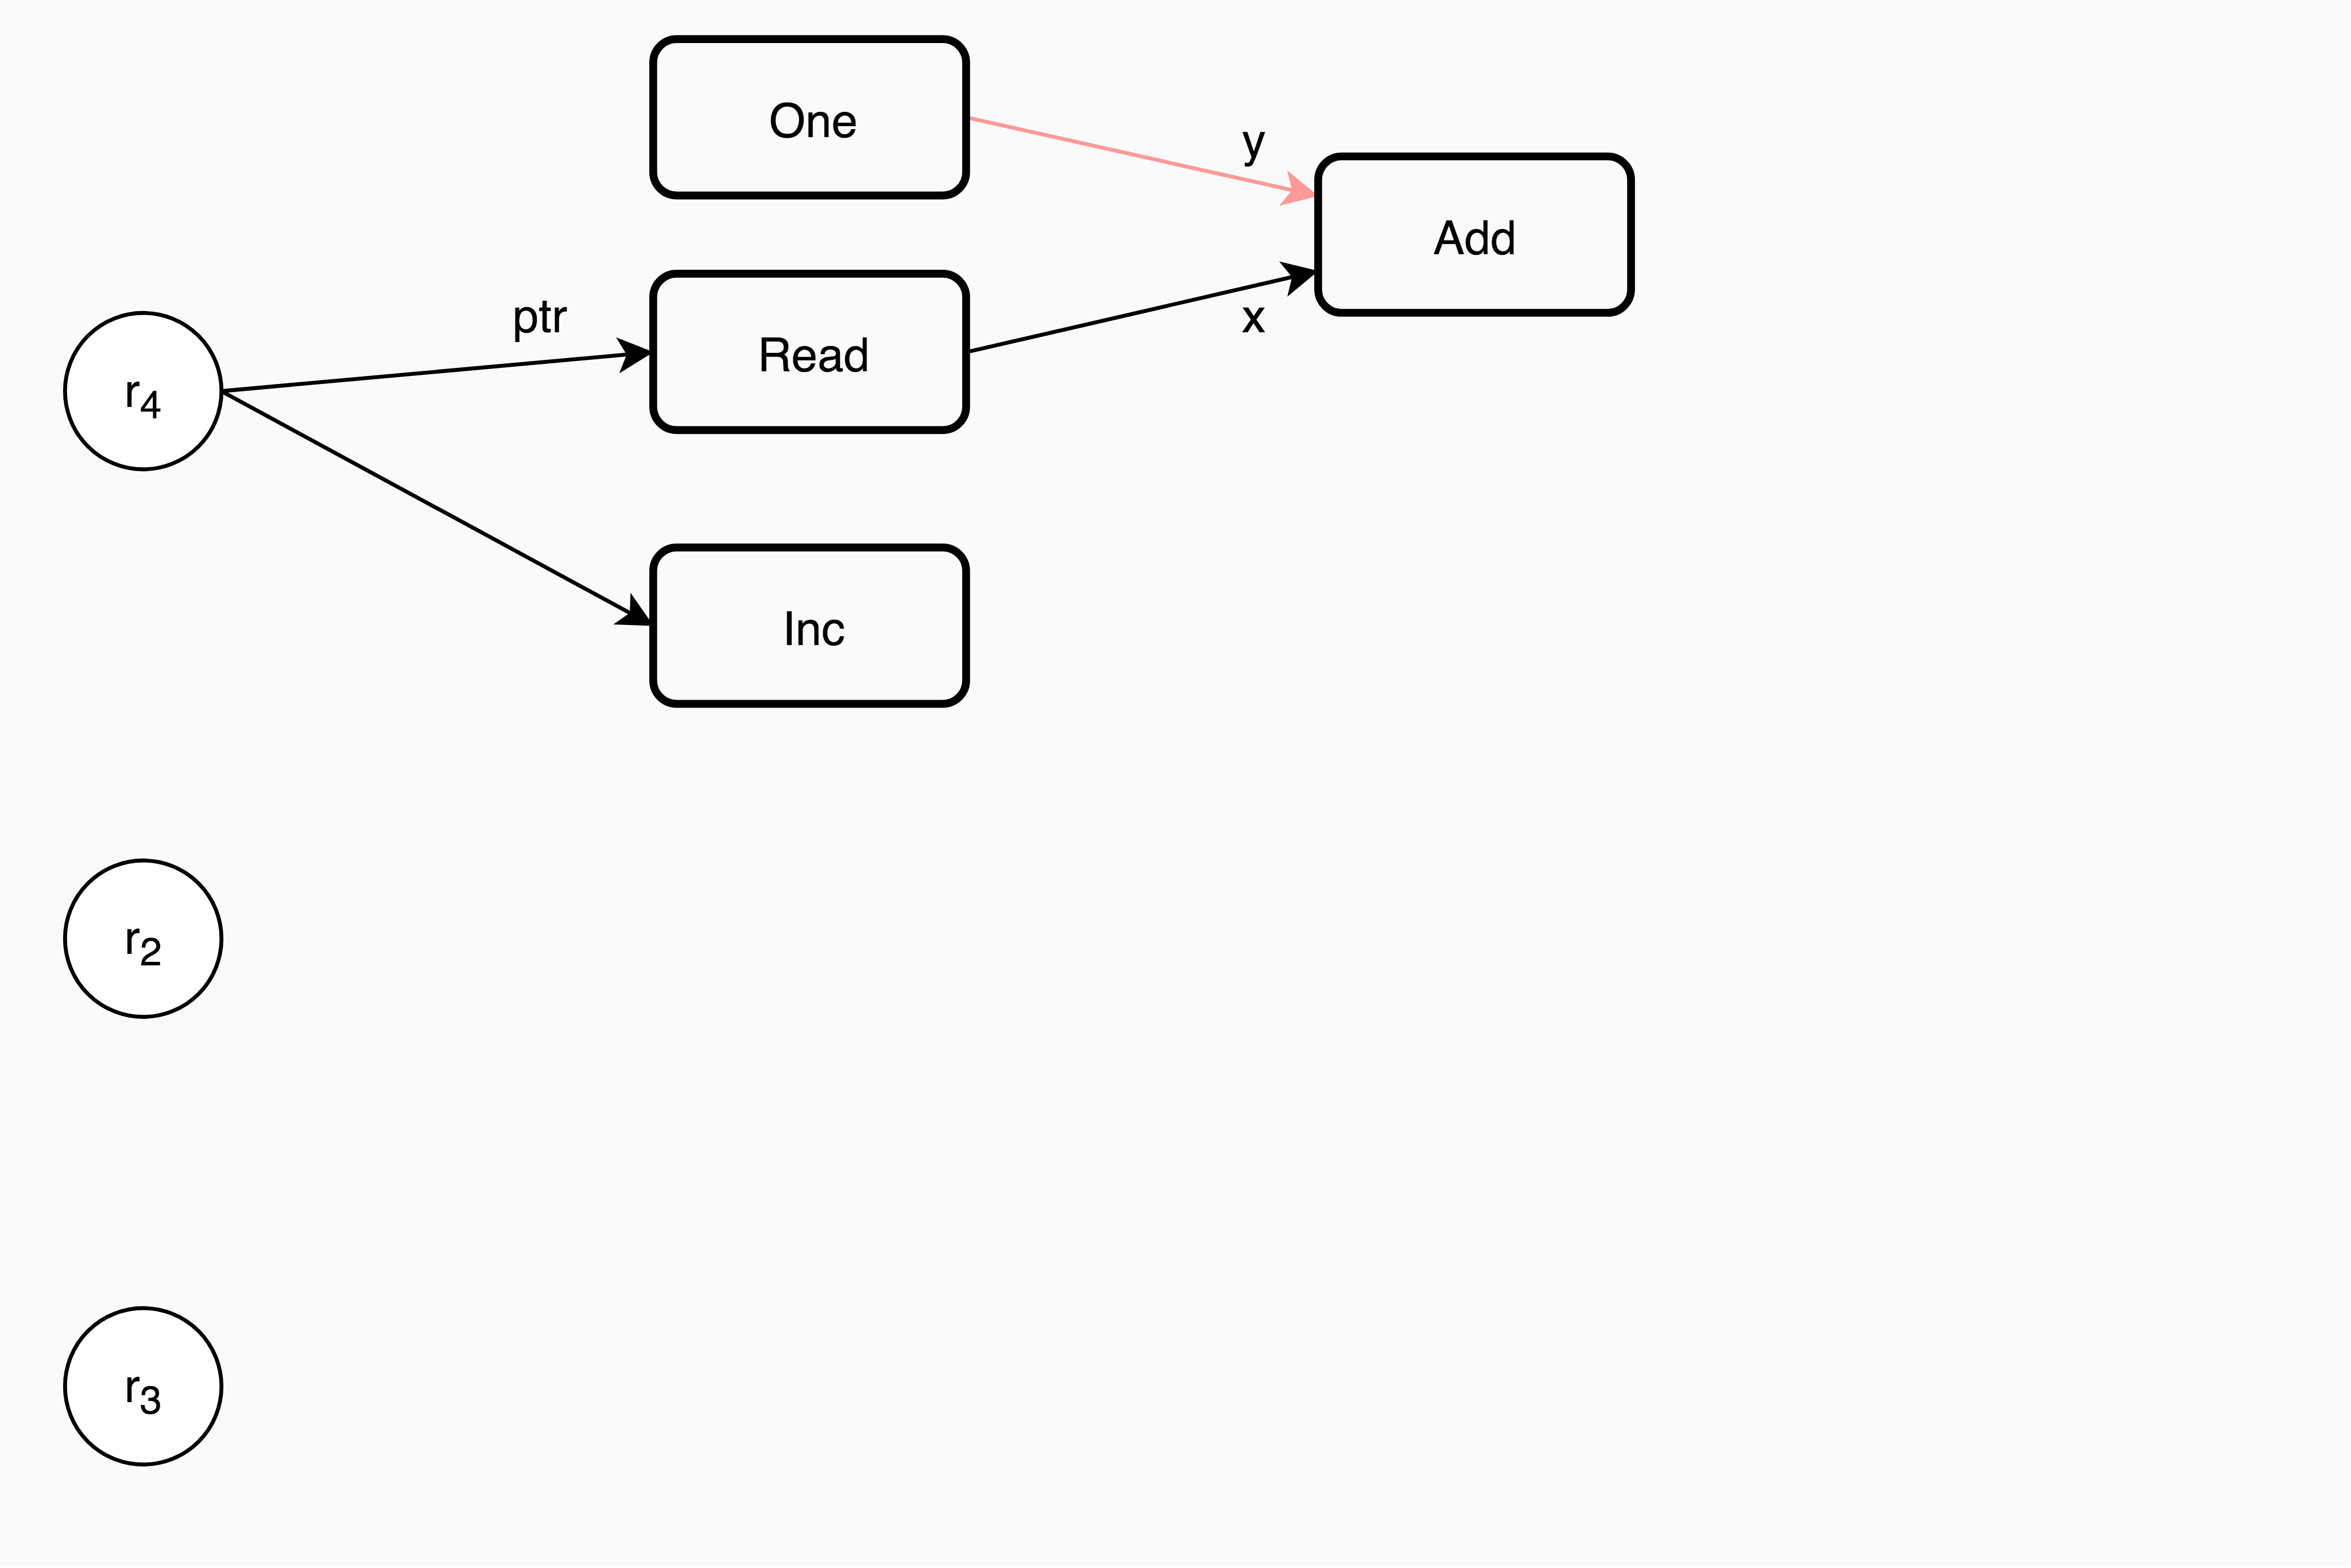
\includegraphics[width=\textwidth]{../figures/example-circuit-8.png}
  	\end{figure}
  \end{frame}
  \begin{frame}{Timestep execution - Circuit execution example}
  	\begin{figure}
  		\centering
  		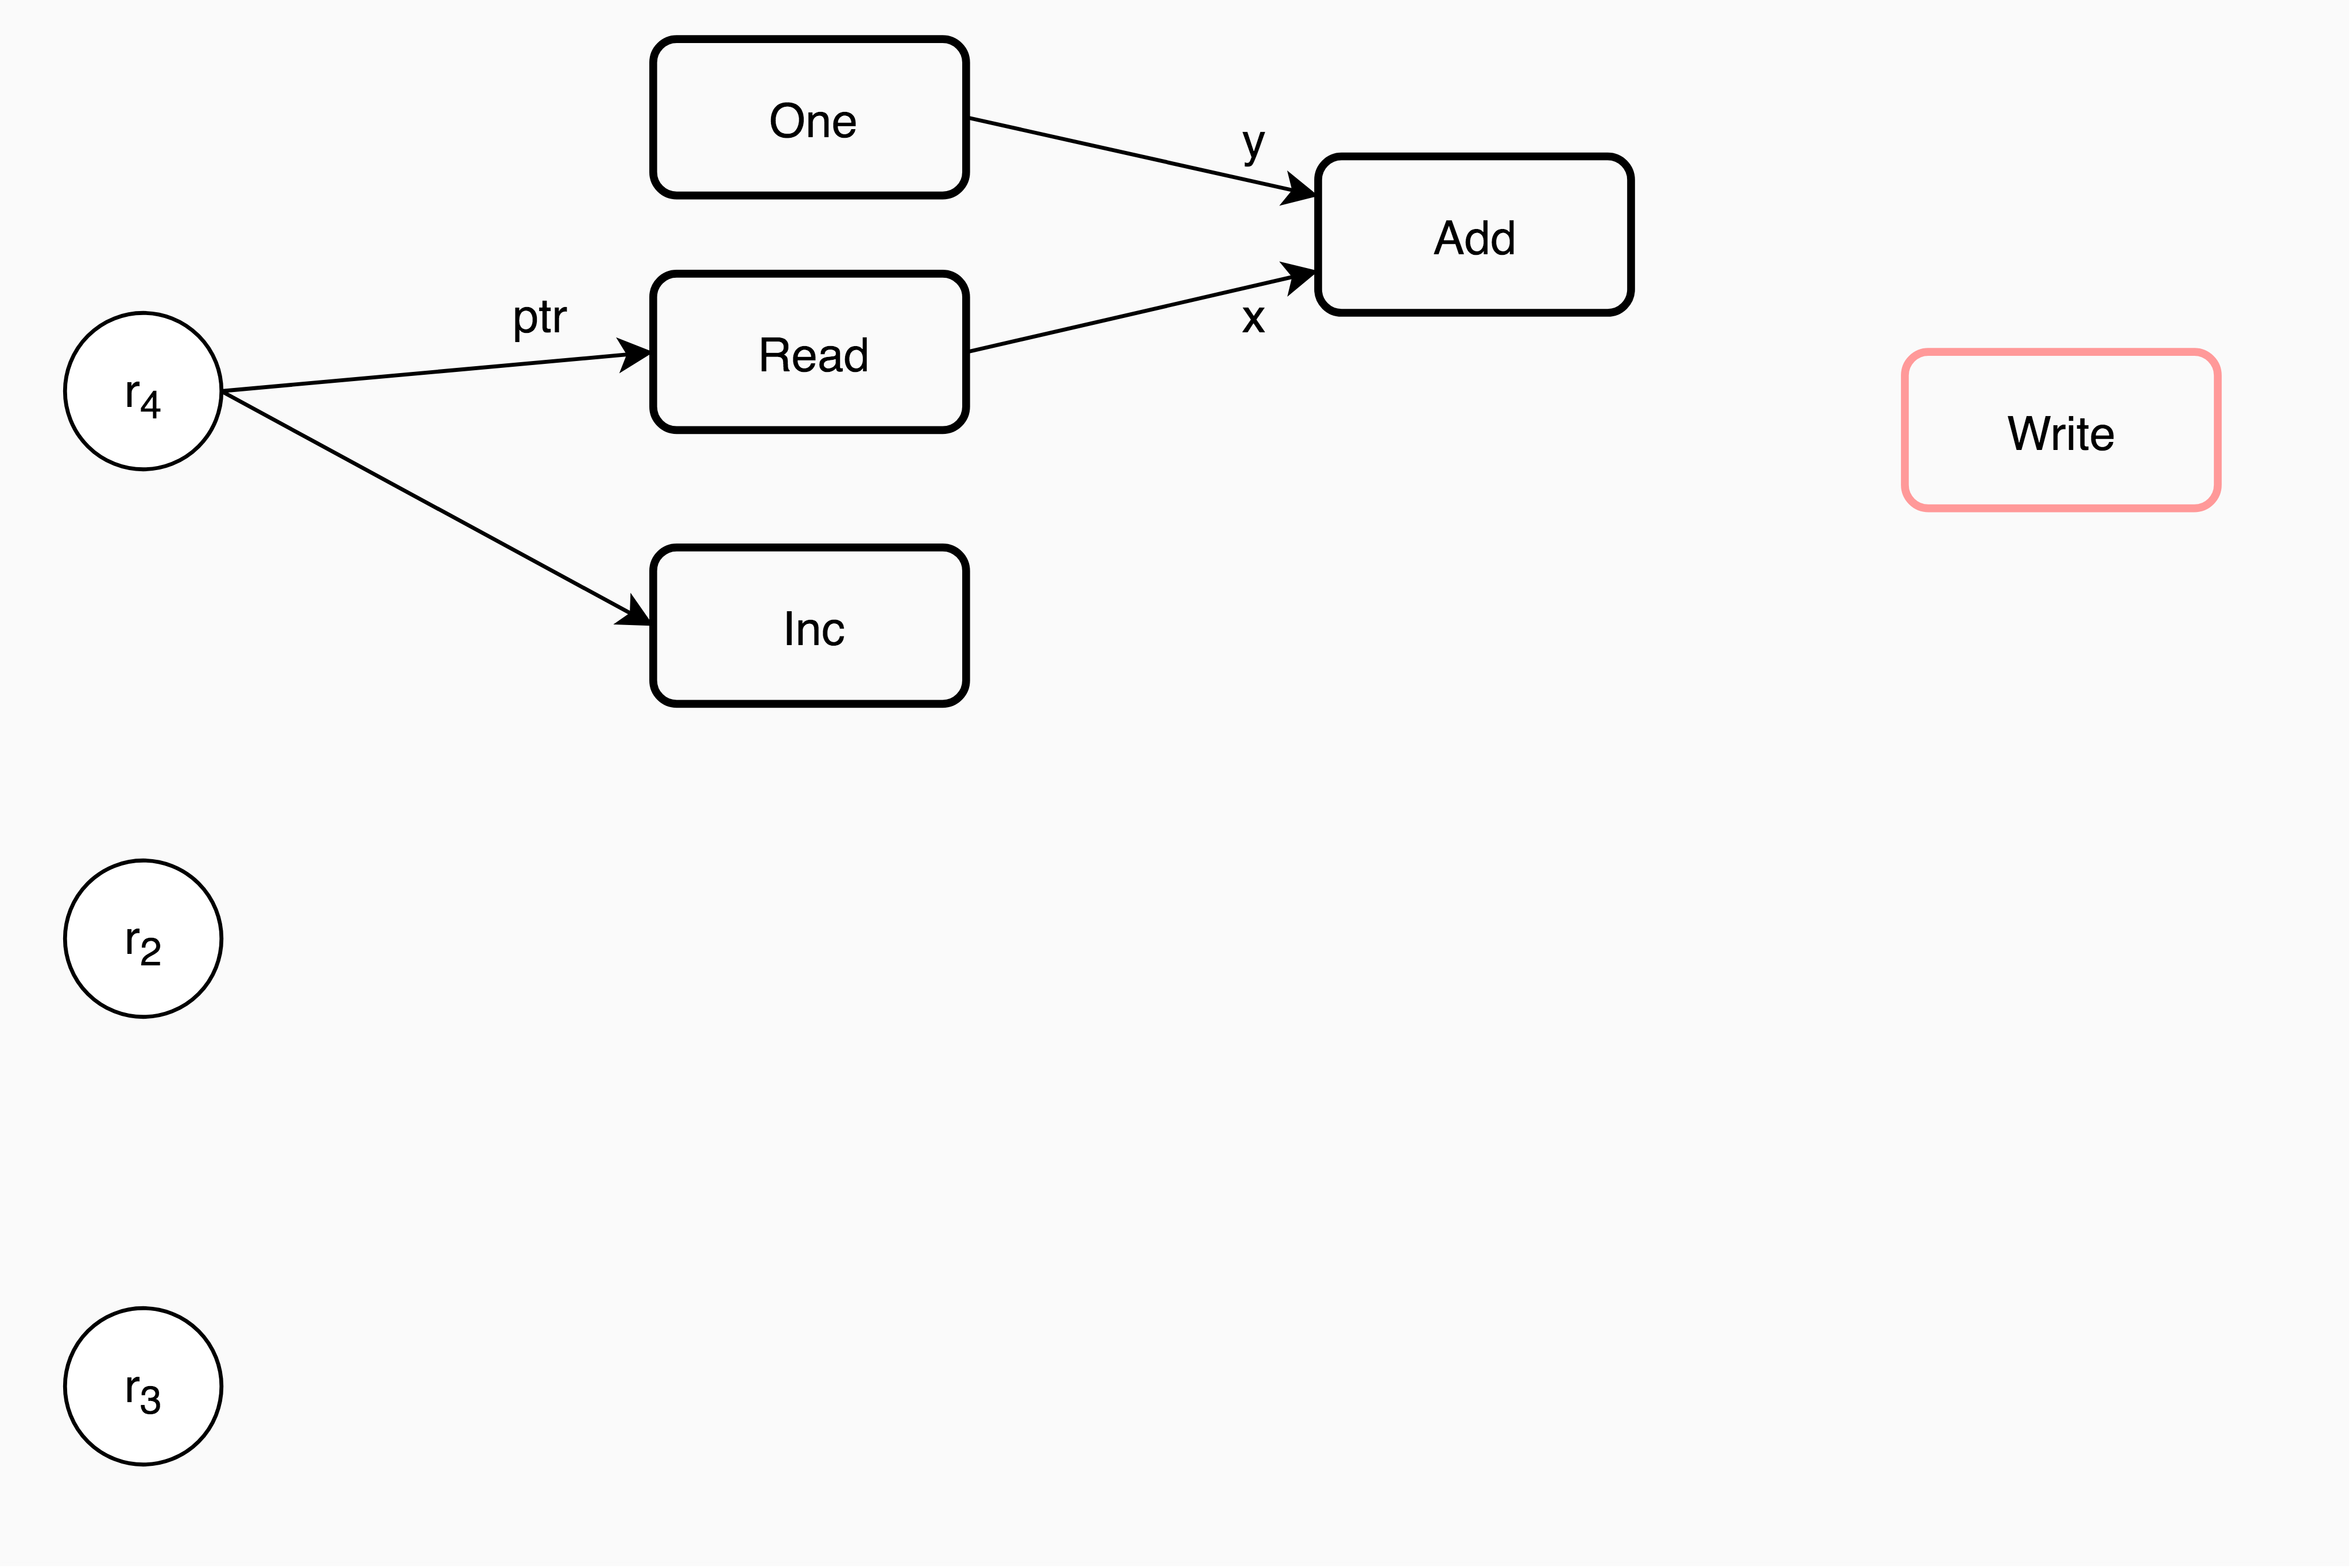
\includegraphics[width=\textwidth]{../figures/example-circuit-9.png}
  	\end{figure}
  \end{frame}
  \begin{frame}{Timestep execution - Circuit execution example}
  	\begin{figure}
  		\centering
  		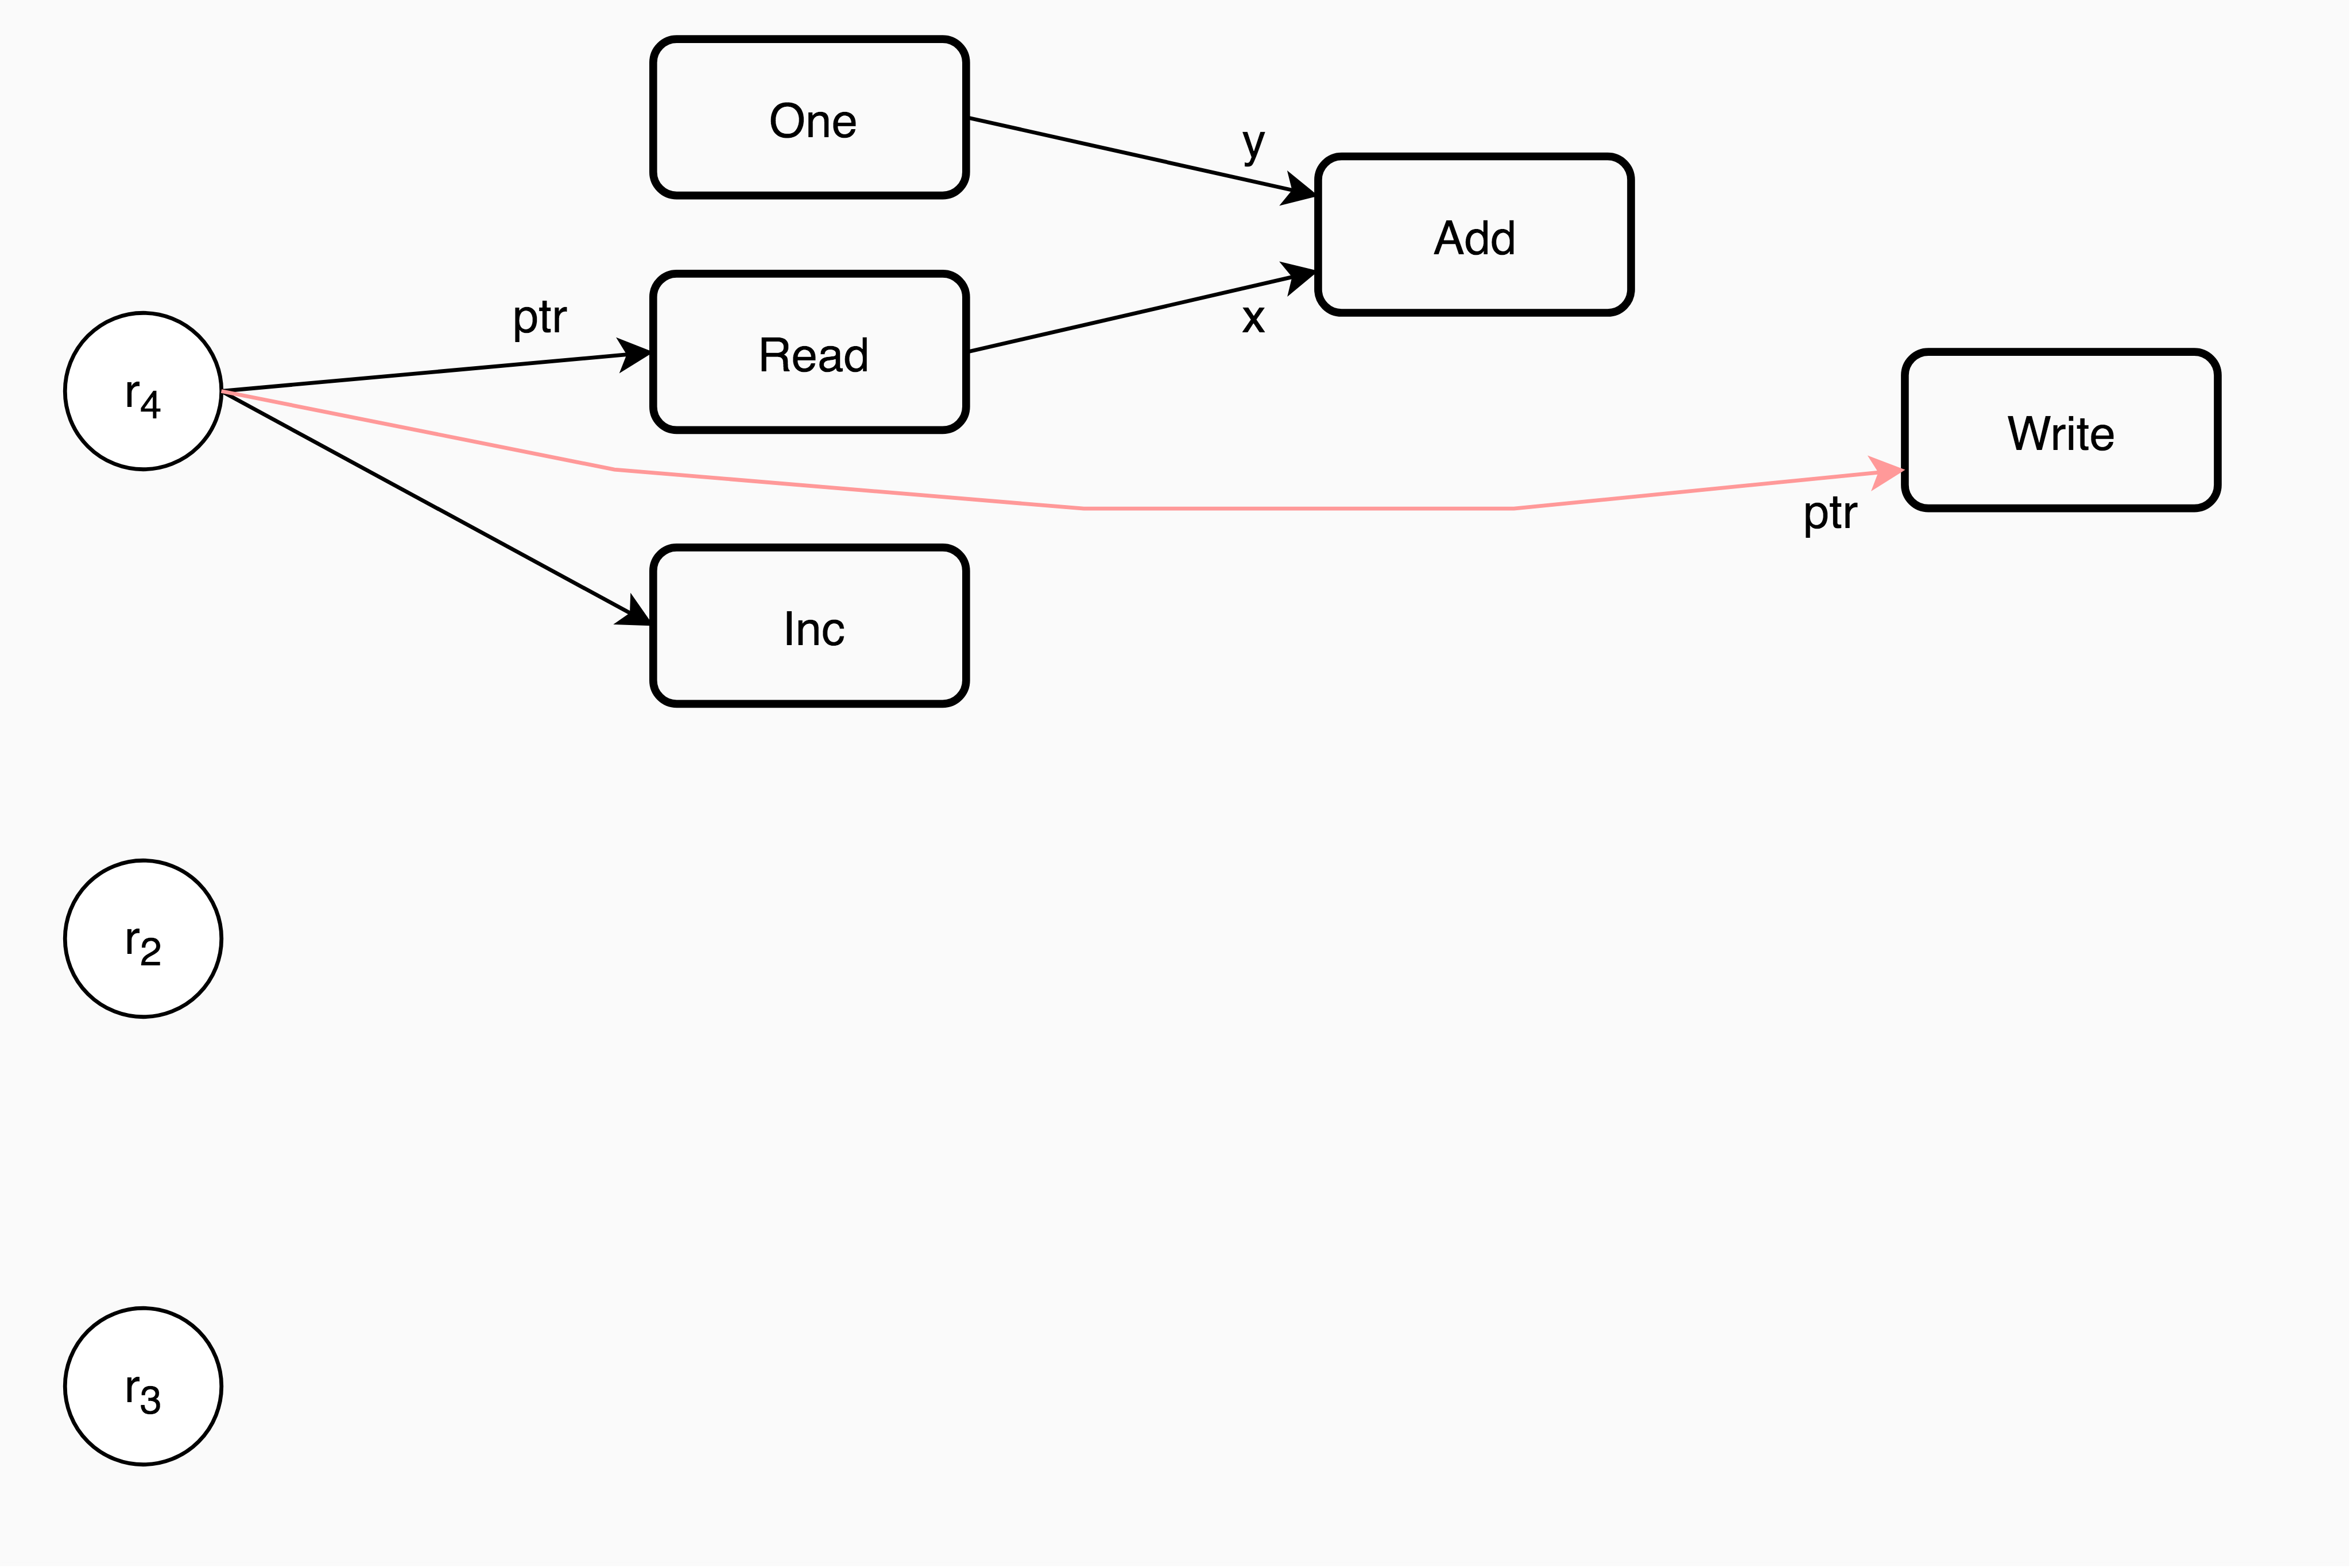
\includegraphics[width=\textwidth]{../figures/example-circuit-10.png}
  	\end{figure}
  \end{frame}
  \begin{frame}{Timestep execution - Circuit execution example}
  	\begin{figure}
  		\centering
  		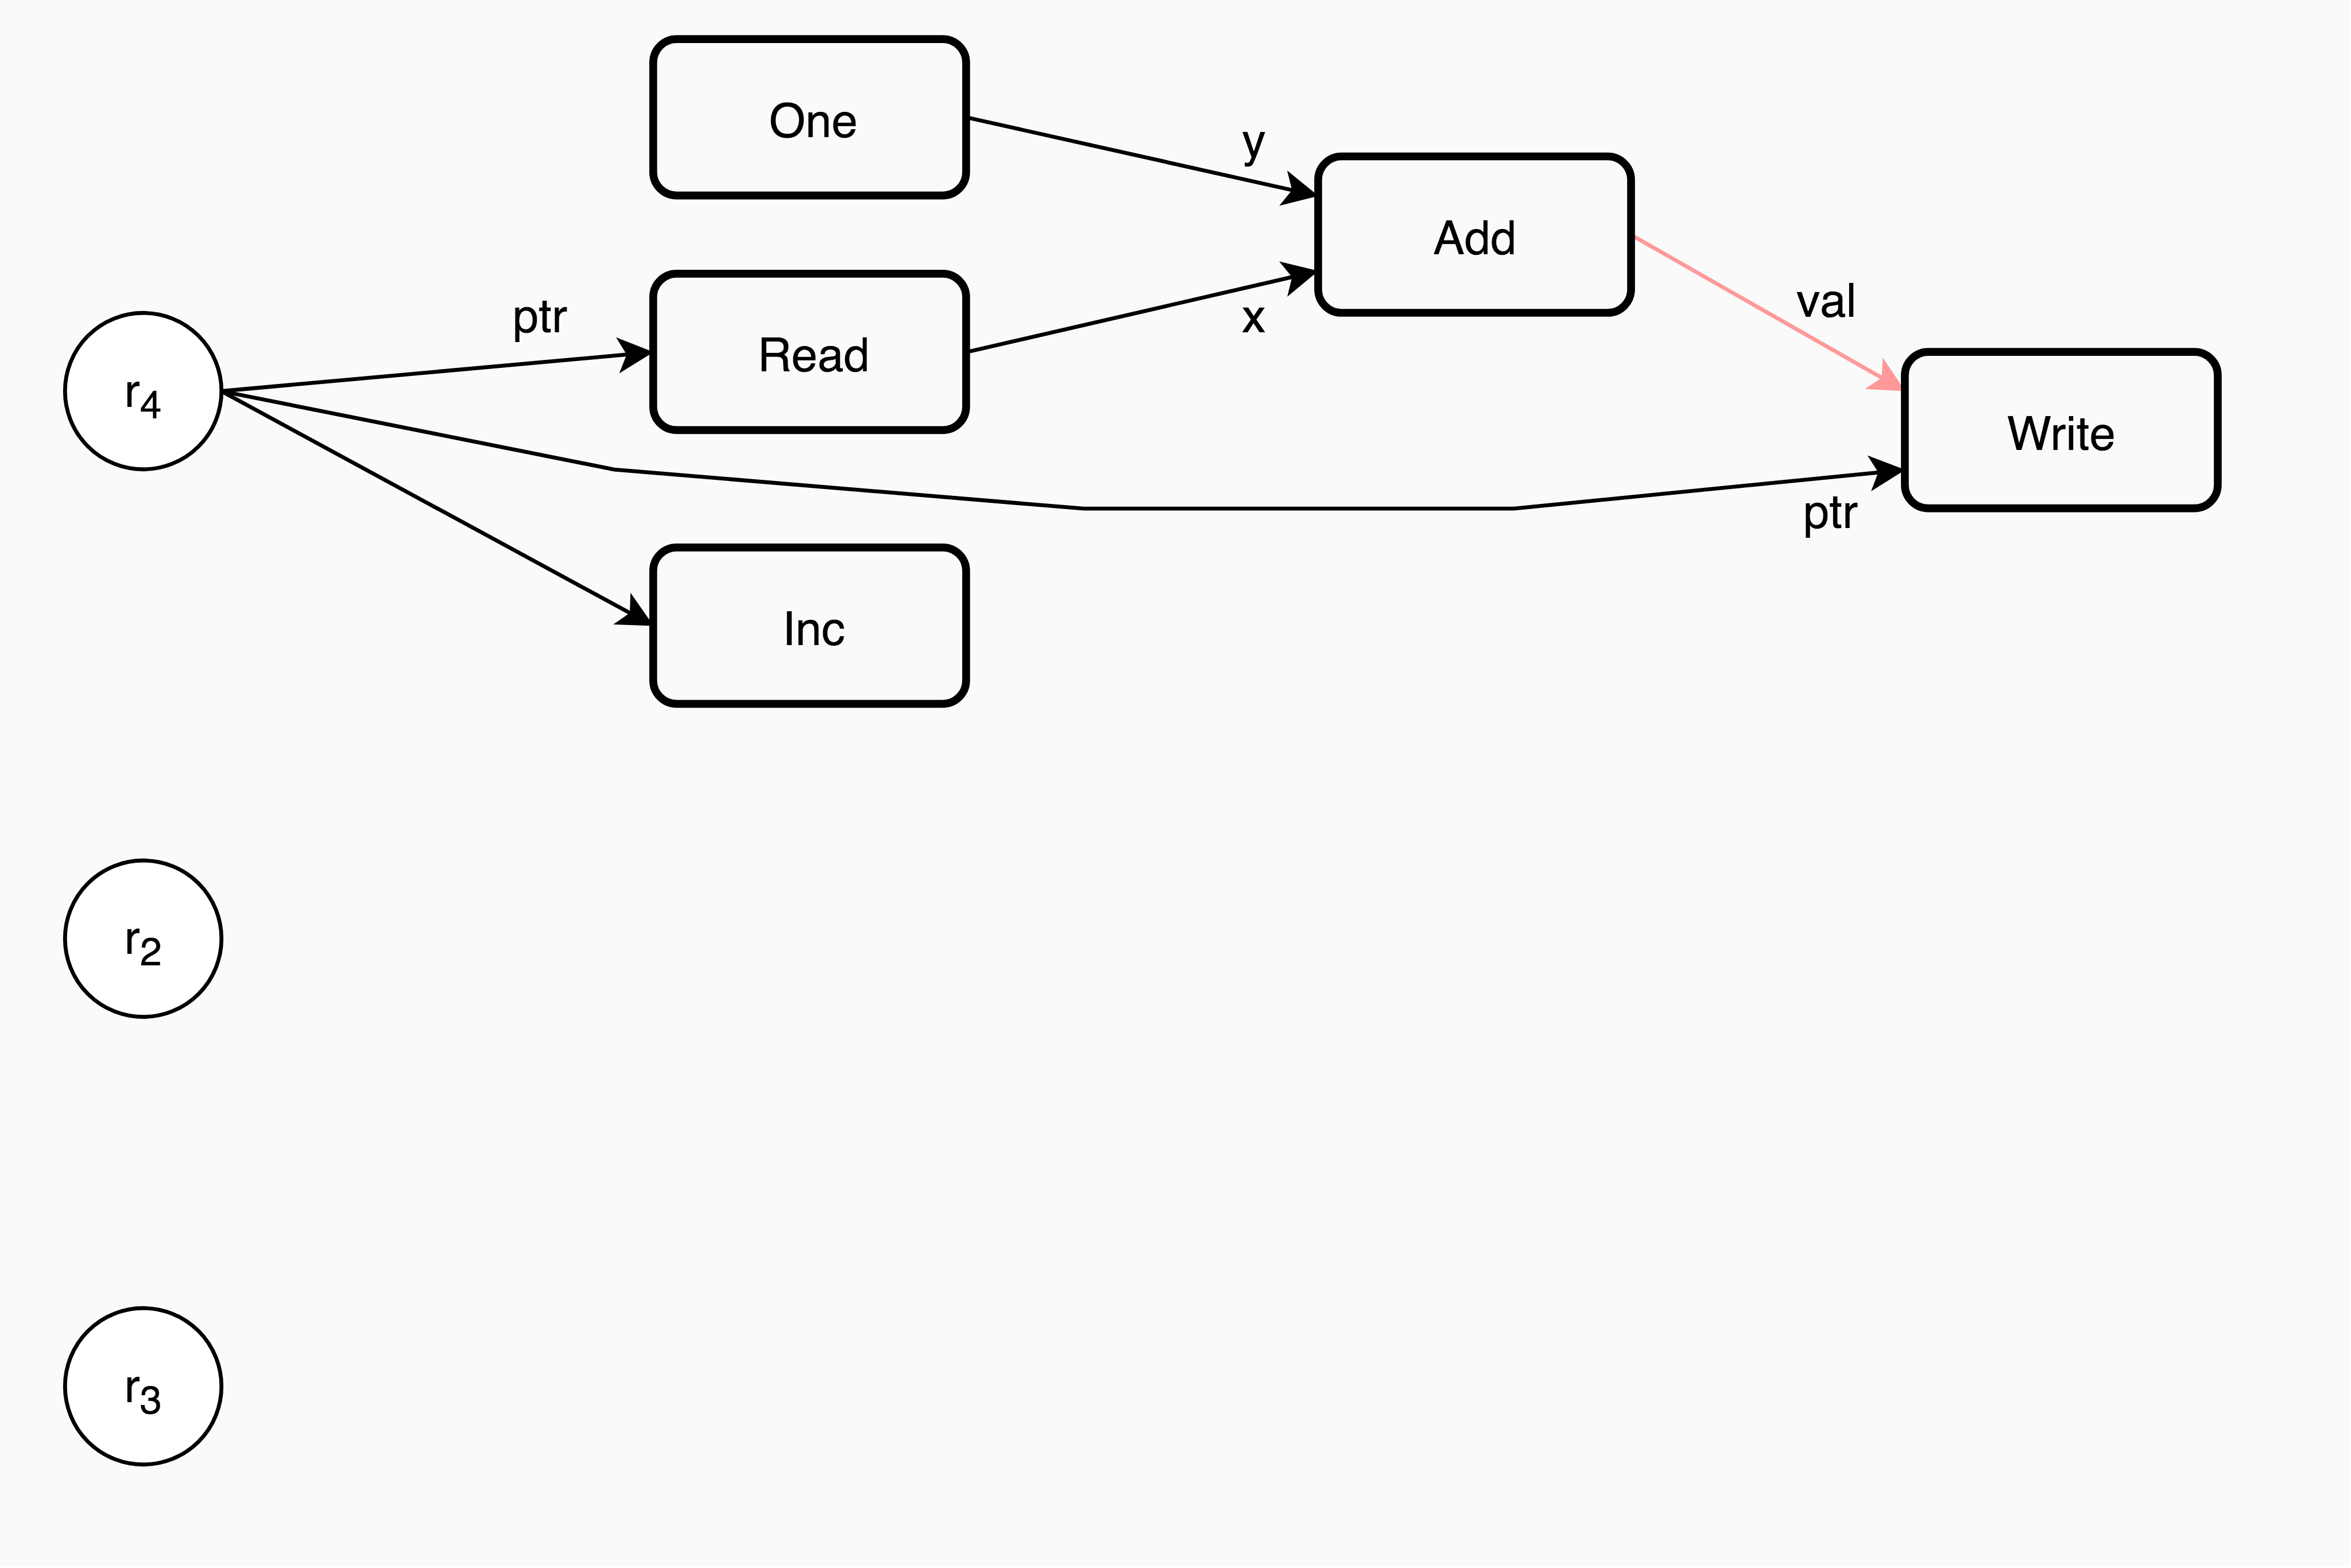
\includegraphics[width=\textwidth]{../figures/example-circuit-11.png}
  	\end{figure}
  \end{frame}
  \begin{frame}{Timestep execution - Circuit execution example}
  	\begin{figure}
  		\centering
  		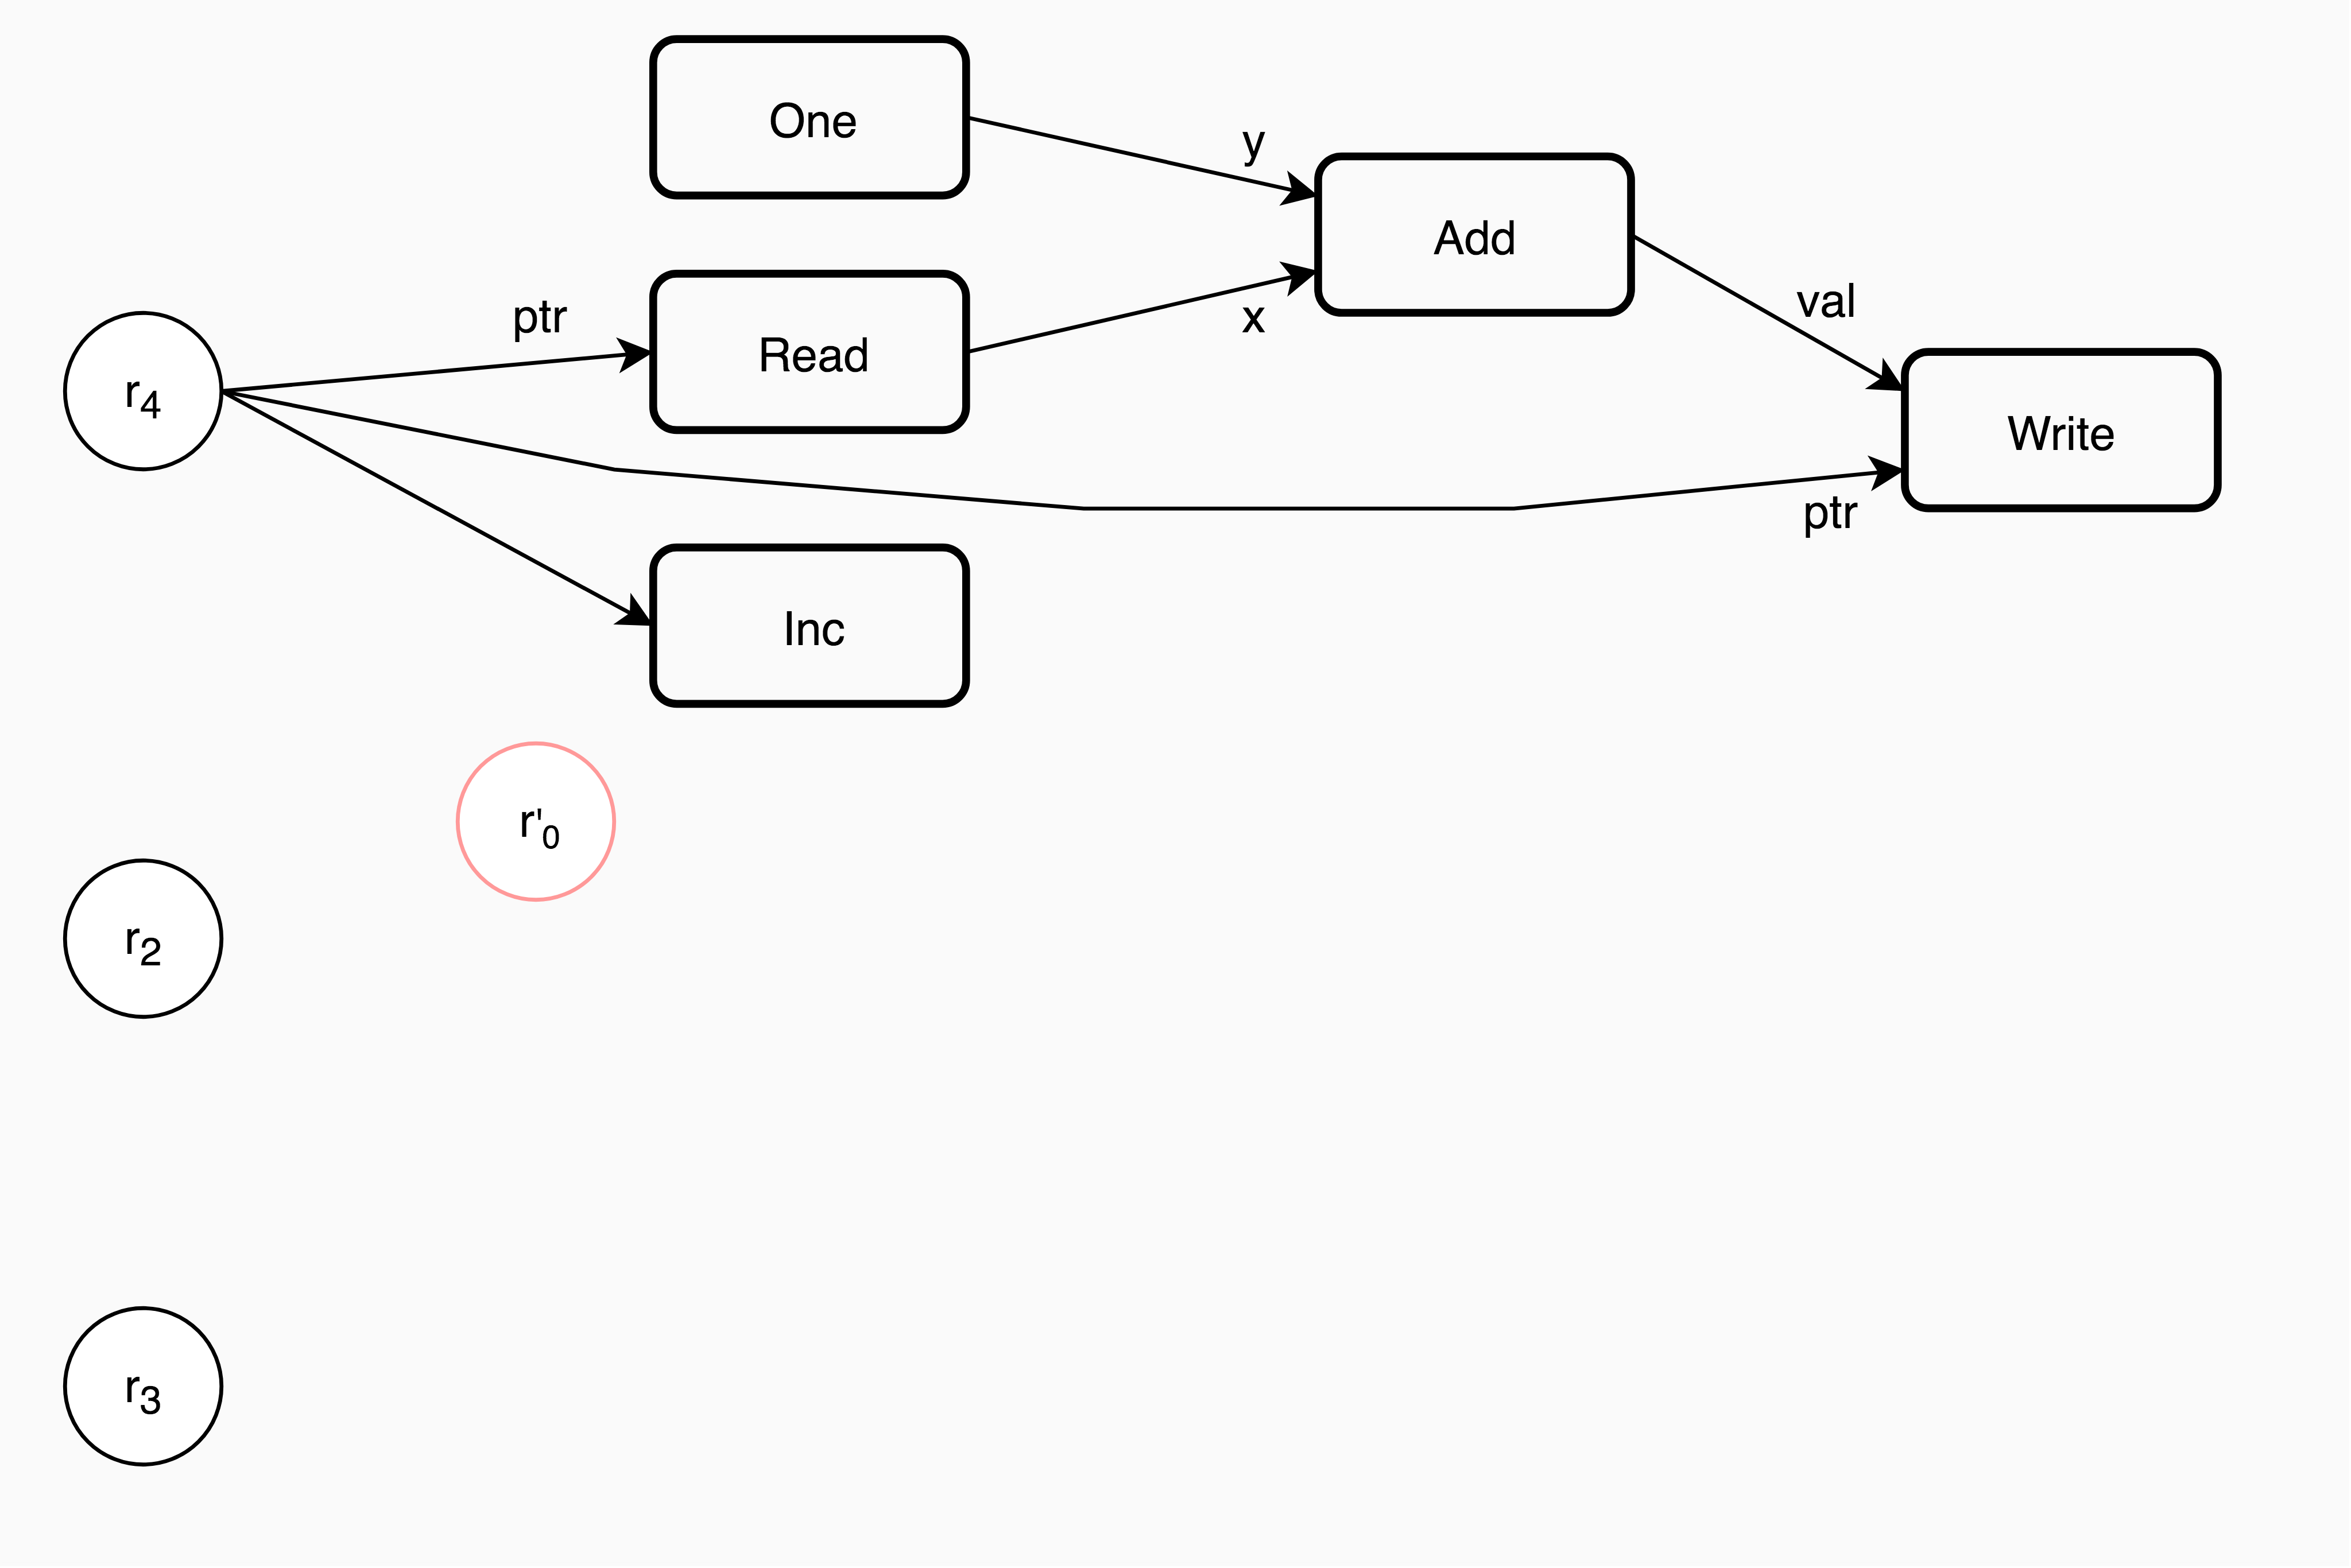
\includegraphics[width=\textwidth]{../figures/example-circuit-12.png}
  	\end{figure}
  \end{frame}
  \begin{frame}{Timestep execution - Circuit execution example}
  	\begin{figure}
  		\centering
  		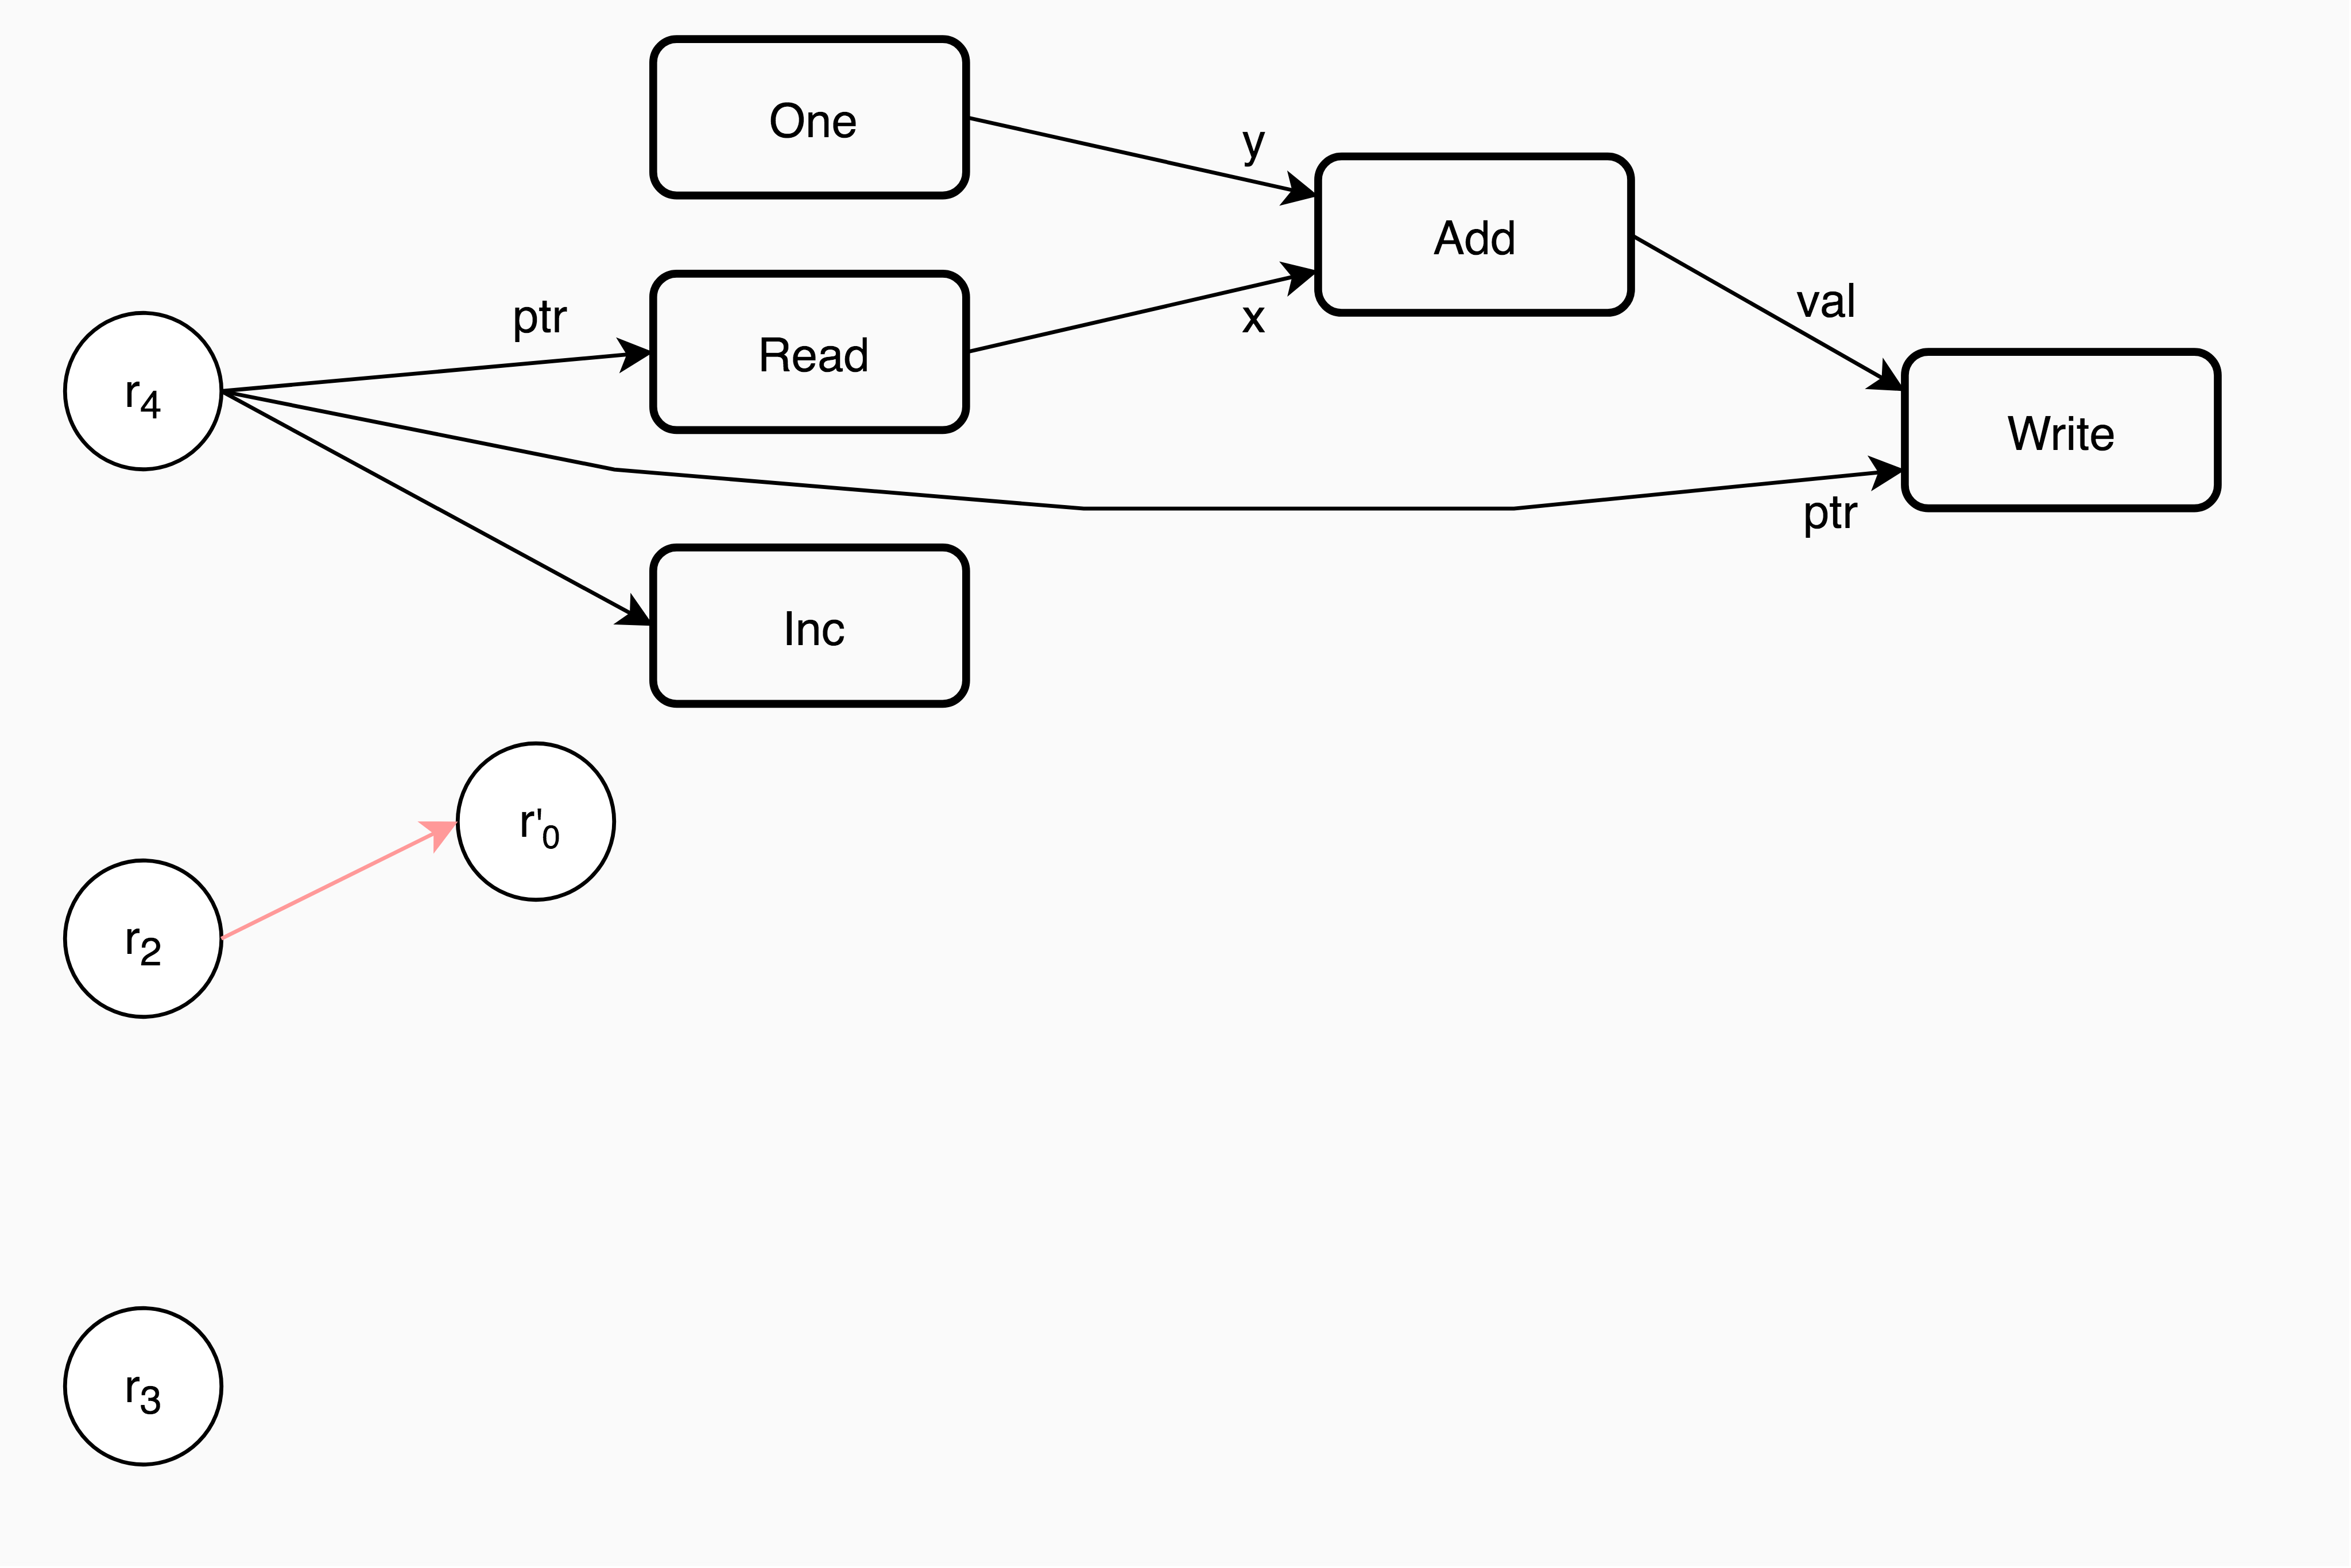
\includegraphics[width=\textwidth]{../figures/example-circuit-13.png}
  	\end{figure}
  \end{frame}
  \begin{frame}{Timestep execution - Circuit execution example}
  	\begin{figure}
  		\centering
  		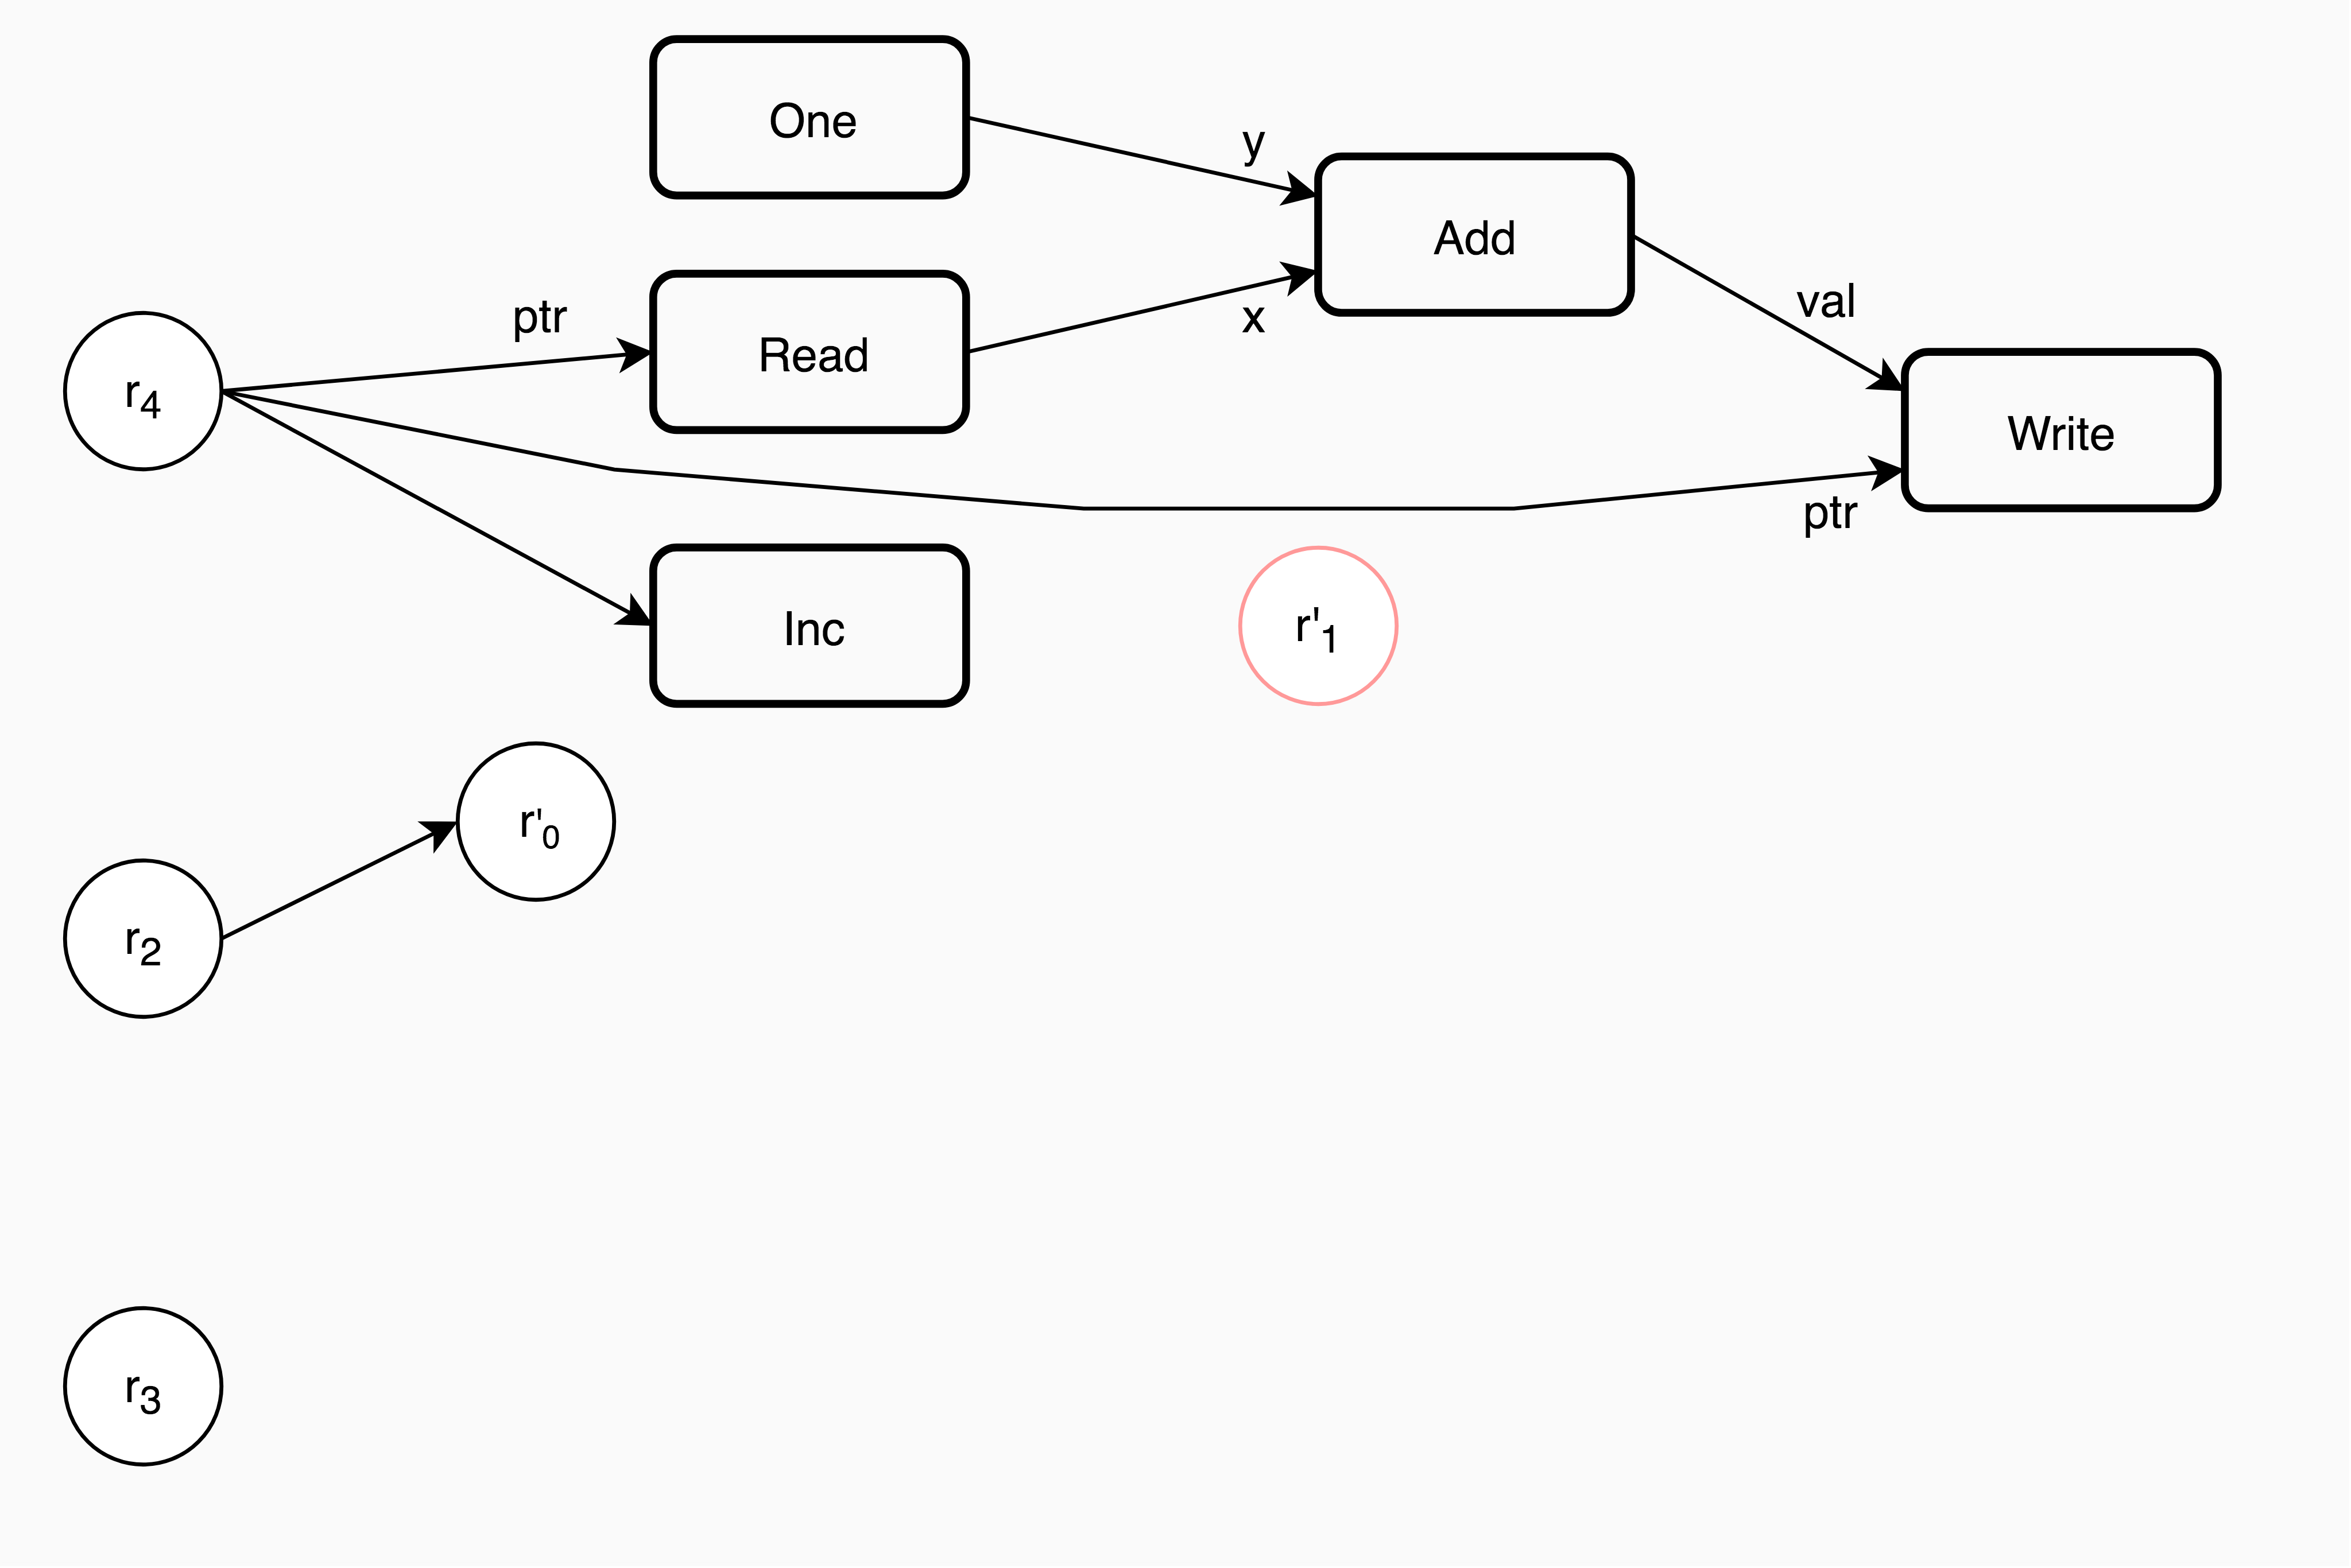
\includegraphics[width=\textwidth]{../figures/example-circuit-14.png}
  	\end{figure}
  \end{frame}
  \begin{frame}{Timestep execution - Circuit execution example}
  	\begin{figure}
  		\centering
  		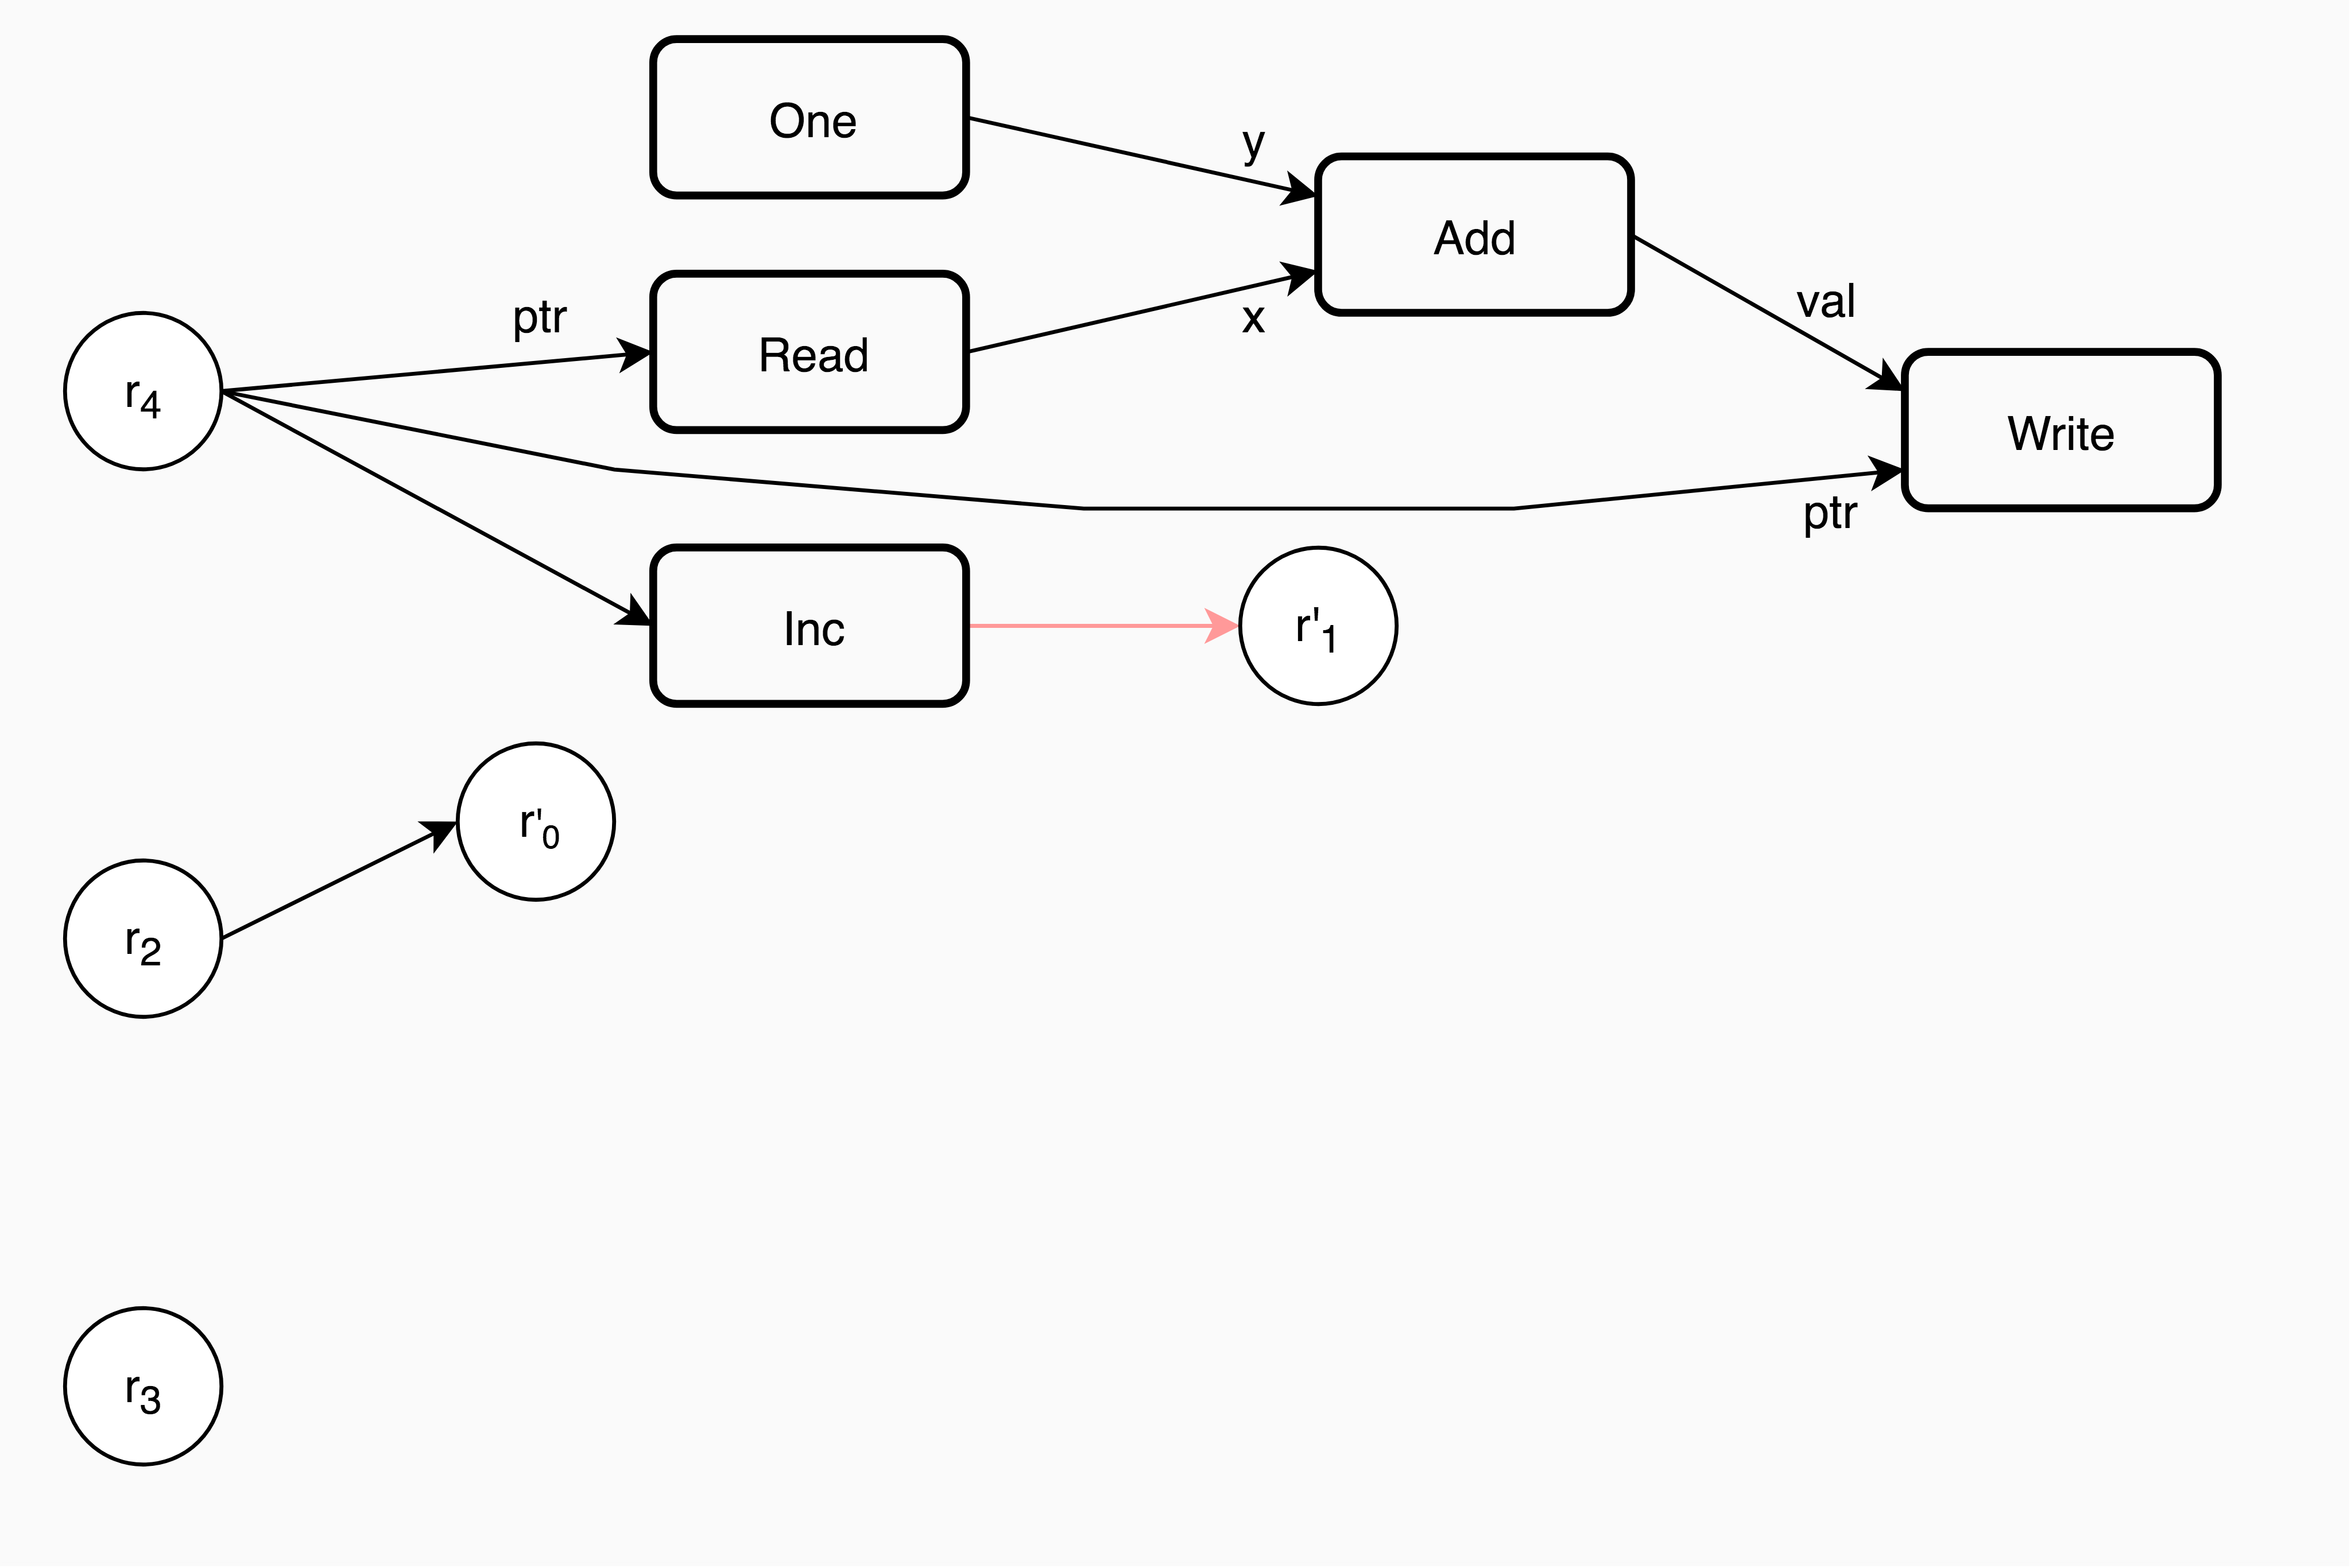
\includegraphics[width=\textwidth]{../figures/example-circuit-15.png}
  	\end{figure}
  \end{frame}
  \begin{frame}{Timestep execution - Circuit execution example}
  	\begin{figure}
  		\centering
  		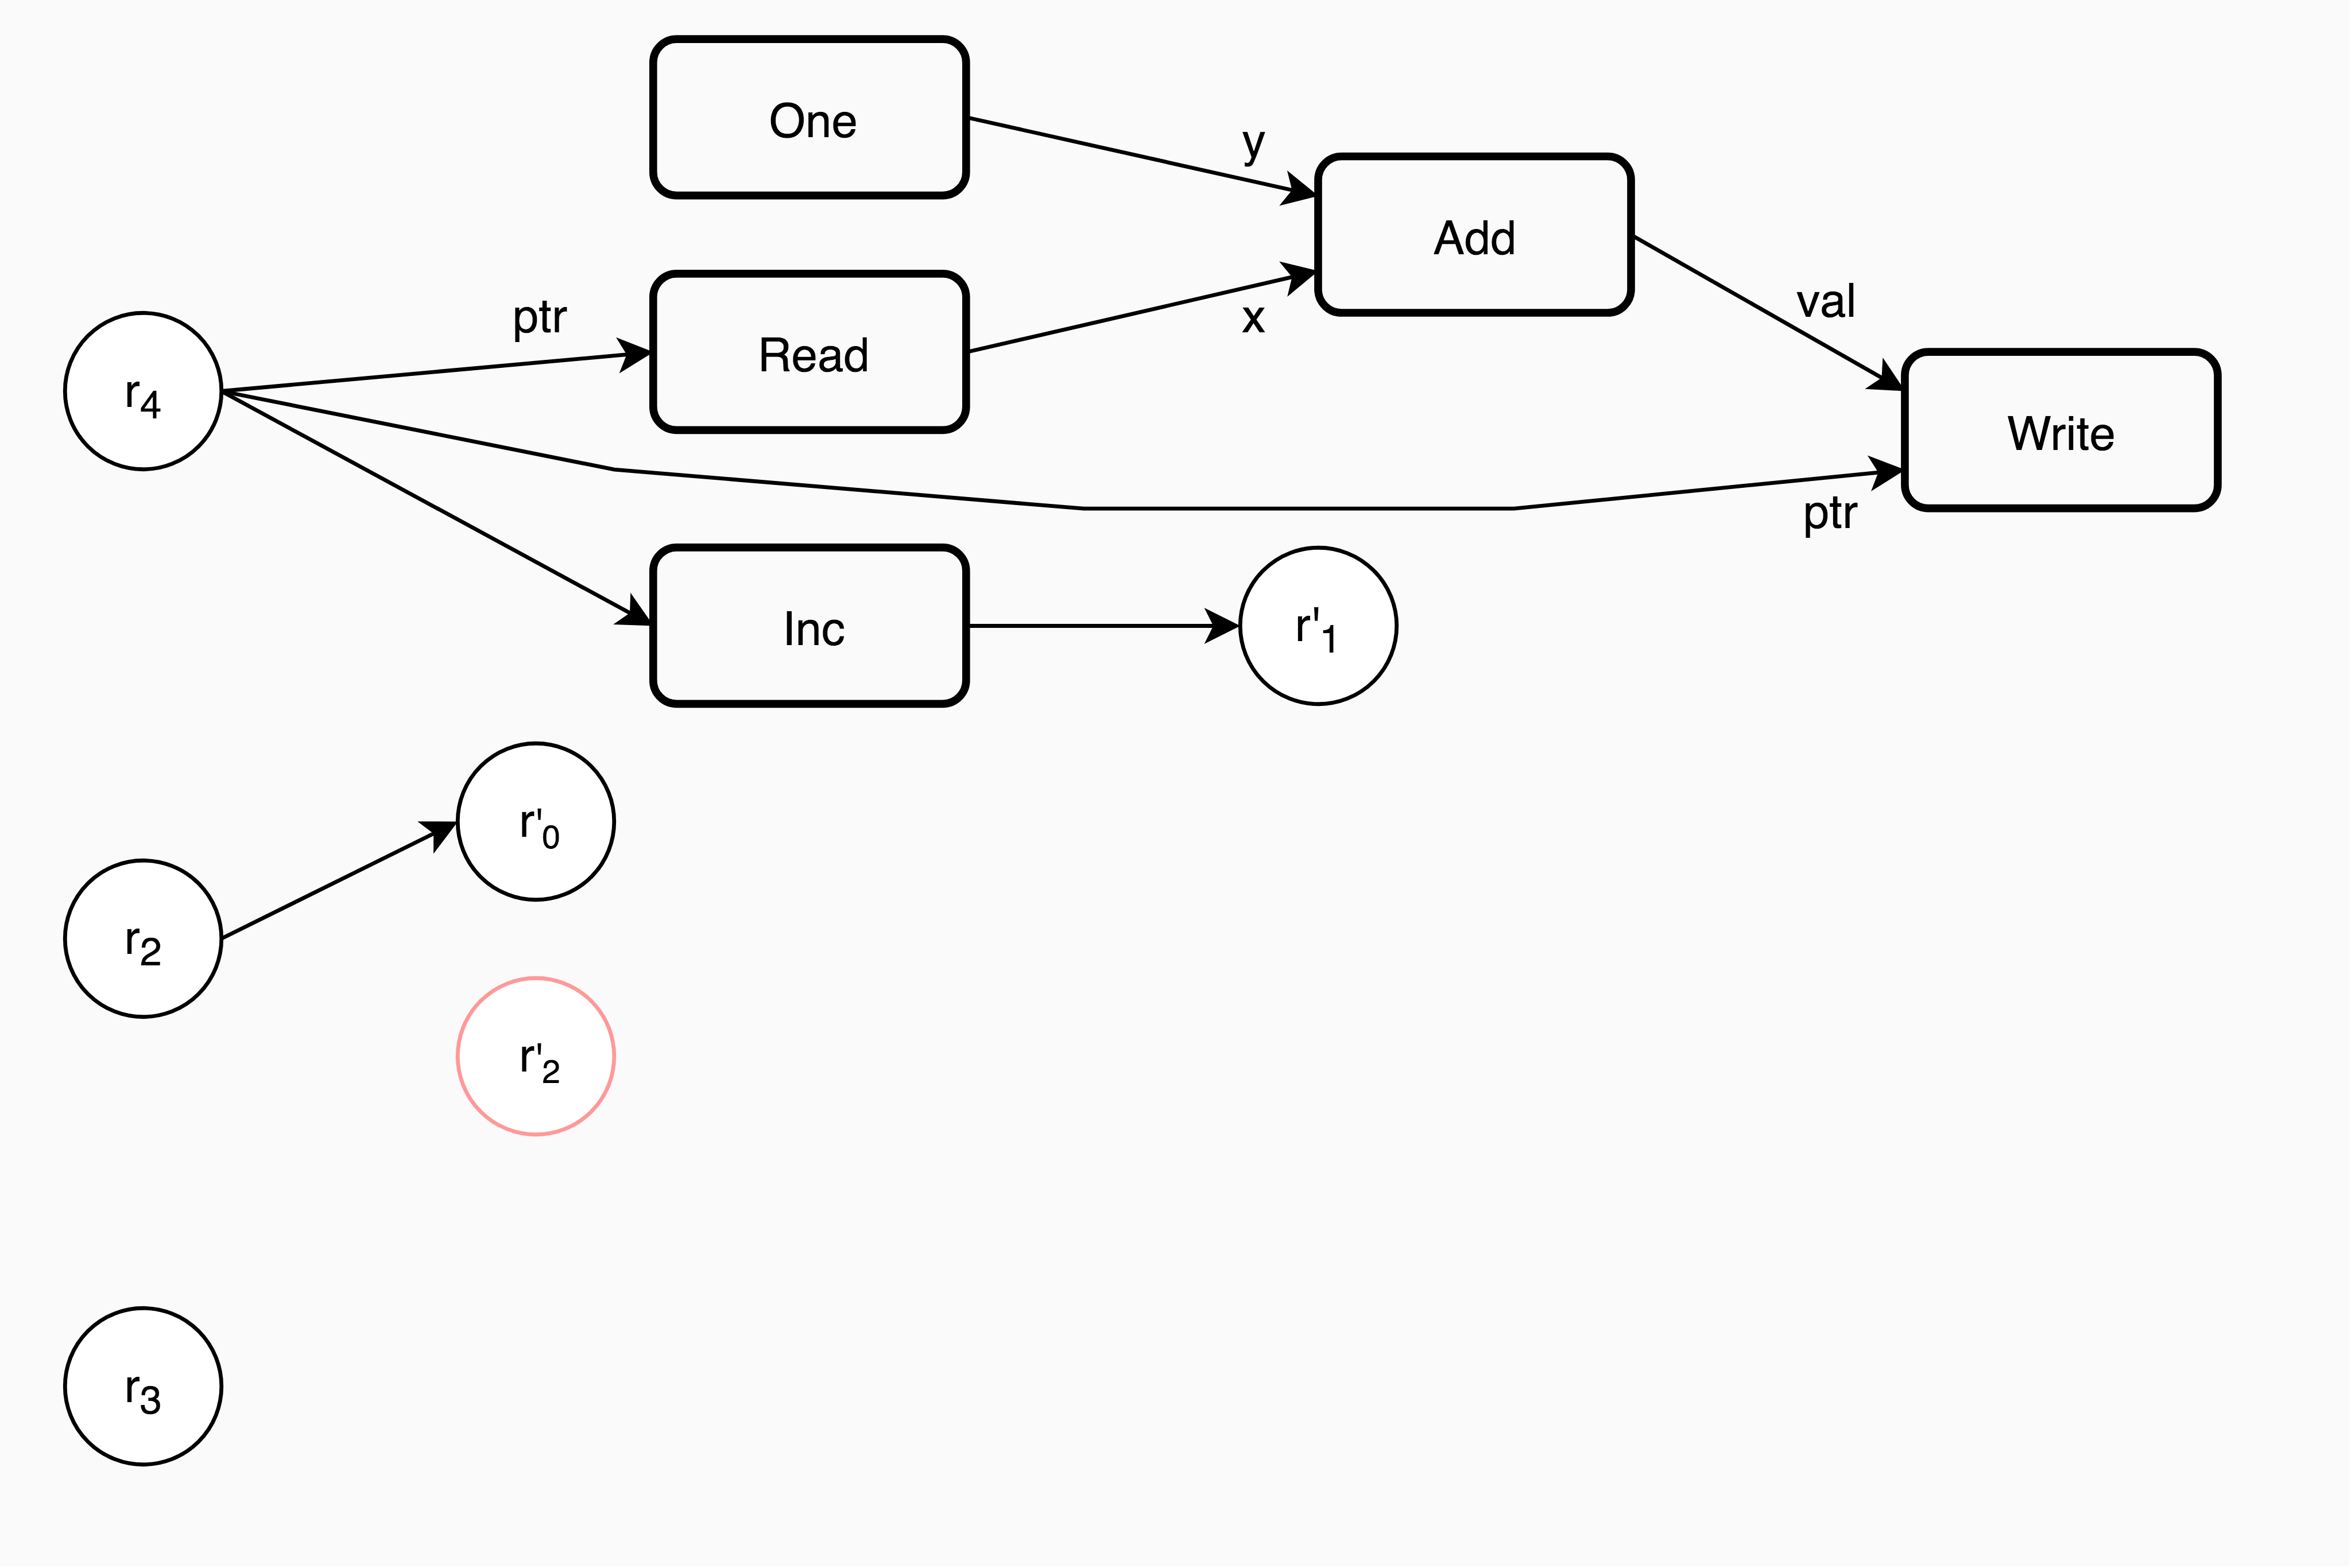
\includegraphics[width=\textwidth]{../figures/example-circuit-16.png}
  	\end{figure}
  \end{frame}
  \begin{frame}{Timestep execution - Circuit execution example}
  	\begin{figure}
  		\centering
  		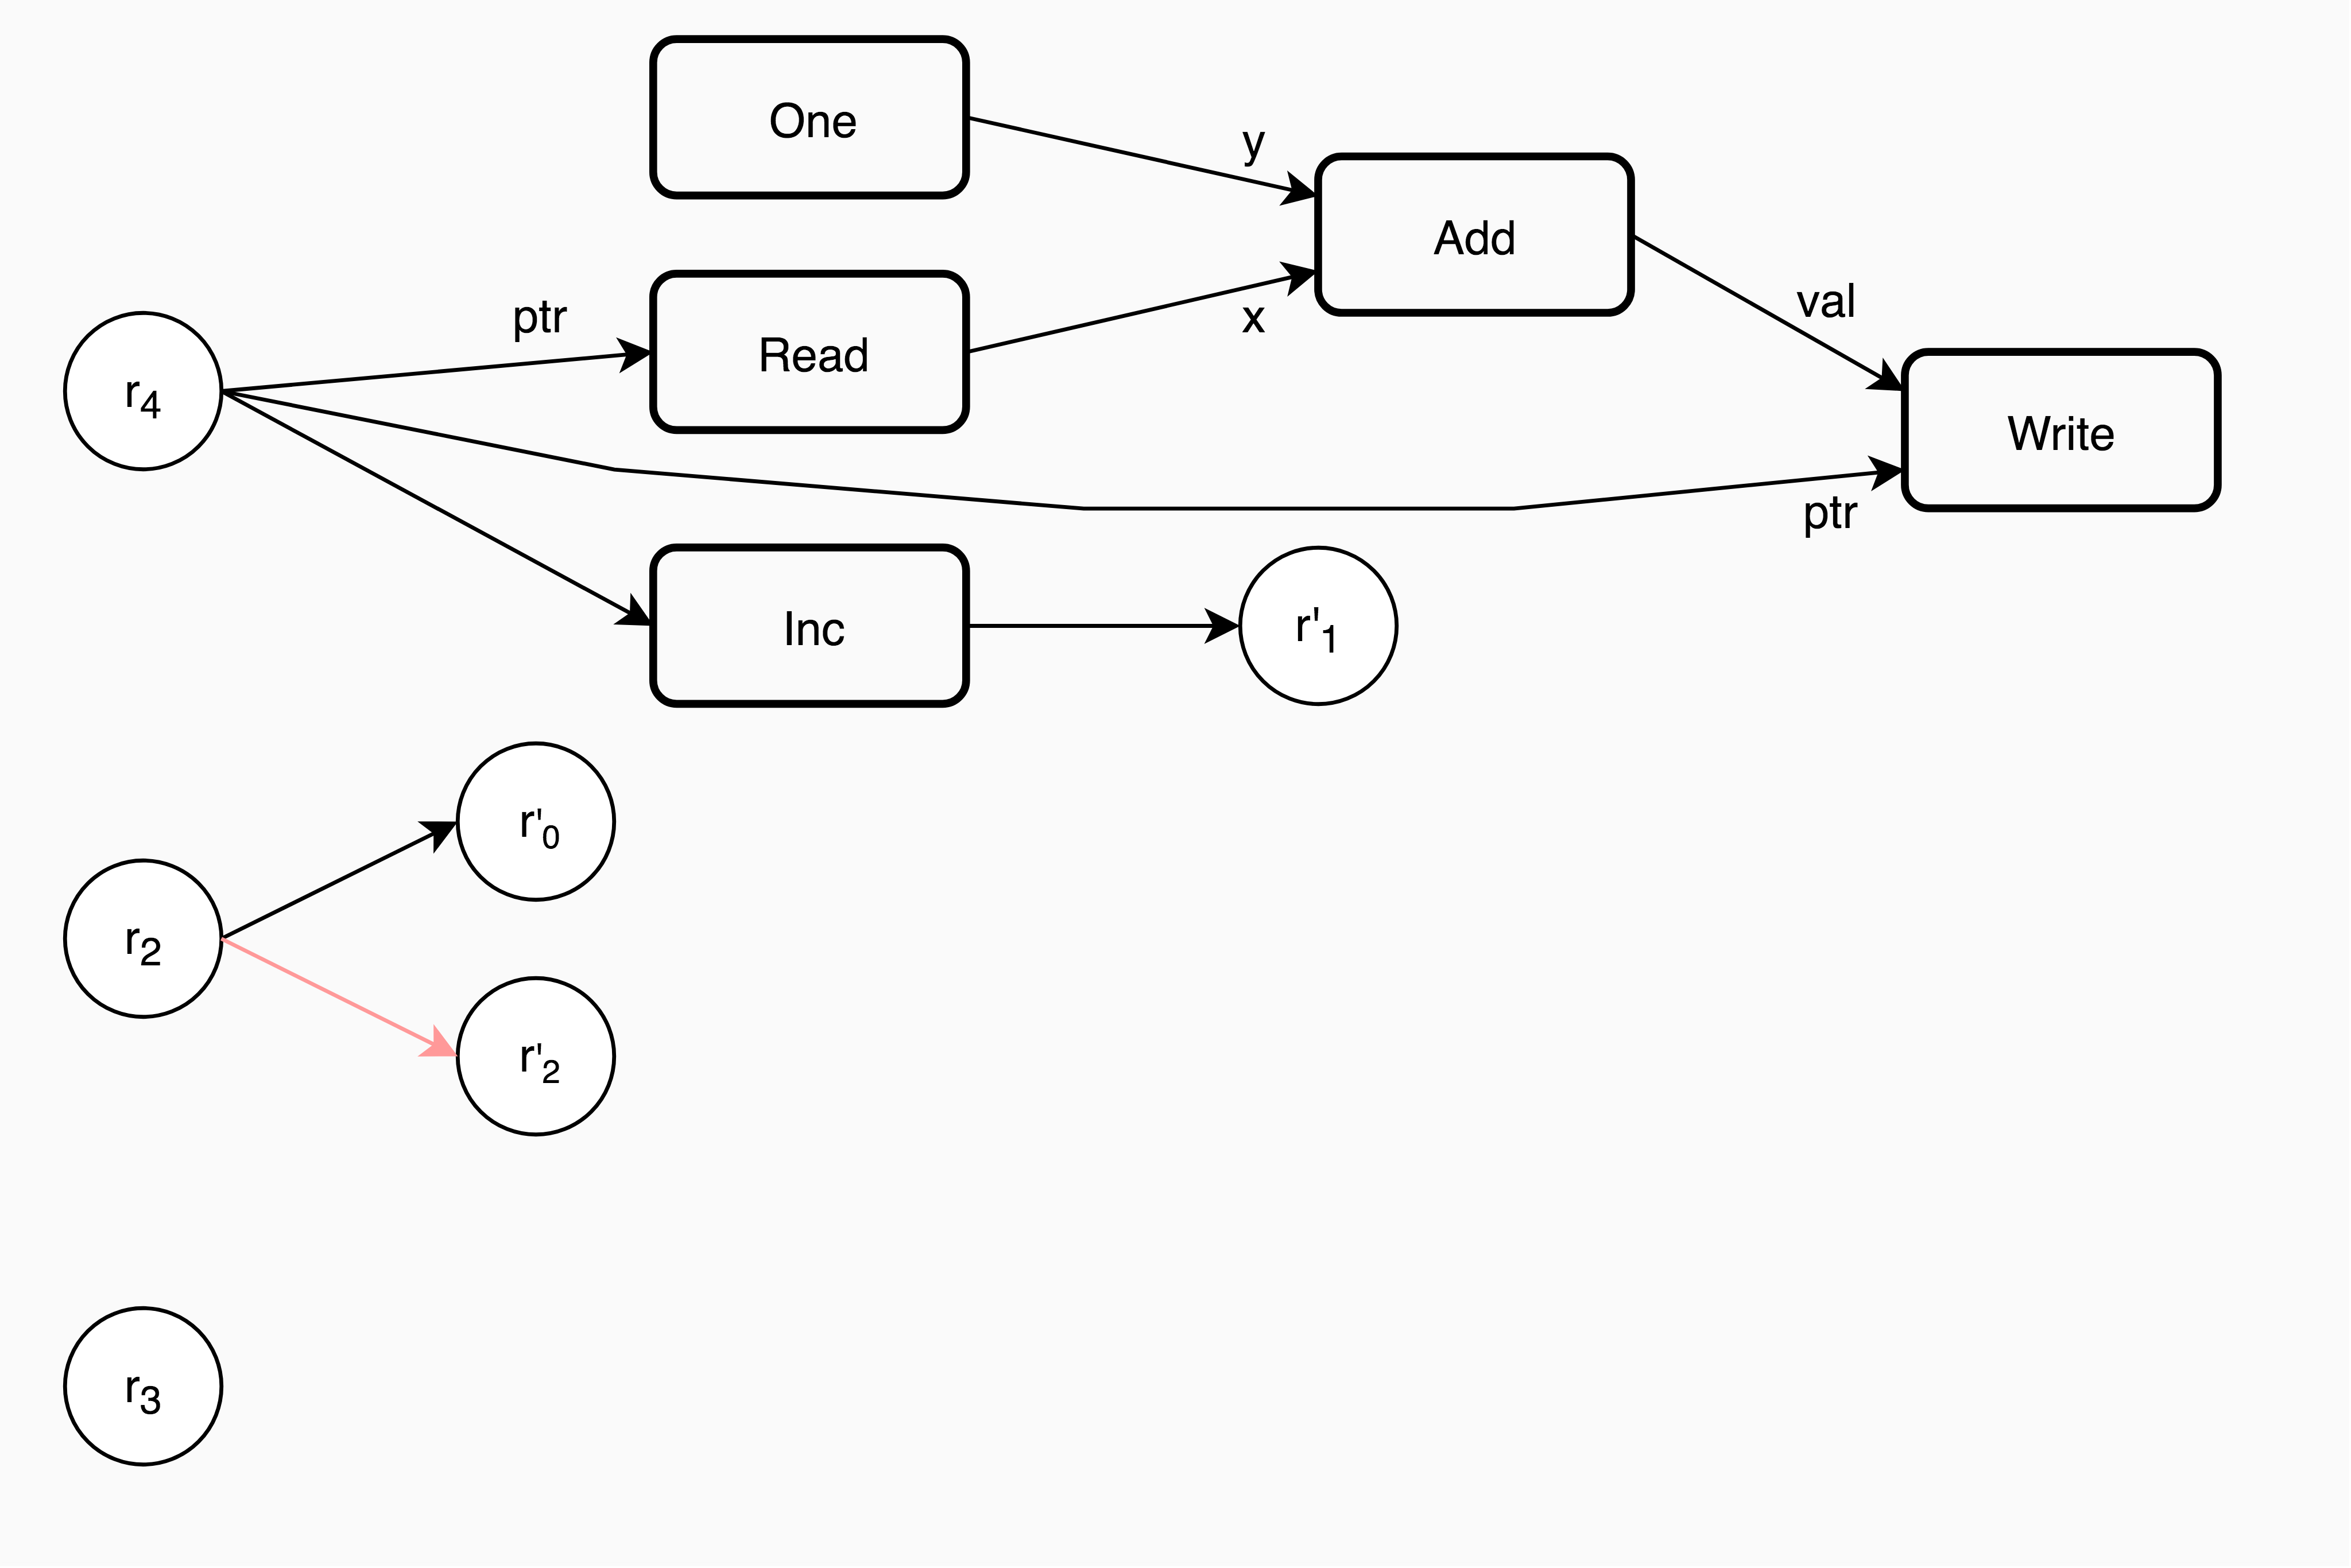
\includegraphics[width=\textwidth]{../figures/example-circuit-17.png}
  	\end{figure}
  \end{frame}
  \begin{frame}{Timestep execution - Circuit execution example}
  	\begin{figure}
  		\centering
  		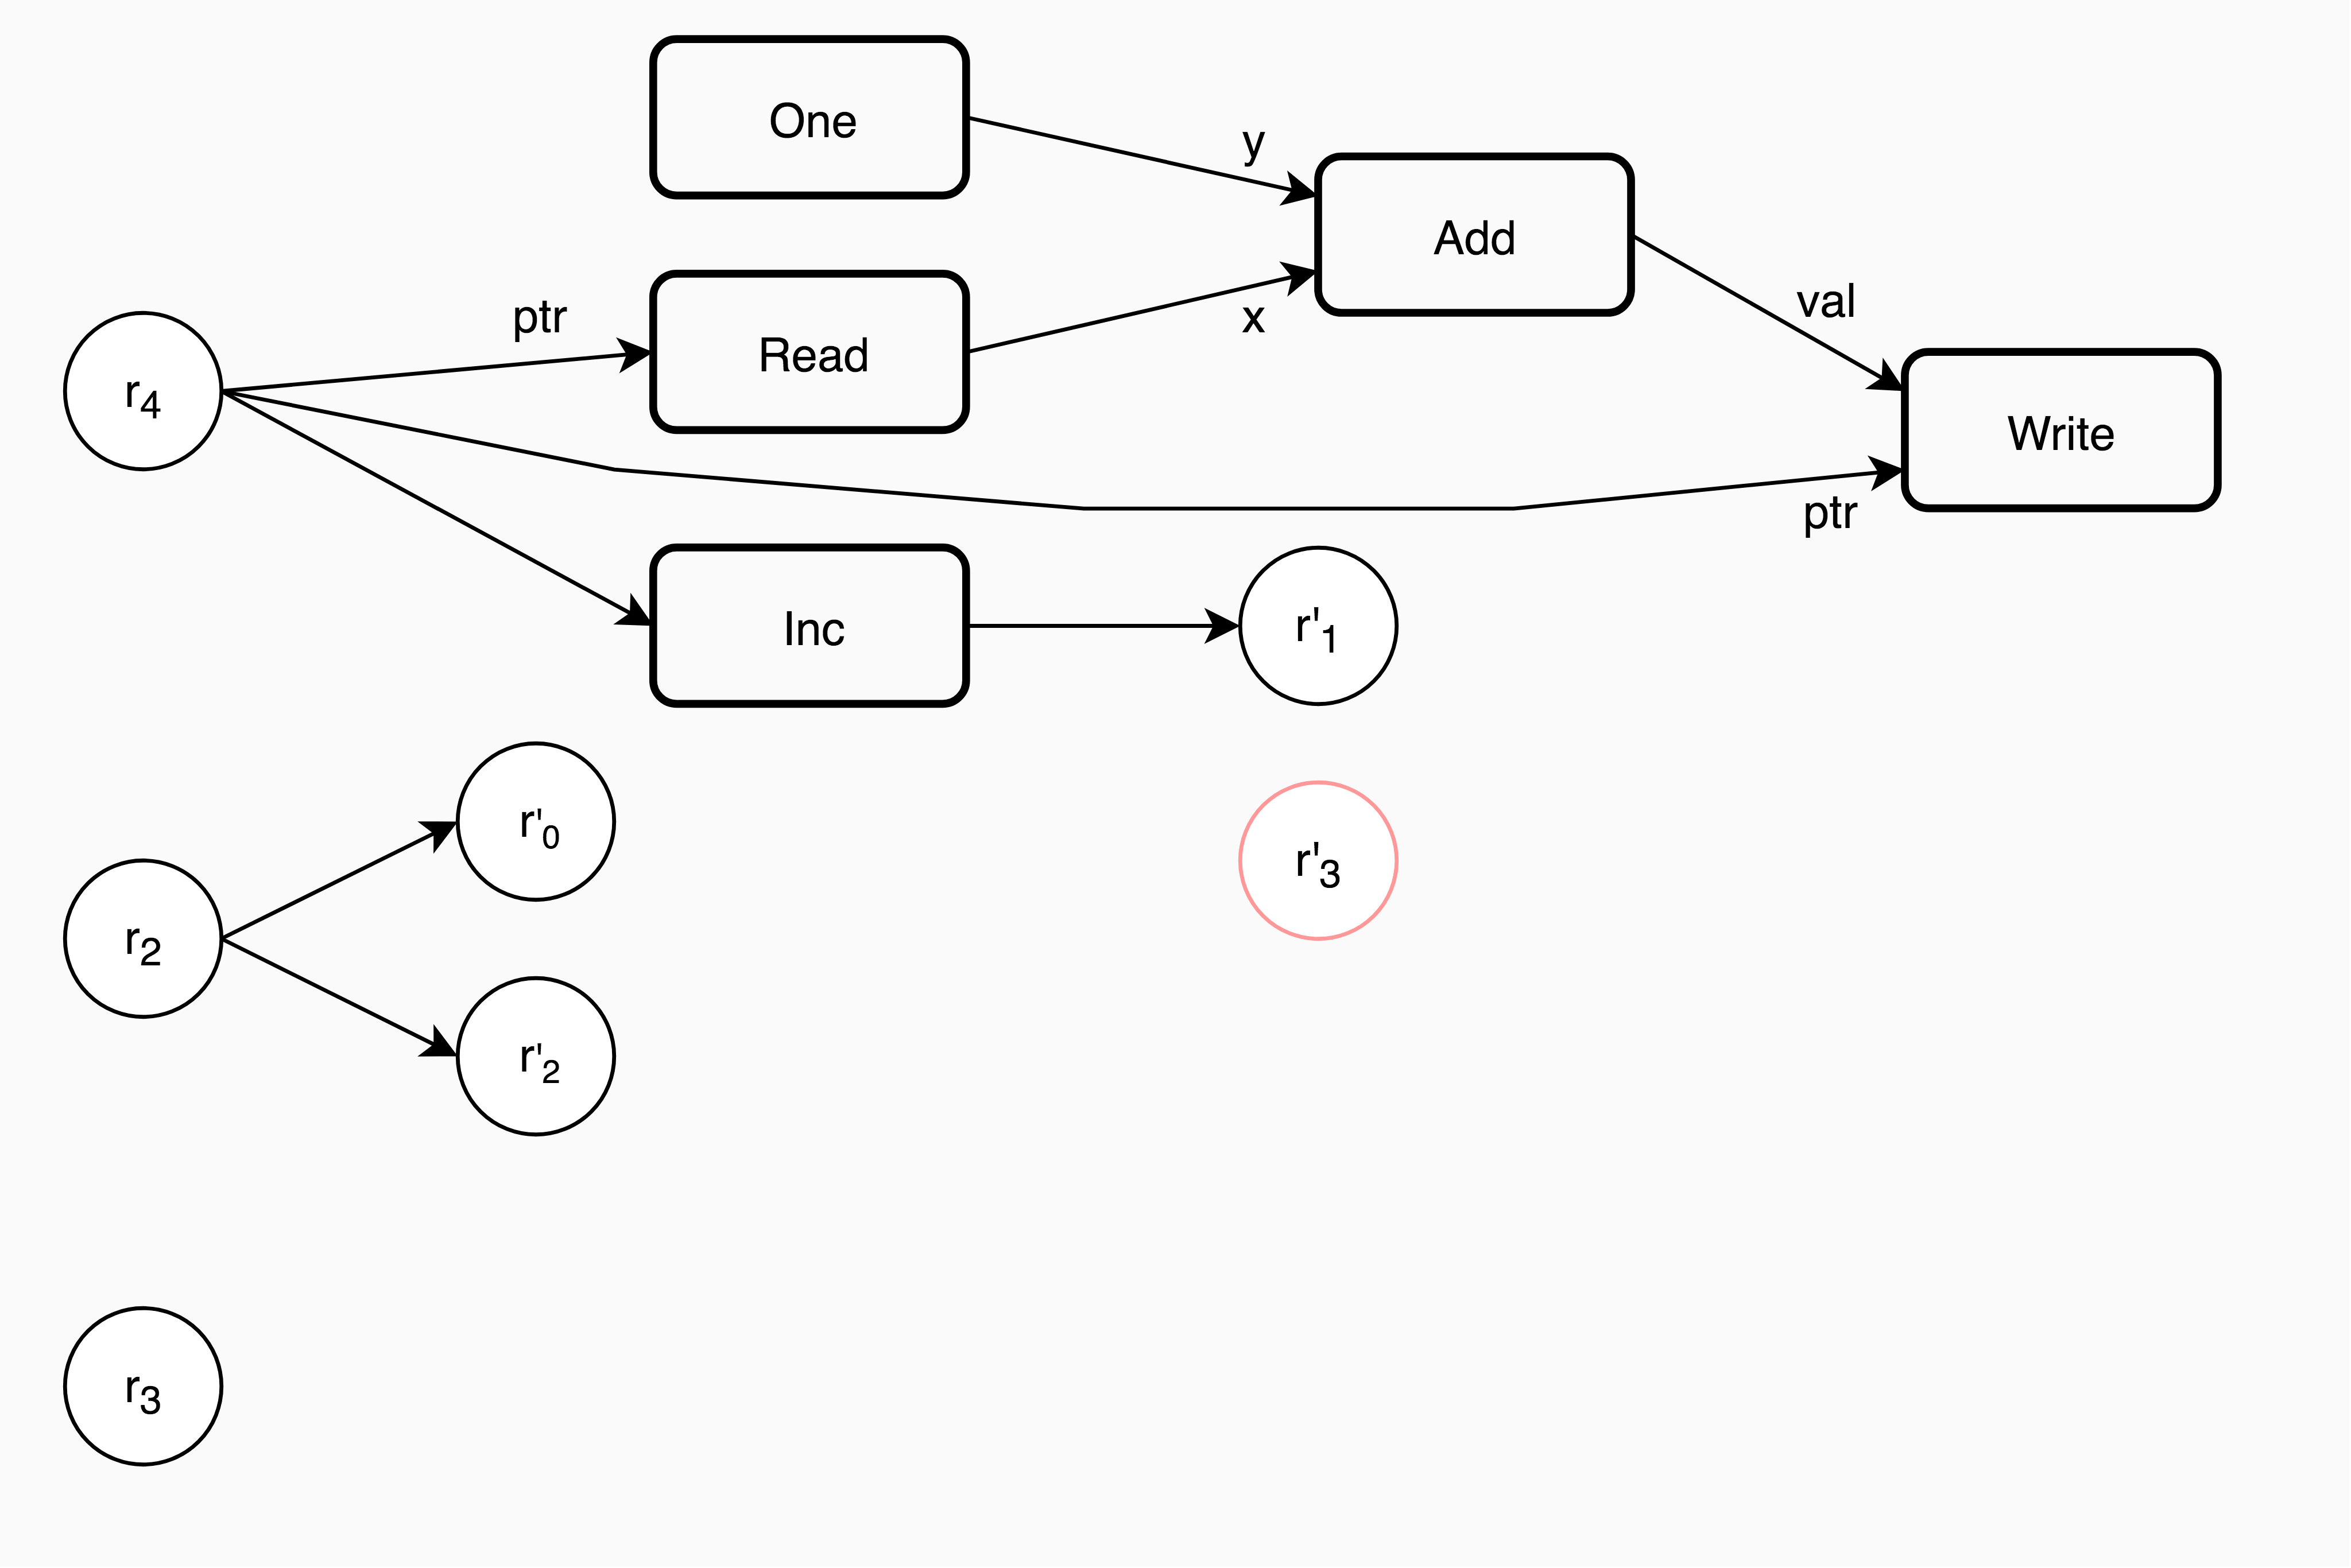
\includegraphics[width=\textwidth]{../figures/example-circuit-18.png}
  	\end{figure}
  \end{frame}
  \begin{frame}{Timestep execution - Circuit execution example}
  	\begin{figure}
  		\centering
  		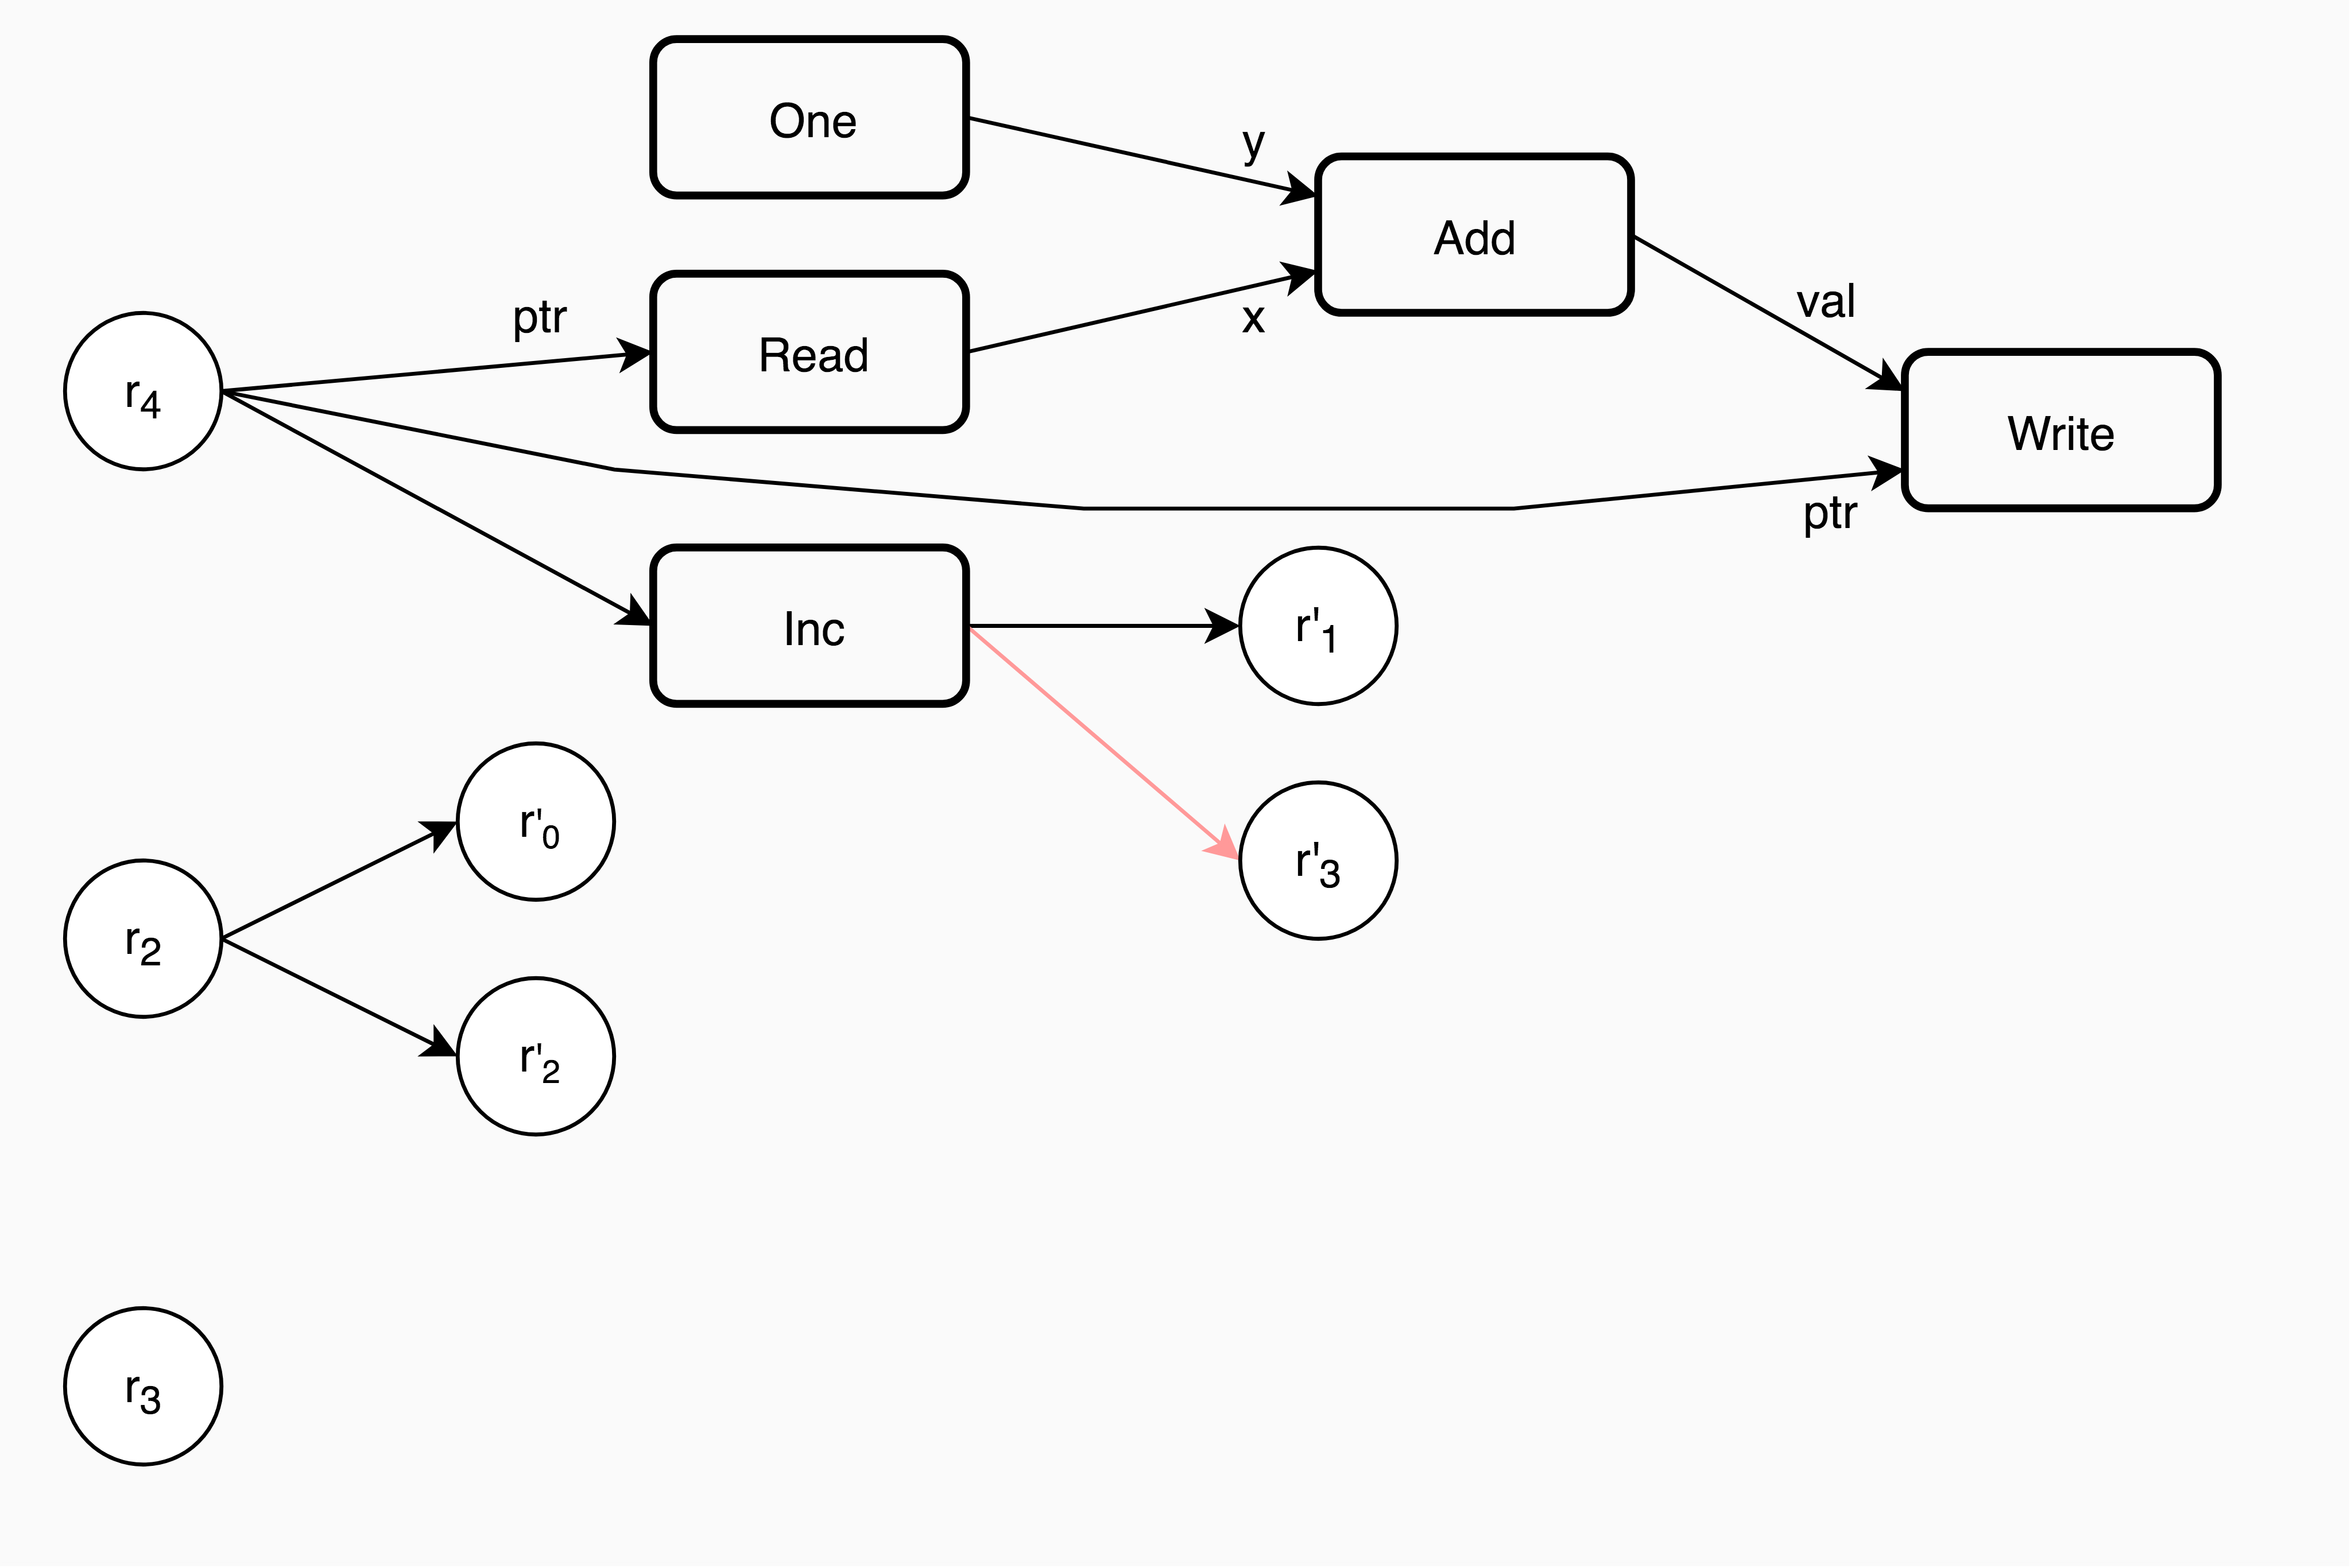
\includegraphics[width=\textwidth]{../figures/example-circuit-19.png}
  	\end{figure}
  \end{frame}
  \begin{frame}{Timestep execution - Circuit execution example}
  	\begin{figure}
  		\centering
  		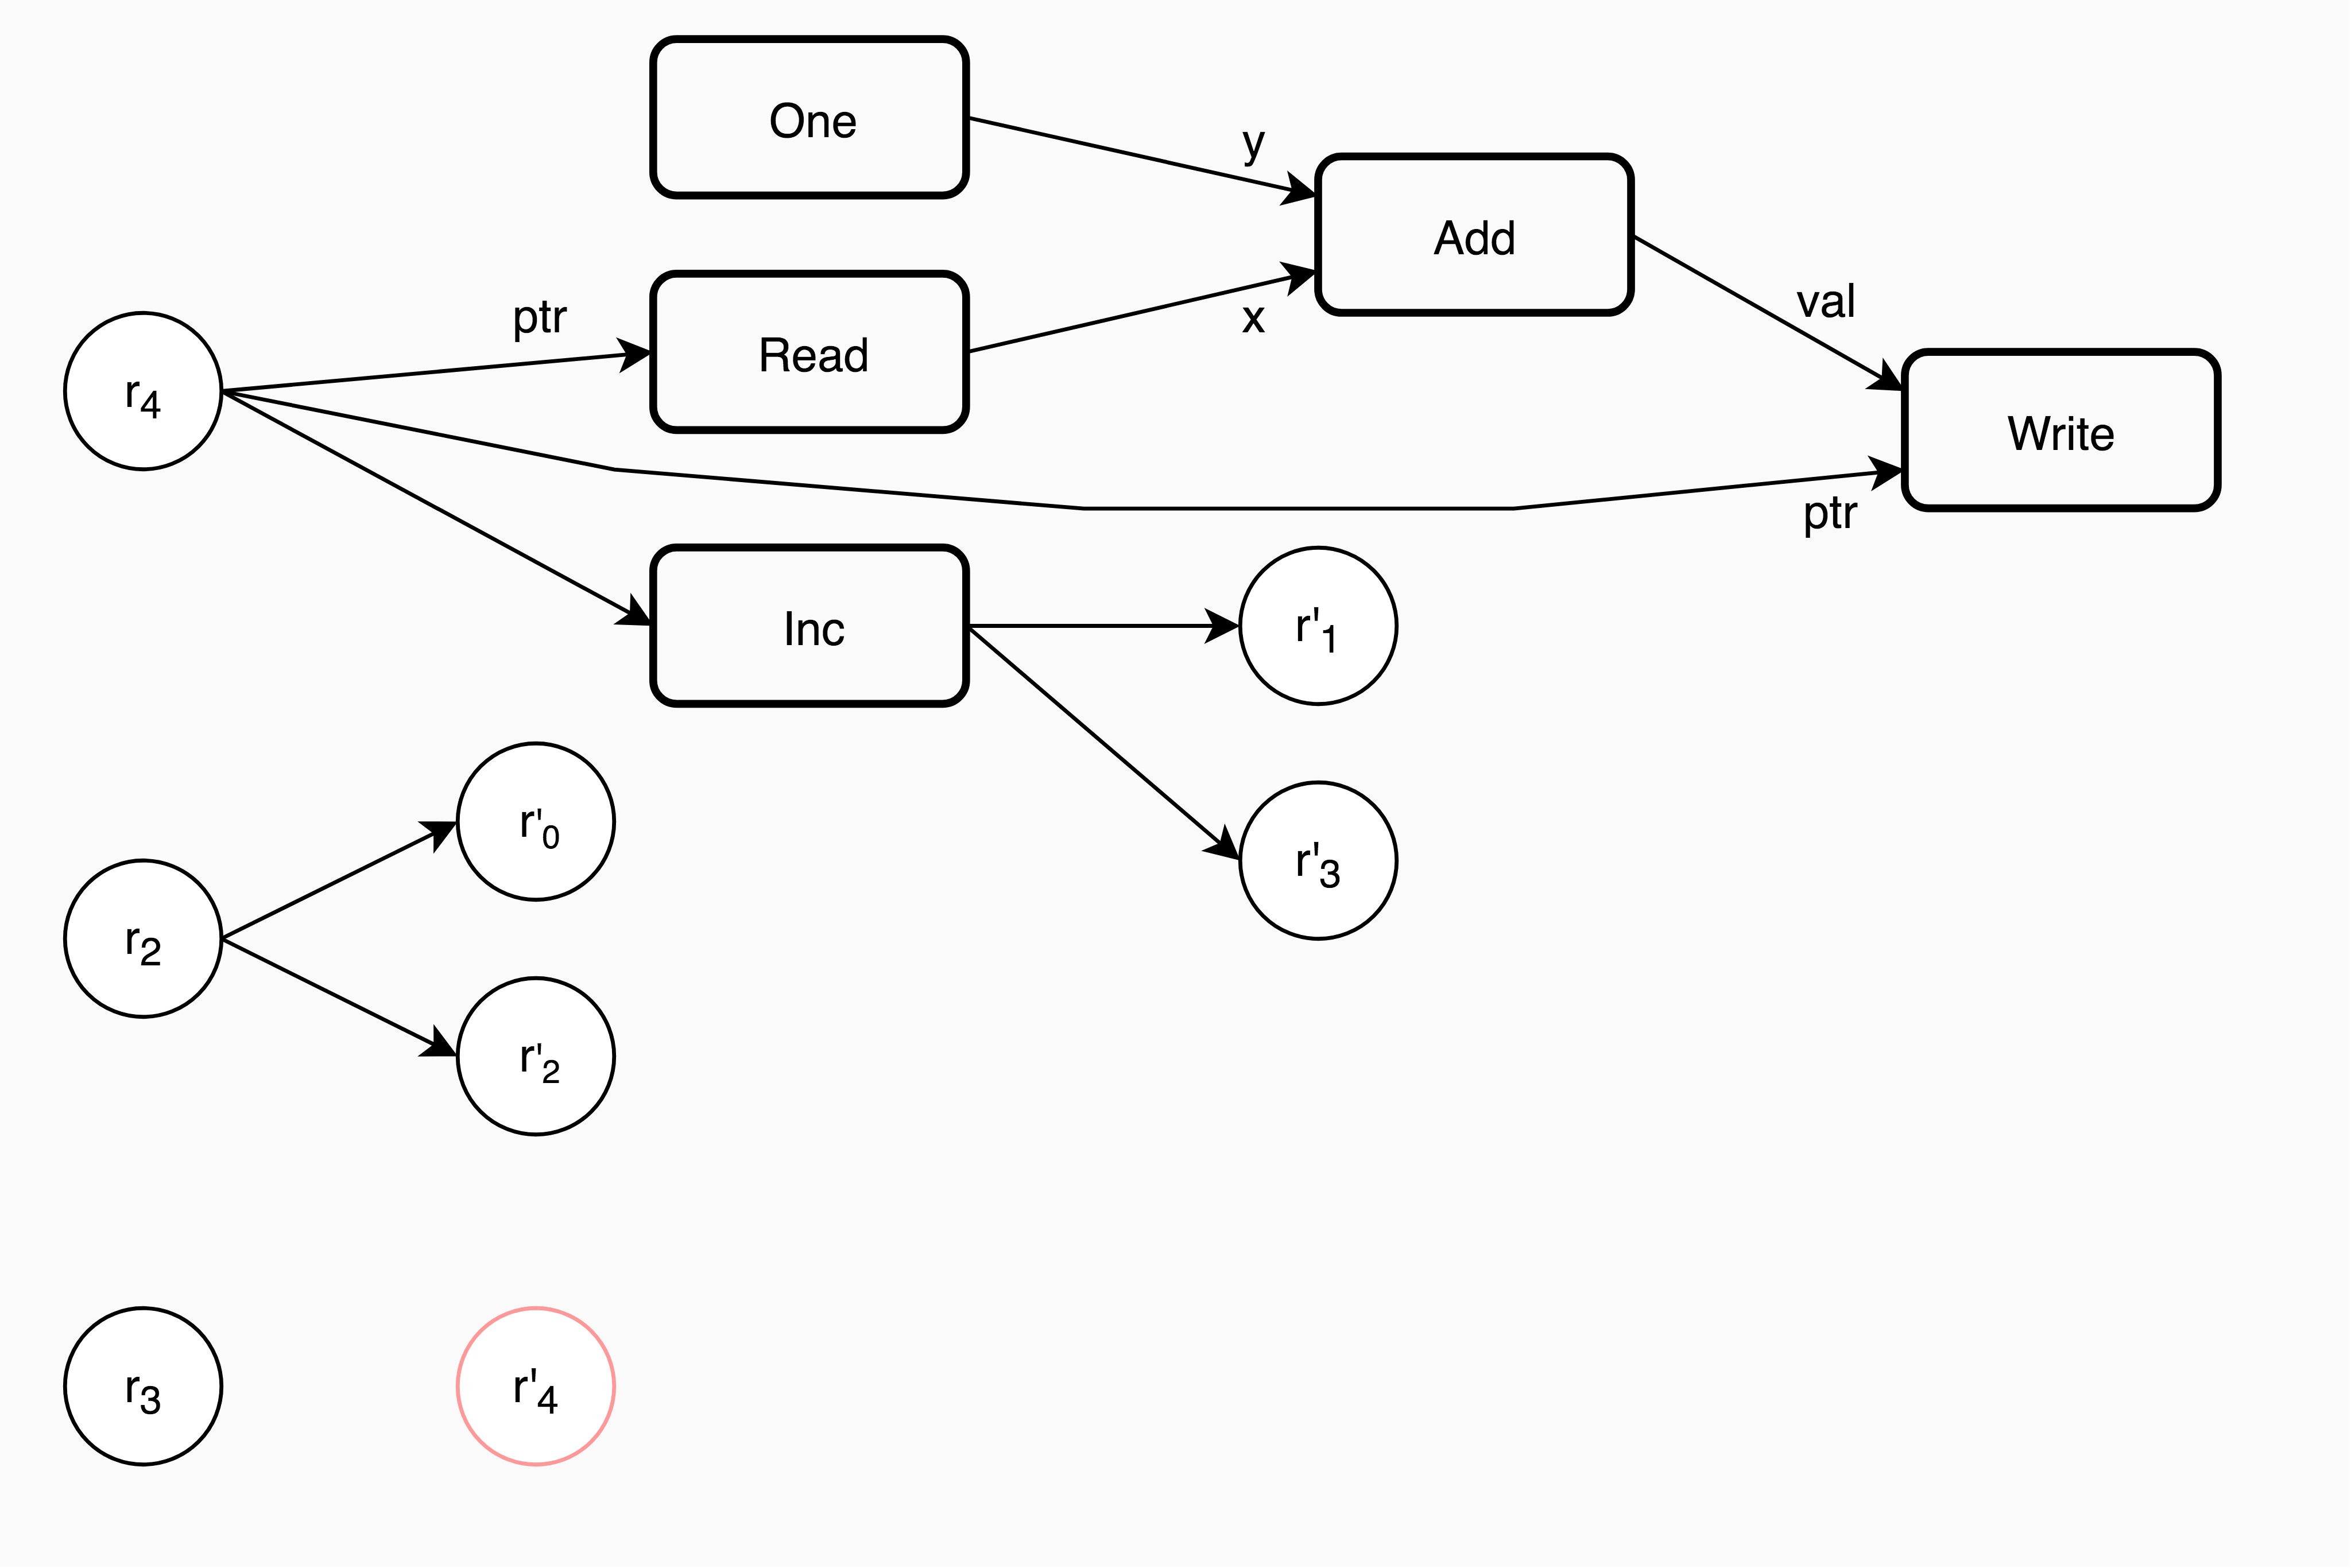
\includegraphics[width=\textwidth]{../figures/example-circuit-20.png}
  	\end{figure}
  \end{frame}
  \begin{frame}{Timestep execution - Circuit execution example}
  	\begin{figure}
  		\centering
  		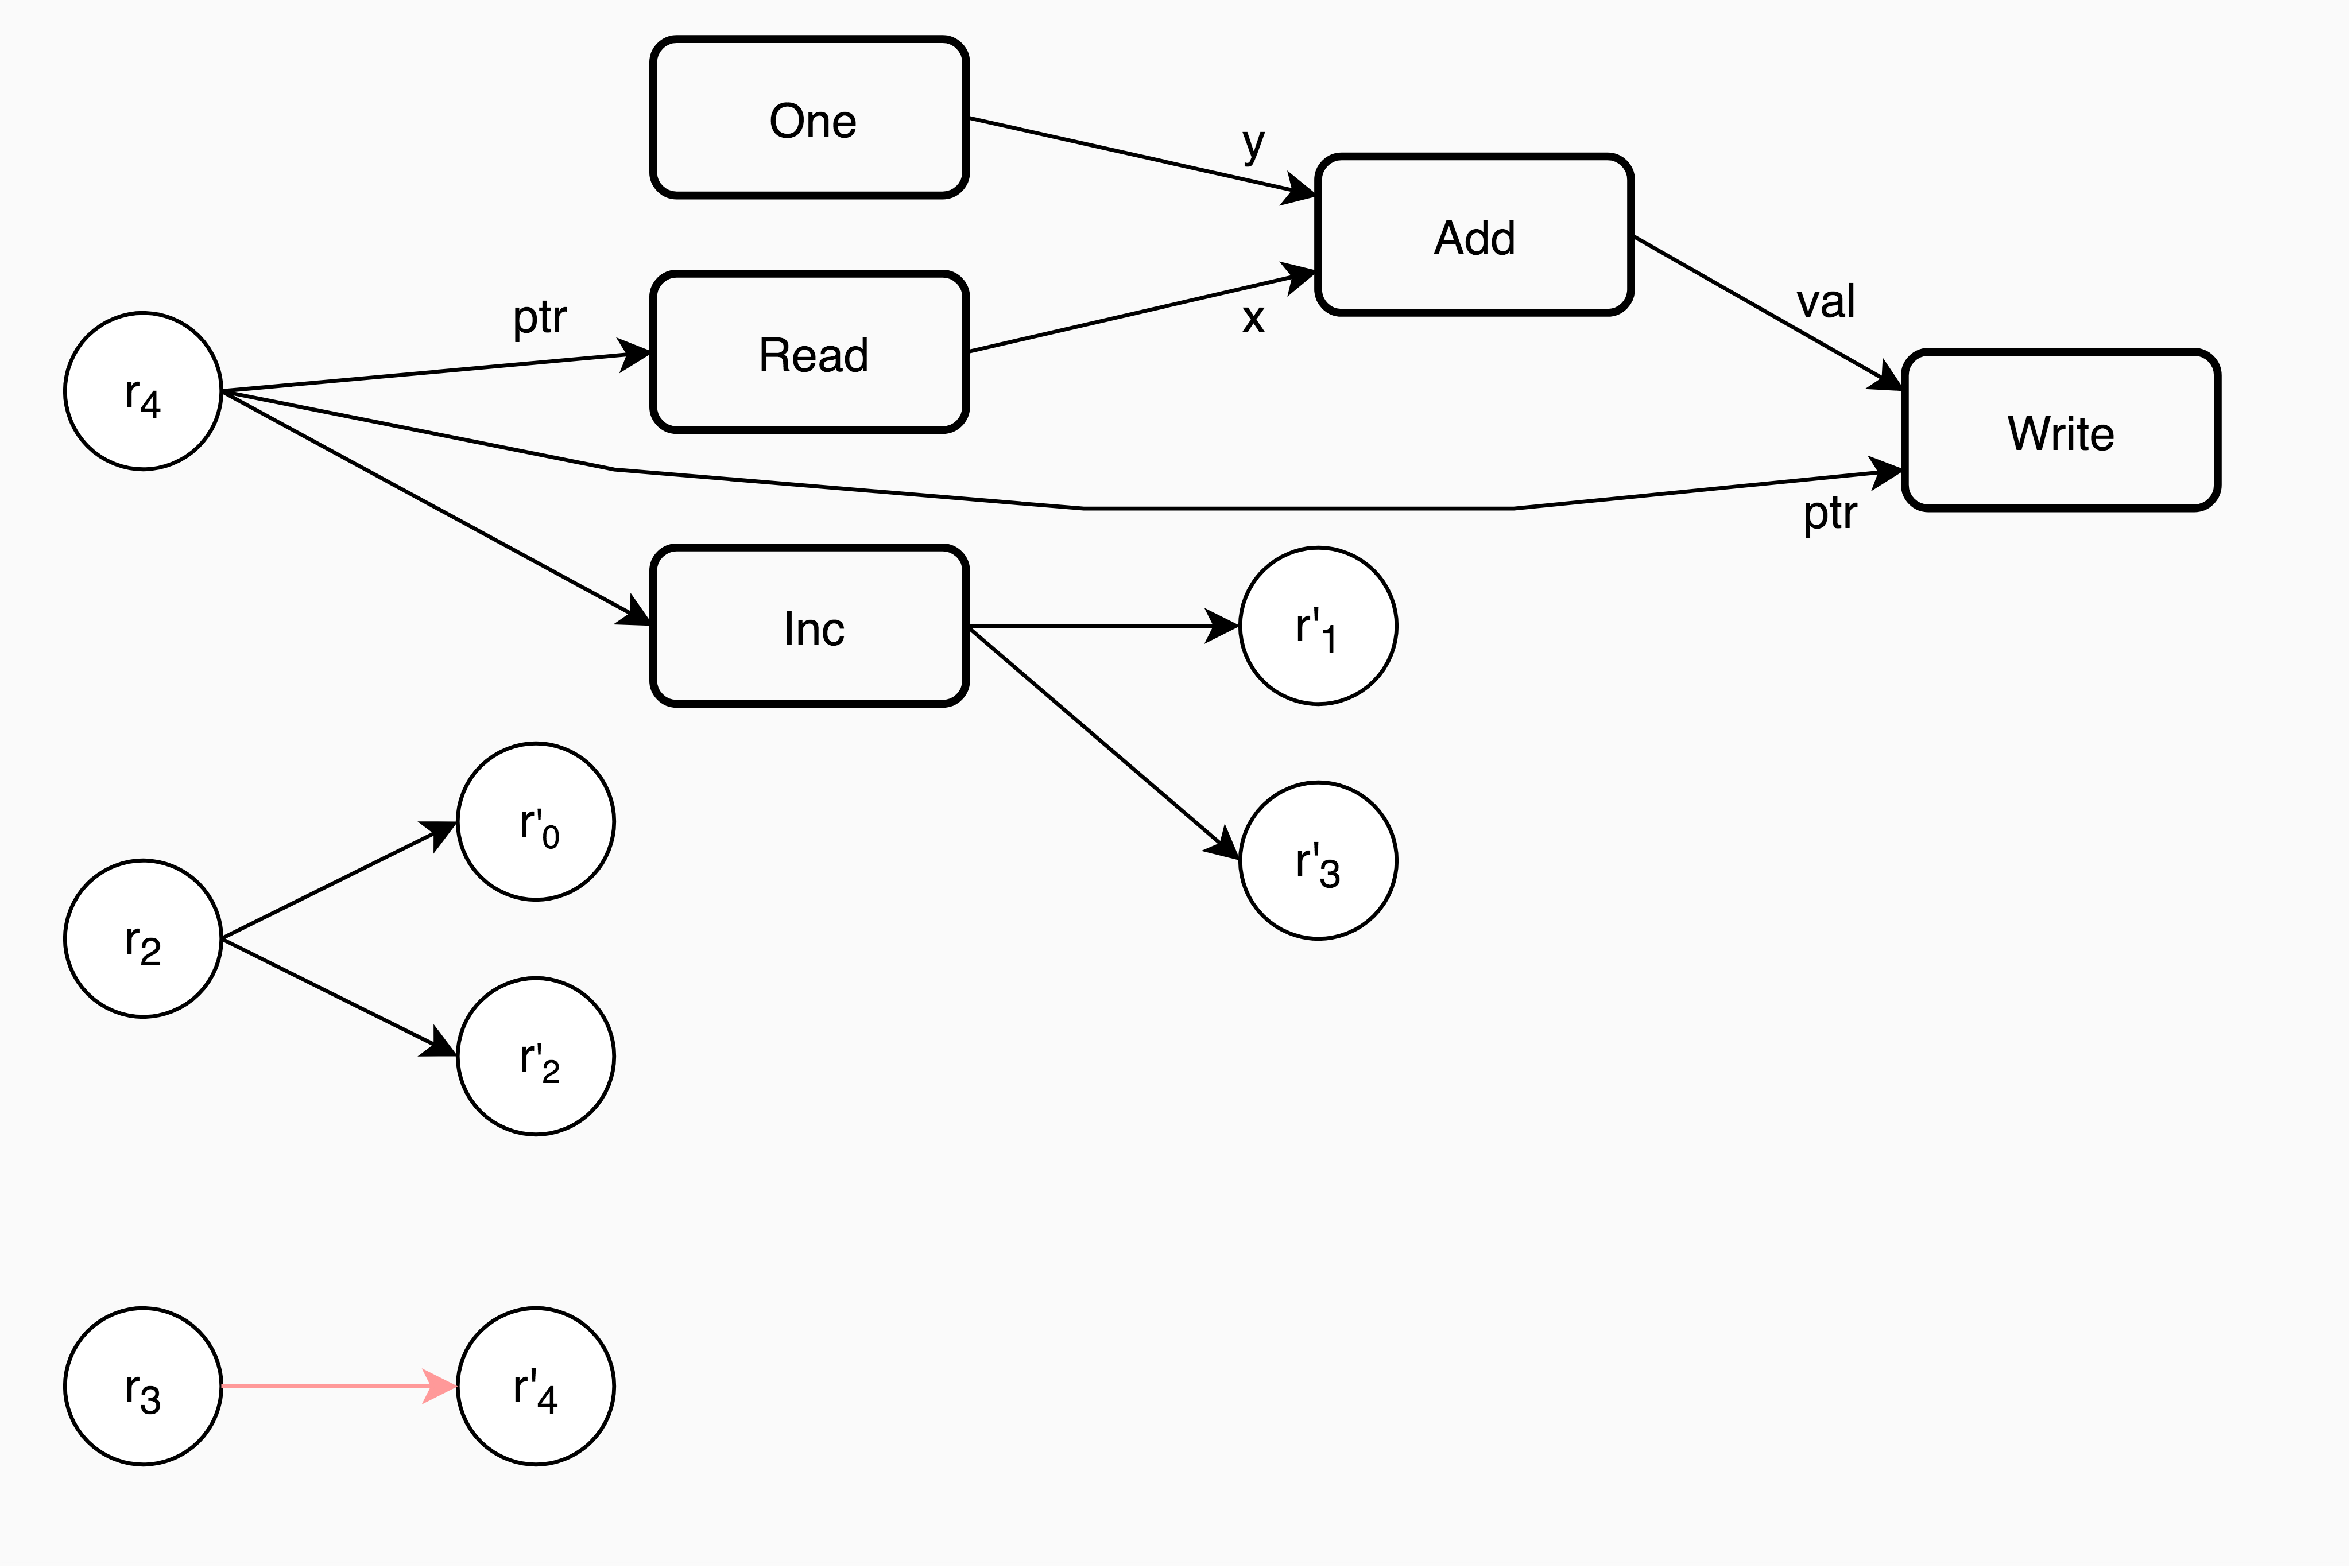
\includegraphics[width=\textwidth]{../figures/example-circuit-21.png}
  	\end{figure}
  \end{frame}
  \begin{frame}{Memory augmented version}
  	\begin{figure}
  		\centering
  		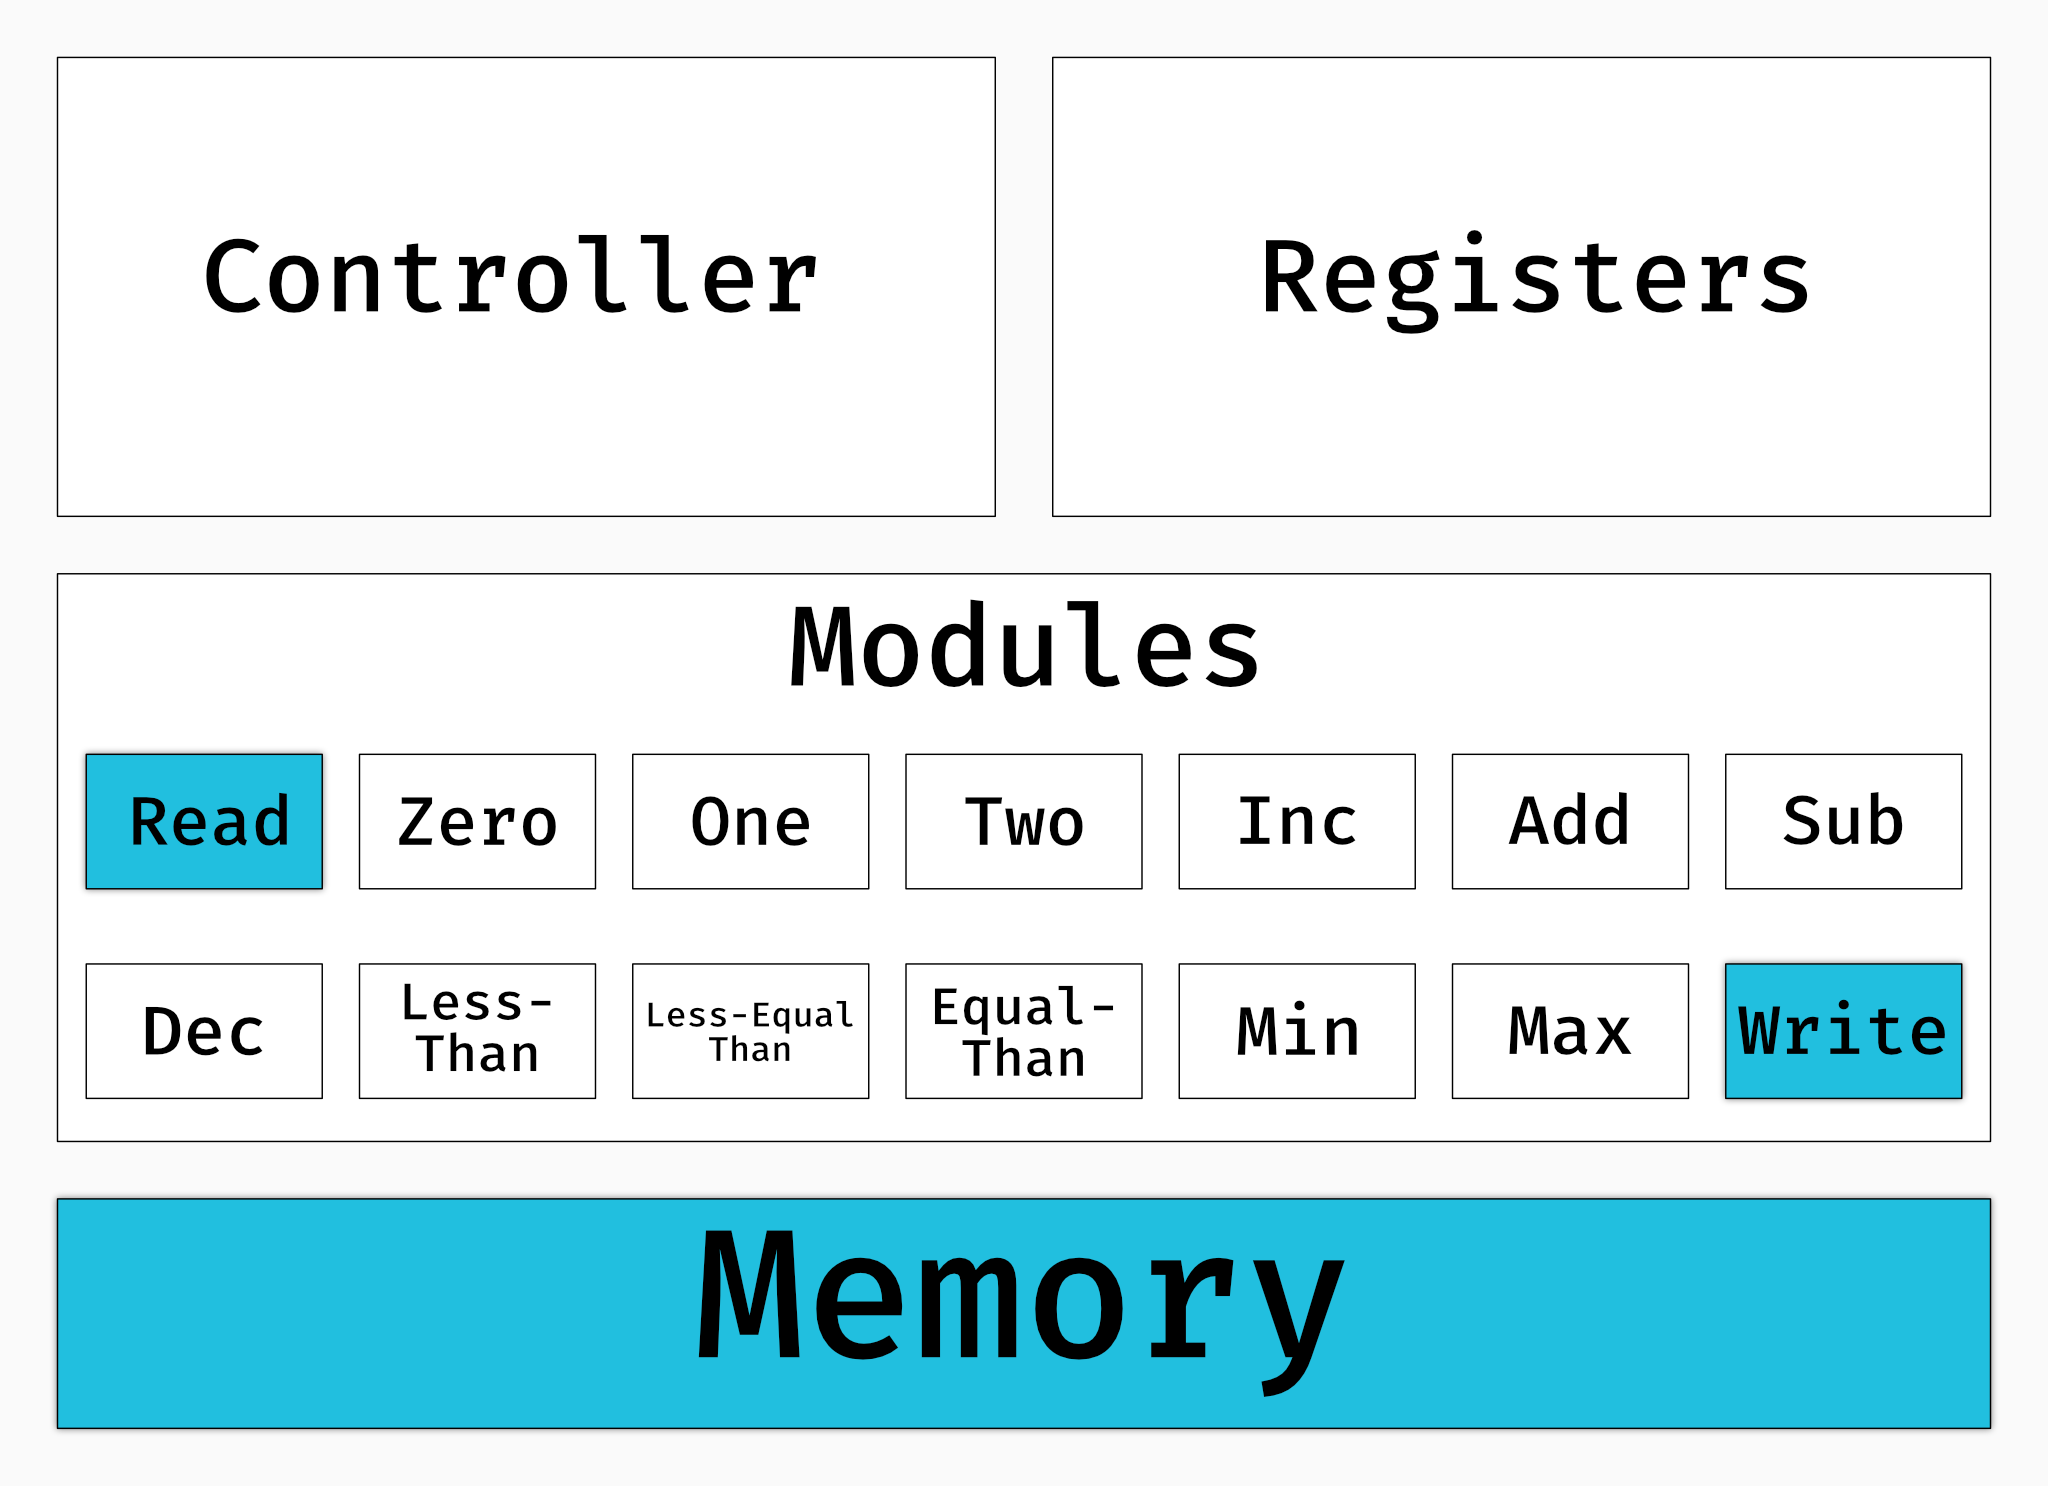
\includegraphics[width=\textwidth]{../figures/schema-nram-with-memory.png}
  	\end{figure}
  \end{frame}
  \begin{frame}{Memory}
  	The memory is a support of the Neural Random-Access Machines of $I$ memory cells, formalized as $\mathcal{M}\in\mathbb{R}^I_I$. Every value $\mathcal{M}_{i,j}$ is the probability that the $i^{th}$ cell contains the $j^{th}$ integer value of the set $N$.
  \end{frame}
  \begin{frame}{Read \& Write modules}
  	To interact with the memory, the NRAM has two further modules:
  	\begin{itemize}
  		\uncover<1->{
  			\item{\textbf{Read}: takes a pointer and returns $\mathcal{M}^Tp$. In other words, the value(s) pointed by the pointer.
			}
		}
		\uncover<2->{
			\item{\textbf{Write}: takes a pointer and a value, returns zero. Behave as follows:
				\begin{center}
					$\mathcal{M}=(J-p)J^T \cdot M+pa^T$
				\end{center}
				where $J\in{1}^I$ and $\cdot$ is the coordinate-wise multiplication. 
			}		
		}
  	\end{itemize}
  \end{frame}
  \begin{frame}{Timestep execution}
  	\begin{figure}
  		\centering
  		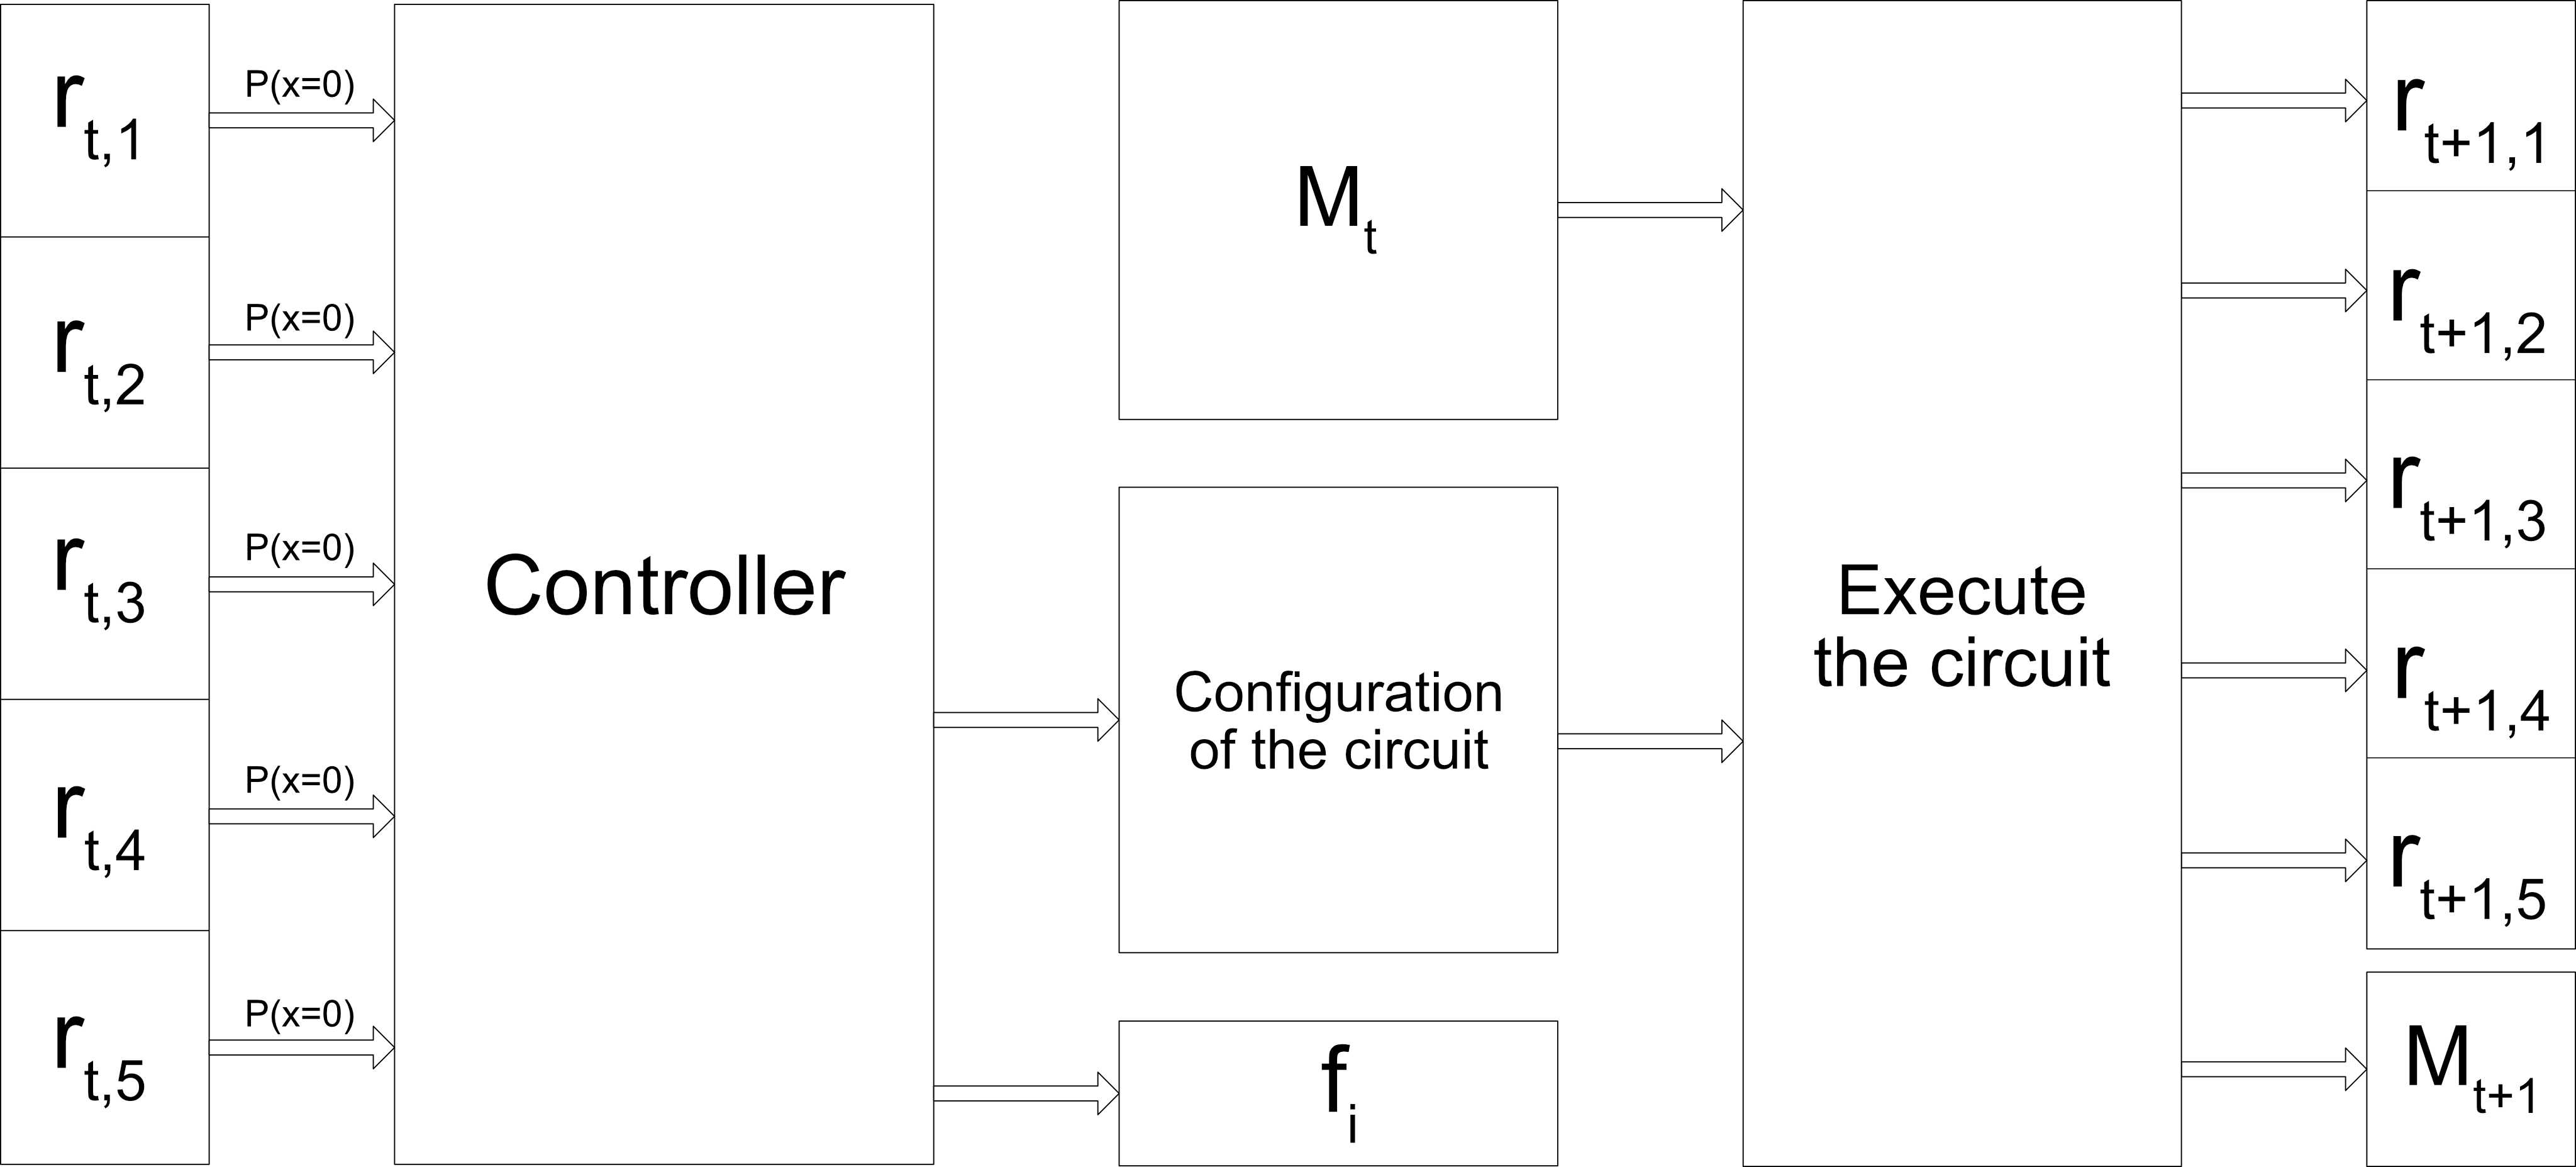
\includegraphics[width=\textwidth]{../figures/timestep-nram-execution.png}
  	\end{figure}
  \end{frame}
  \begin{frame}{Termination of NRAM}
  	The NRAM could terminate its execution in two ways:
  	\begin{itemize}
  		\uncover<1->{\item{Reaching the last timestep $T$}}
  		\uncover<2->{\item{Through its internal system of termination}}
  	\end{itemize}
  \end{frame}
  \begin{frame}{Internal system of termination}
  	NRAM uses a novel way of termination. In each timestep emits along the circuit configuration an $f_t = \sigma(x_i)$ which represents the willingness of terminating the execution. Although not specified in \cite{NRAM:2016}, we set the termination if $f_t \geq 1.0$. 
  \end{frame}
  \begin{frame}{Cost calculation}  
	Starting from $f_t$, the probability that the execution is not finished in the previous timestep is $\prod\limits_{i=1}^{t-1}(1 - f_{i})$, from which are computed
	  \begin{itemize}
	  	\uncover<1->{\item{the probability that the execution is produced in the current timestep
			\begin{center}
				$p_{t} = f_{t} \cdot \prod\limits_{i=1}^{t-1}(1 - f_{i})$
			\end{center}				  	
	  	}}
	  	\uncover<2->{\item{the probability that the execution is produced in the last timestep 
			\begin{center}
				$p_{T} = 1 - \sum\limits_{i=1}^{T-1}p_{i}$
			\end{center}	  	
	  	}}
	  \end{itemize}
  \end{frame}
  \begin{frame}{Cost calculation}
  	Let $\mathcal{M} \in \mathbb{R}^I_I$ the memory and $\mathcal{EM} \in N^I$, the expected negative log-likelihood is used as cost function and is defined as follows
  	\begin{center}
  		$-\sum\limits_{i=1}^{T}\Bigg(p_{t}\cdot\sum\limits_{i=1}^{|N|}log\Big(\mathcal{M}_{i, \mathcal{EM}_{i}}^{(t)}\Big)\Bigg)$
  	\end{center}
  \end{frame}
  \begin{frame}{Cost calculation - Example}
  	Let $t = 0$, $I = 4$ and $p_0 = 0.5$, we might have
  	\begin{table}
  		\centering
  		\begin{tabular}{ll}
  				\begin{tabular}{|c|c|c|c|}
					\multicolumn{4}{c}{Expected Memory} \\ \hline
					2 & 0 & 3 & 1 \\ \hline
					\multicolumn{4}{c}{} \\ 
					\multicolumn{4}{c}{Memory} \\ \hline
					0.3 & 0.2 & \cellcolor{mTableAlert}0.1 & 0.2 \\ \hline
					\cellcolor{mTableAlert}0.7 & 0.1 & 0.0 & 0.2 \\ \hline
					0.2 & 0.2 & 0.6 & \cellcolor{mTableAlert}0.0 \\ \hline
					0.1 & \cellcolor{mTableAlert}0.1 & 0.1 & 0.7 \\	 \hline		
  				\end{tabular} &
  			= \begin{tabular}{@{}c}$-(0.5 (\log(0.1) + \log(0.7) + $\\$\log(0.0 + \epsilon) + \log(0.1)) + \dots)$\end{tabular}
  		\end{tabular}
  	\end{table}
  \end{frame}
  \section{Artificial Neural Network}
  \begin{frame}{What are?}
  	The Artificial Neural Network are computing systems inspired by biology and belonging to classification techniques set. Classification systems learn patterns by view examples, i.e. approximate a function $f$ that maps example $x$ to the label $y$, where $(x, y) \in D$.
  \end{frame}
  \begin{frame}{Perceptron}
  	The most simple and old ANN \cite{ROSE:1958} is the Perceptron, formed as follows
  	\begin{figure}[t]
		\centering
		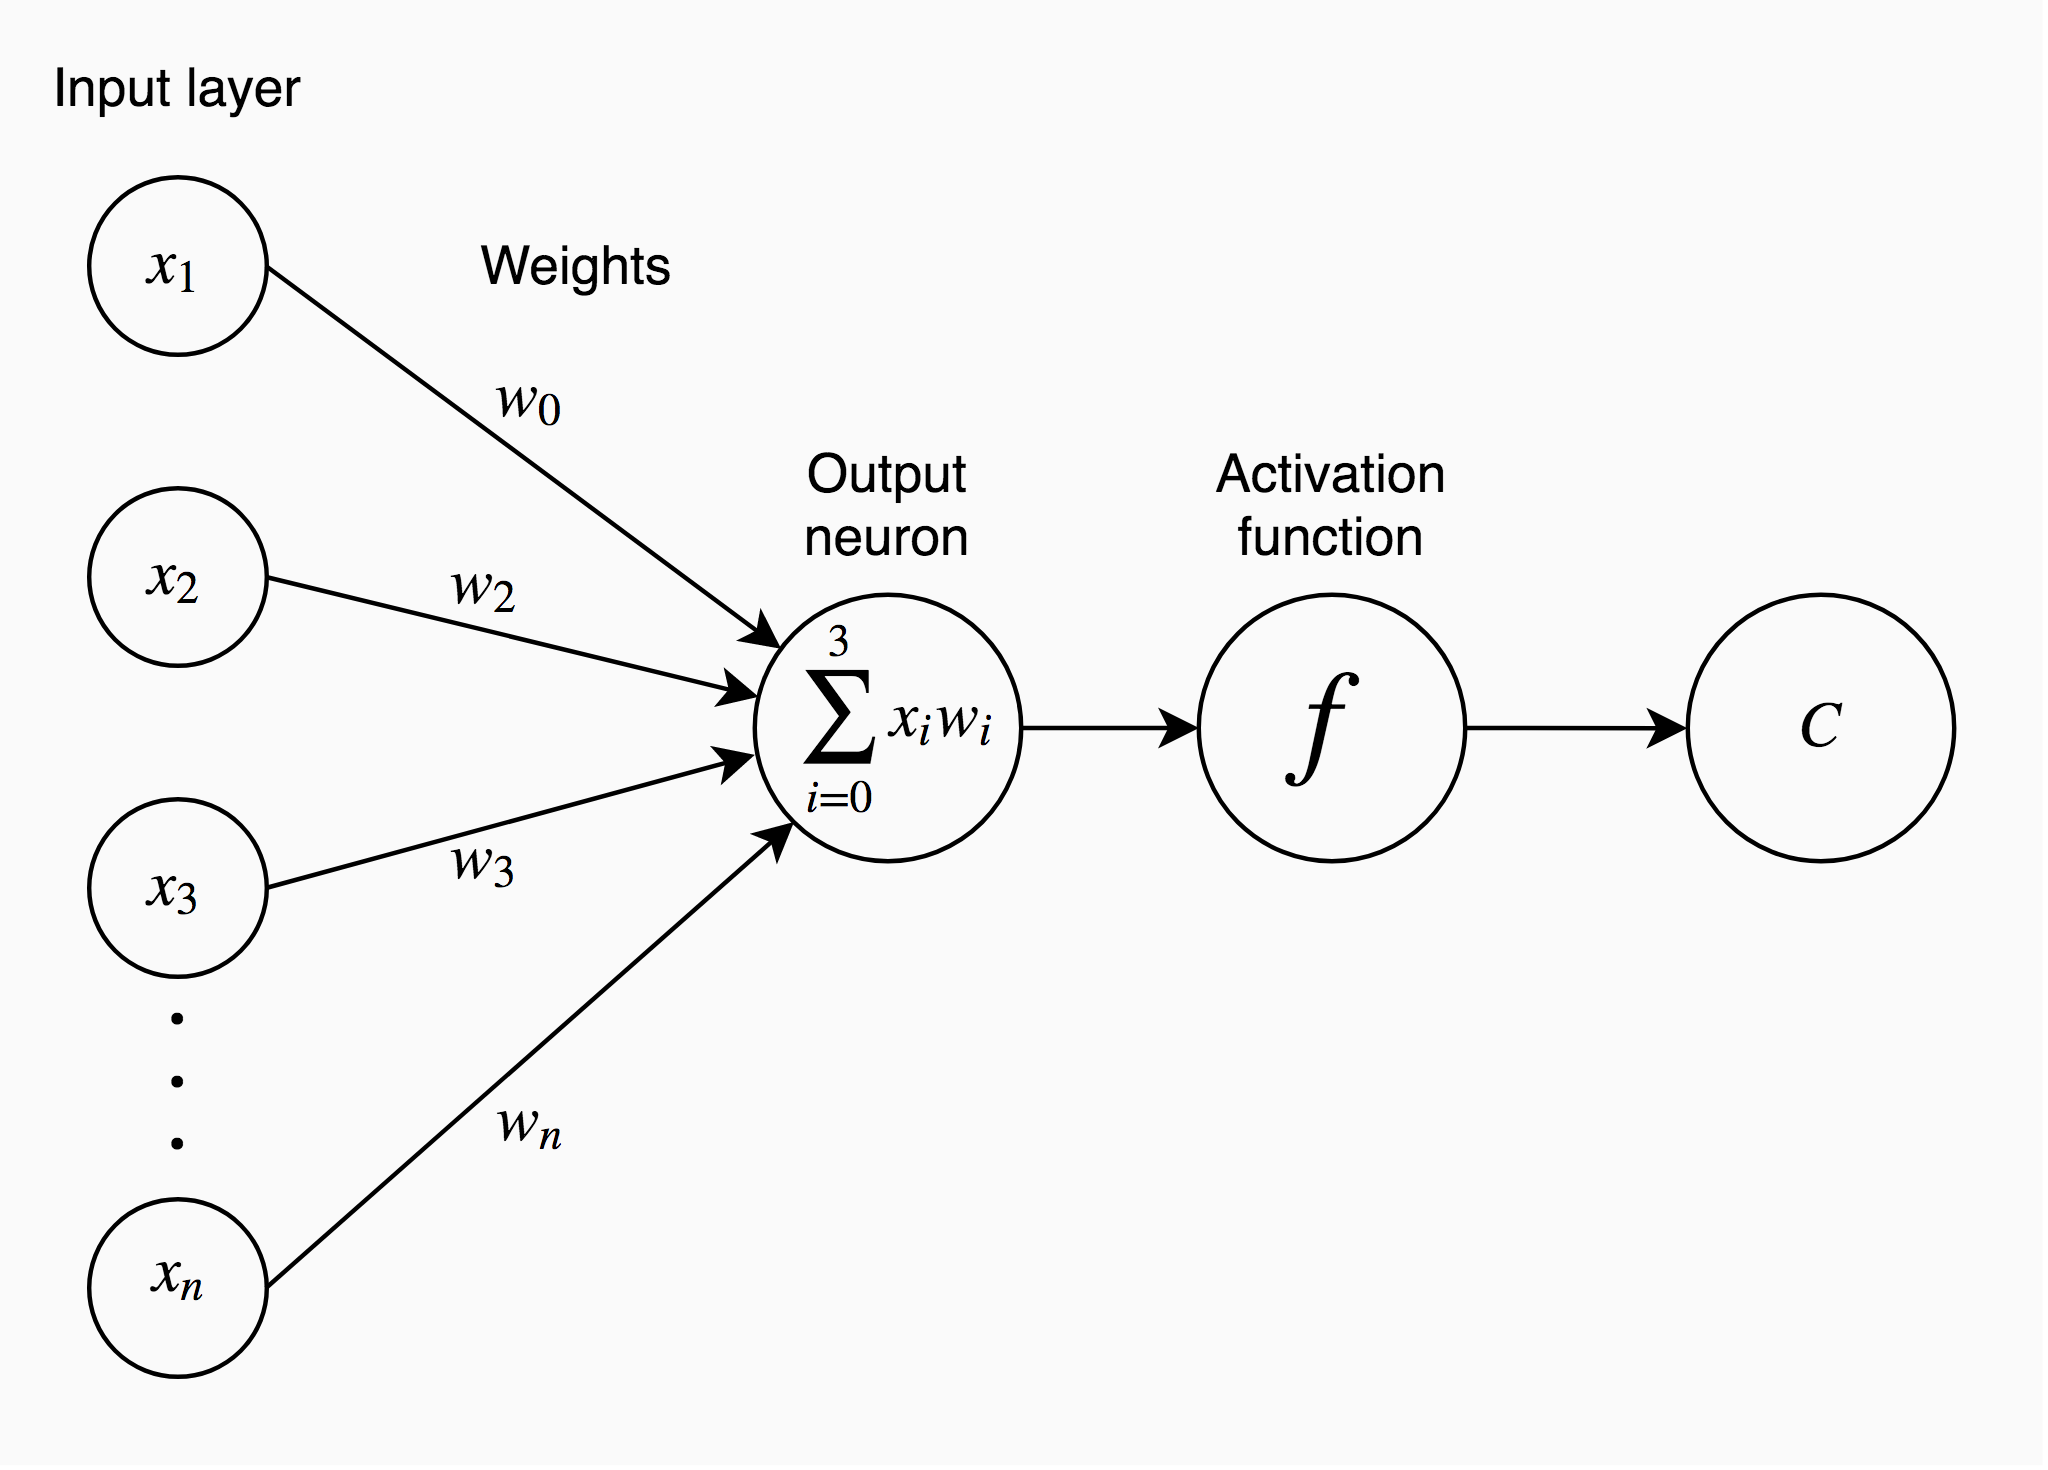
\includegraphics[width=0.8\textwidth]{../figures/perceptron.png}
	\end{figure}	
  \end{frame}
  \begin{frame}{Perceptron objective}
  	The Perceptron objective is to divide the examples in an hyperplane
  	\begin{figure}[t!]
		\centering		
		
		\resizebox{0.5\textwidth}{!}{\begin{tikzpicture}
			\begin{axis}[
    	    	 		grid=major, % Display a grid
    	    	  		grid style={dashed,gray!30}, % Set the style
				style={mark size=4pt},
  				xlabel={$x_1$},
  				ylabel={$x_2$},
  				xlabel style={below right},
  				ylabel style={above left},	
  				xmin = -10, xmax = 10,
  				ymin = -7, ymax = 11 
			]
				\addplot [only marks] table {first-samples.dat};
		
				\addplot [only marks, mark=o] table {second-samples.dat};
				\addplot [domain=-20:20, samples=2, dashed] {x + 2.5};
      		\end{axis}
		\end{tikzpicture}}
		\caption{Example with only two features, $x_1$ and $x_2$, and two classes, represented by the black and white circles.}
		
	\end{figure}
  \end{frame}
  \begin{frame}{Multi Layer Perceptron (MLP)}
  	An evolution of the Perceptron is the Multi Layer Perceptron, formed as follows
  	\begin{figure}[t]
		\centering
		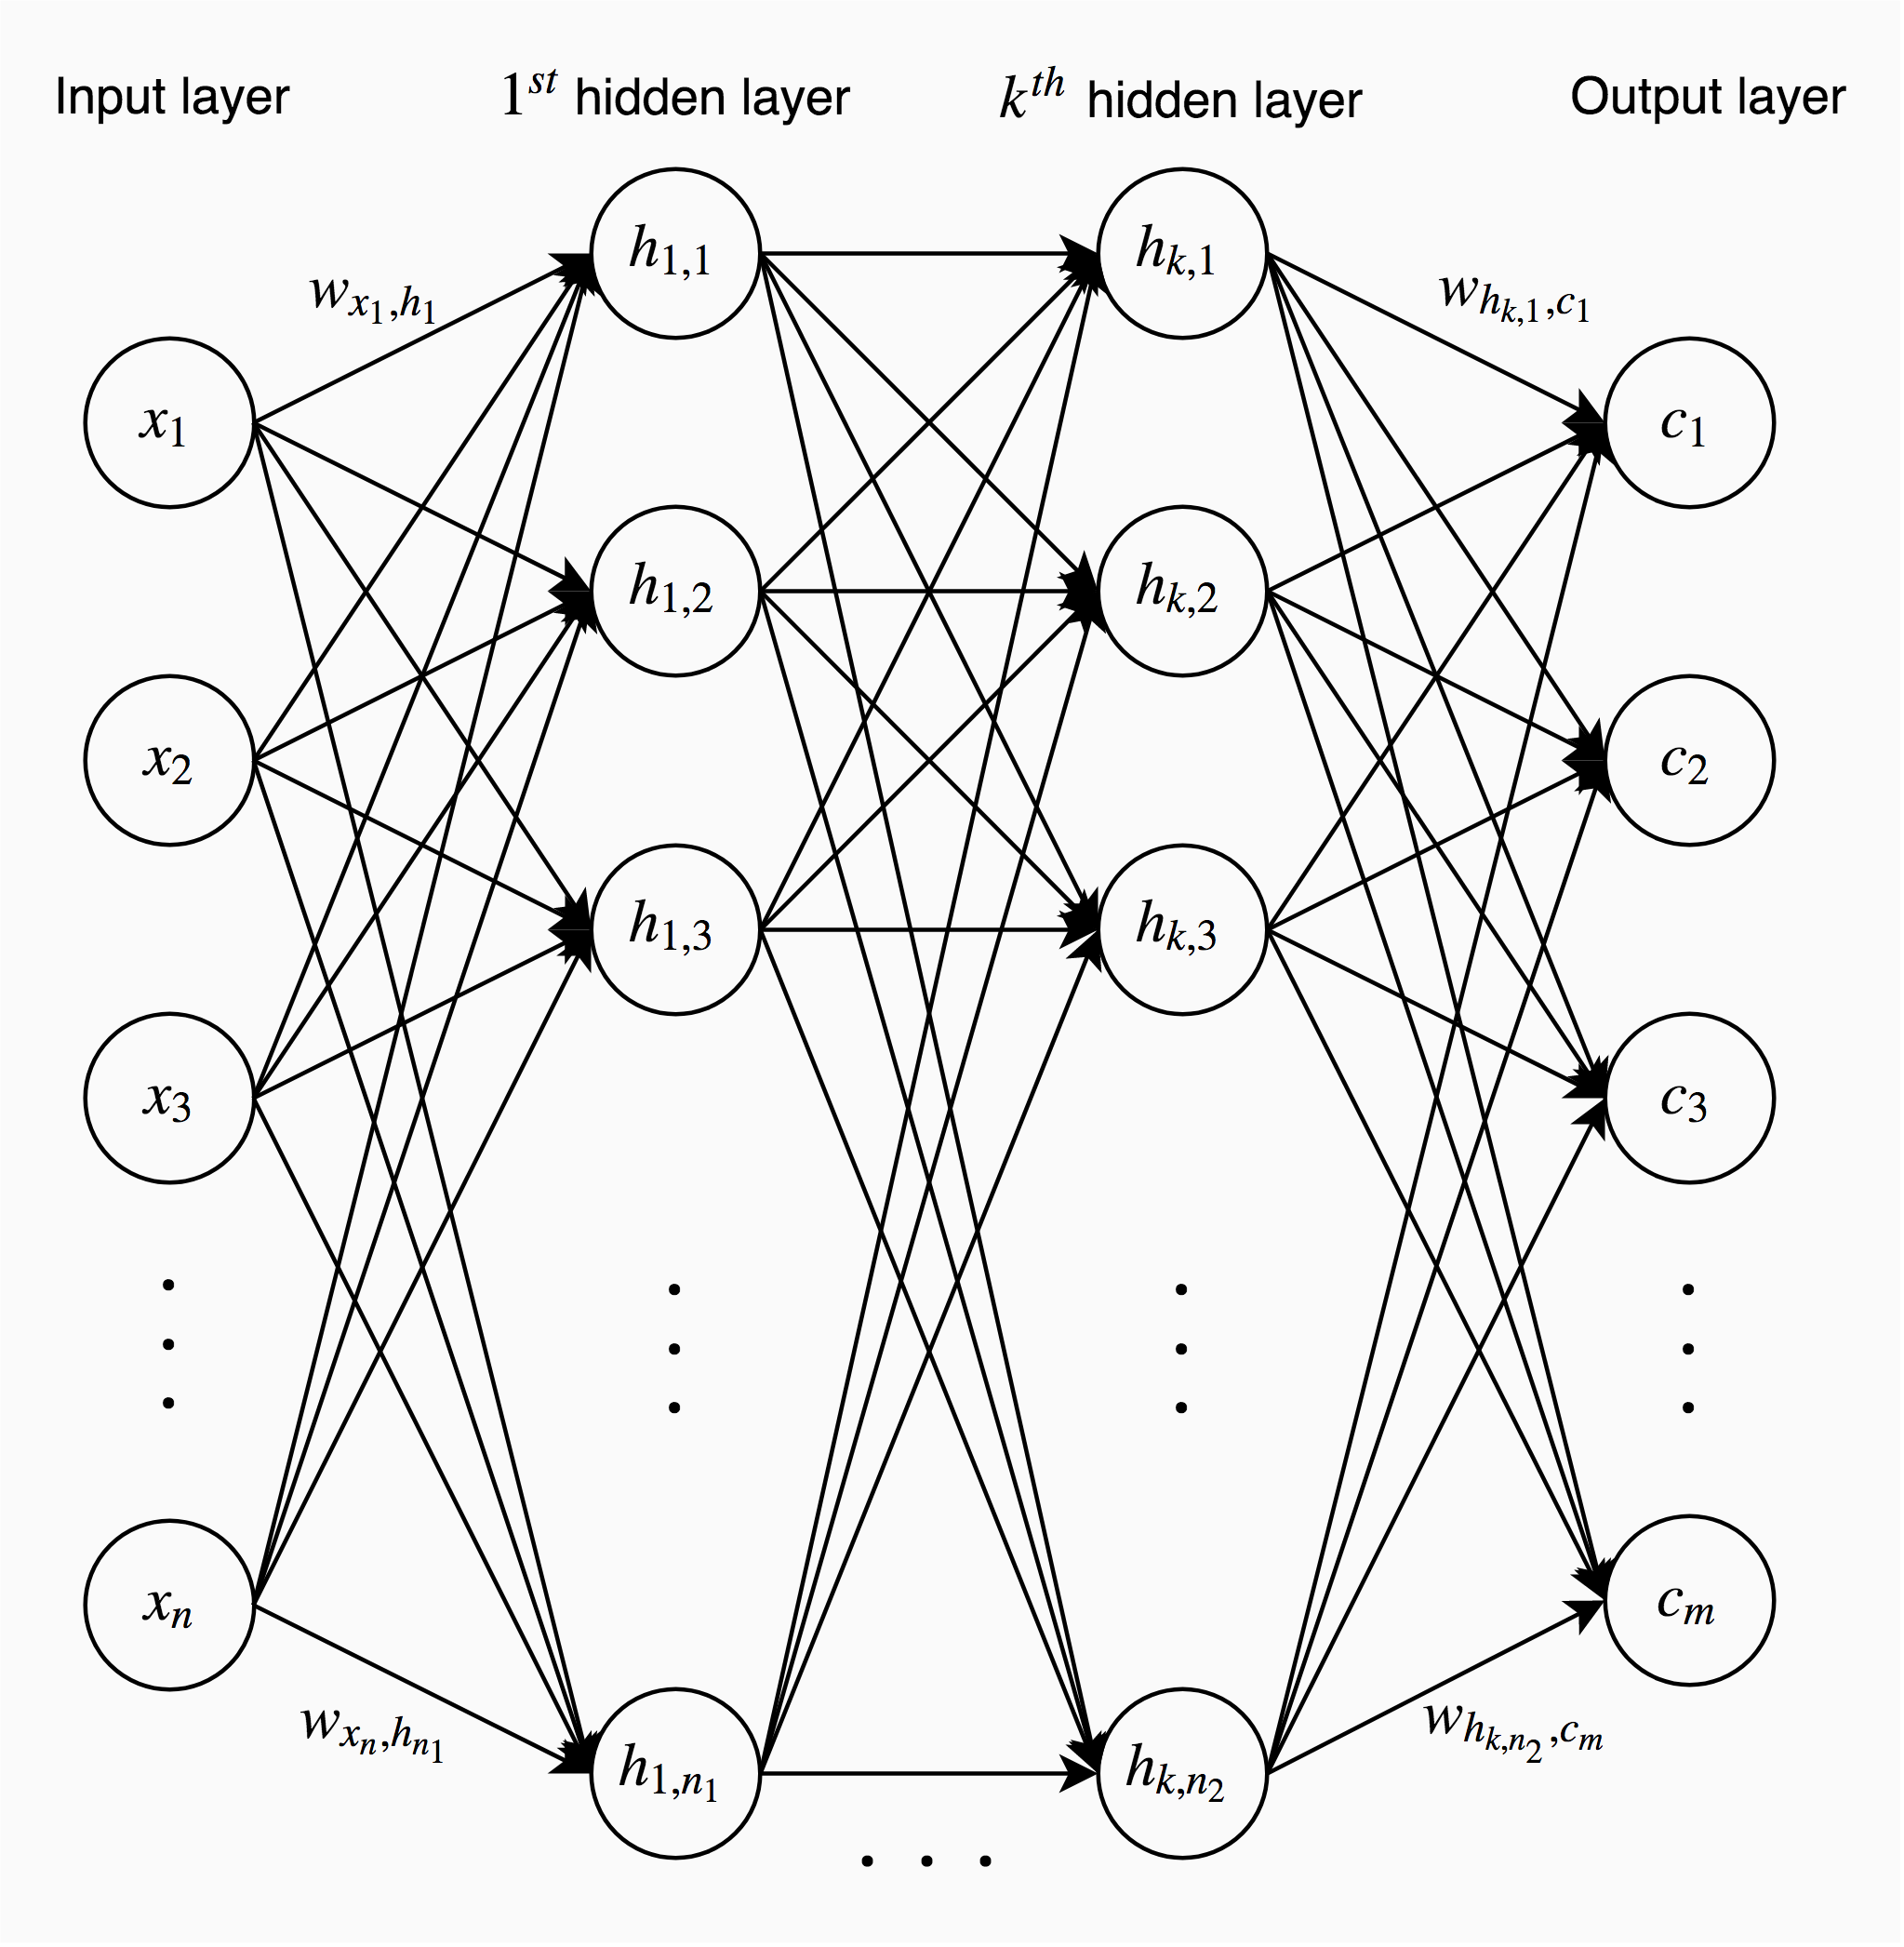
\includegraphics[width=0.6\textwidth]{../figures/multi-layer-perceptron.png}
	\end{figure}	
  \end{frame}
  \begin{frame}{Training of an ANN}
  	The training of an ANN follows two steps:
  	\begin{itemize}
  		\uncover<1->{\item{The initialization of the weights/parameters}}
  		\uncover<2->{\item{The re-computation of these searching to minimize the value of an objective function}}
  	\end{itemize}
  \end{frame}
  \begin{frame}{Gradient Descent \& back-propagation}
  	\begin{minipage}{0.475\textwidth}One method to search a optimal/sub-optimal configuration of the parameters through the minimization of the cost function through the Gradient Descent and the back-propagation, with a behaviour similar to the descent of a bowl by an hypothetical ball, where the bowl bottom corresponds to the global minimum of the function.
  	\end{minipage}
  	\hfill
  	\begin{minipage}{0.475\textwidth}
  		\begin{figure}
  	
		\definecolor{GDFirst}{RGB}{203,62,63}
		\definecolor{GDSecond}{RGB}{238,138,112}
		\definecolor{GDThird}{RGB}{245,191,113}
		\definecolor{GDFourth}{RGB}{221,220,220}
		\definecolor{GDFiveth}{RGB}{179,205,249}
		\definecolor{GDSixth}{RGB}{129,165,247}
		\definecolor{GDSeventh}{RGB}{82,110,215}
  		\begin{tikzpicture}[samples=100,smooth,scale=0.7]
			\begin{scope}
				\draw[opacity=0,fill=GDFirst,fill opacity=1] plot[domain=0:360] ({cos(\x)*sqrt(20/(sin(2*\x)+2))},{sin(\x)*sqrt(20/(sin(2*\x)+2))});
				\draw[opacity=0,fill=GDSecond,fill opacity=1] plot[domain=0:360] ({cos(\x)*sqrt(16/(sin(2*\x)+2))},{sin(\x)*sqrt(16/(sin(2*\x)+2))});
				\draw[opacity=0,fill=GDThird,fill opacity=1] plot[domain=0:360] ({cos(\x)*sqrt(12/(sin(2*\x)+2))},{sin(\x)*sqrt(12/(sin(2*\x)+2))});
				\draw[opacity=0,fill=GDFourth,fill opacity=1] plot[domain=0:360] ({cos(\x)*sqrt(8/(sin(2*\x)+2))},{sin(\x)*sqrt(8/(sin(2*\x)+2))});
				\draw[opacity=0,fill=GDFiveth,fill opacity=1] plot[domain=0:360] ({cos(\x)*sqrt(4/(sin(2*\x)+2))},{sin(\x)*sqrt(4/(sin(2*\x)+2))});
				\draw[opacity=0,fill=GDSixth,fill opacity=1] plot[domain=0:360] ({cos(\x)*sqrt(1/(sin(2*\x)+2))},{sin(\x)*sqrt(1/(sin(2*\x)+2))});
				\draw[opacity=0,fill=GDSeventh,fill opacity=1] plot[domain=0:360] ({cos(\x)*sqrt(0.0625/(sin(2*\x)+2))},{sin(\x)*sqrt(0.0625/(sin(2*\x)+2))});
			
				\draw[->,blue,ultra thick] (-2,3.65) to (-1.93,3);
				\draw[->,blue,ultra thick] (-1.93,3) to (-1.75,2.4);
				\draw[->,blue,ultra thick] (-1.75,2.4) to (-1.5,1.8);
				\draw[->,blue,ultra thick] (-1.5,1.8) to (-1.15,1.3);
			\end{scope}
		\end{tikzpicture}
  	\end{figure}
  	\end{minipage}
  \end{frame}
  \begin{frame}{Back-propagation}
  	The search of those minima is done firstly through the computing of the ANN gradient through the back-propagation, which it is divided into two phases:
  	\begin{itemize}
  		\uncover<1->{\item{Forward propagation}}
  		\uncover<2->{\item{Backward propagation}}
  	\end{itemize}
  \end{frame}
  \begin{frame}{Forward phase}
  	\begin{figure}
  		\centering
  		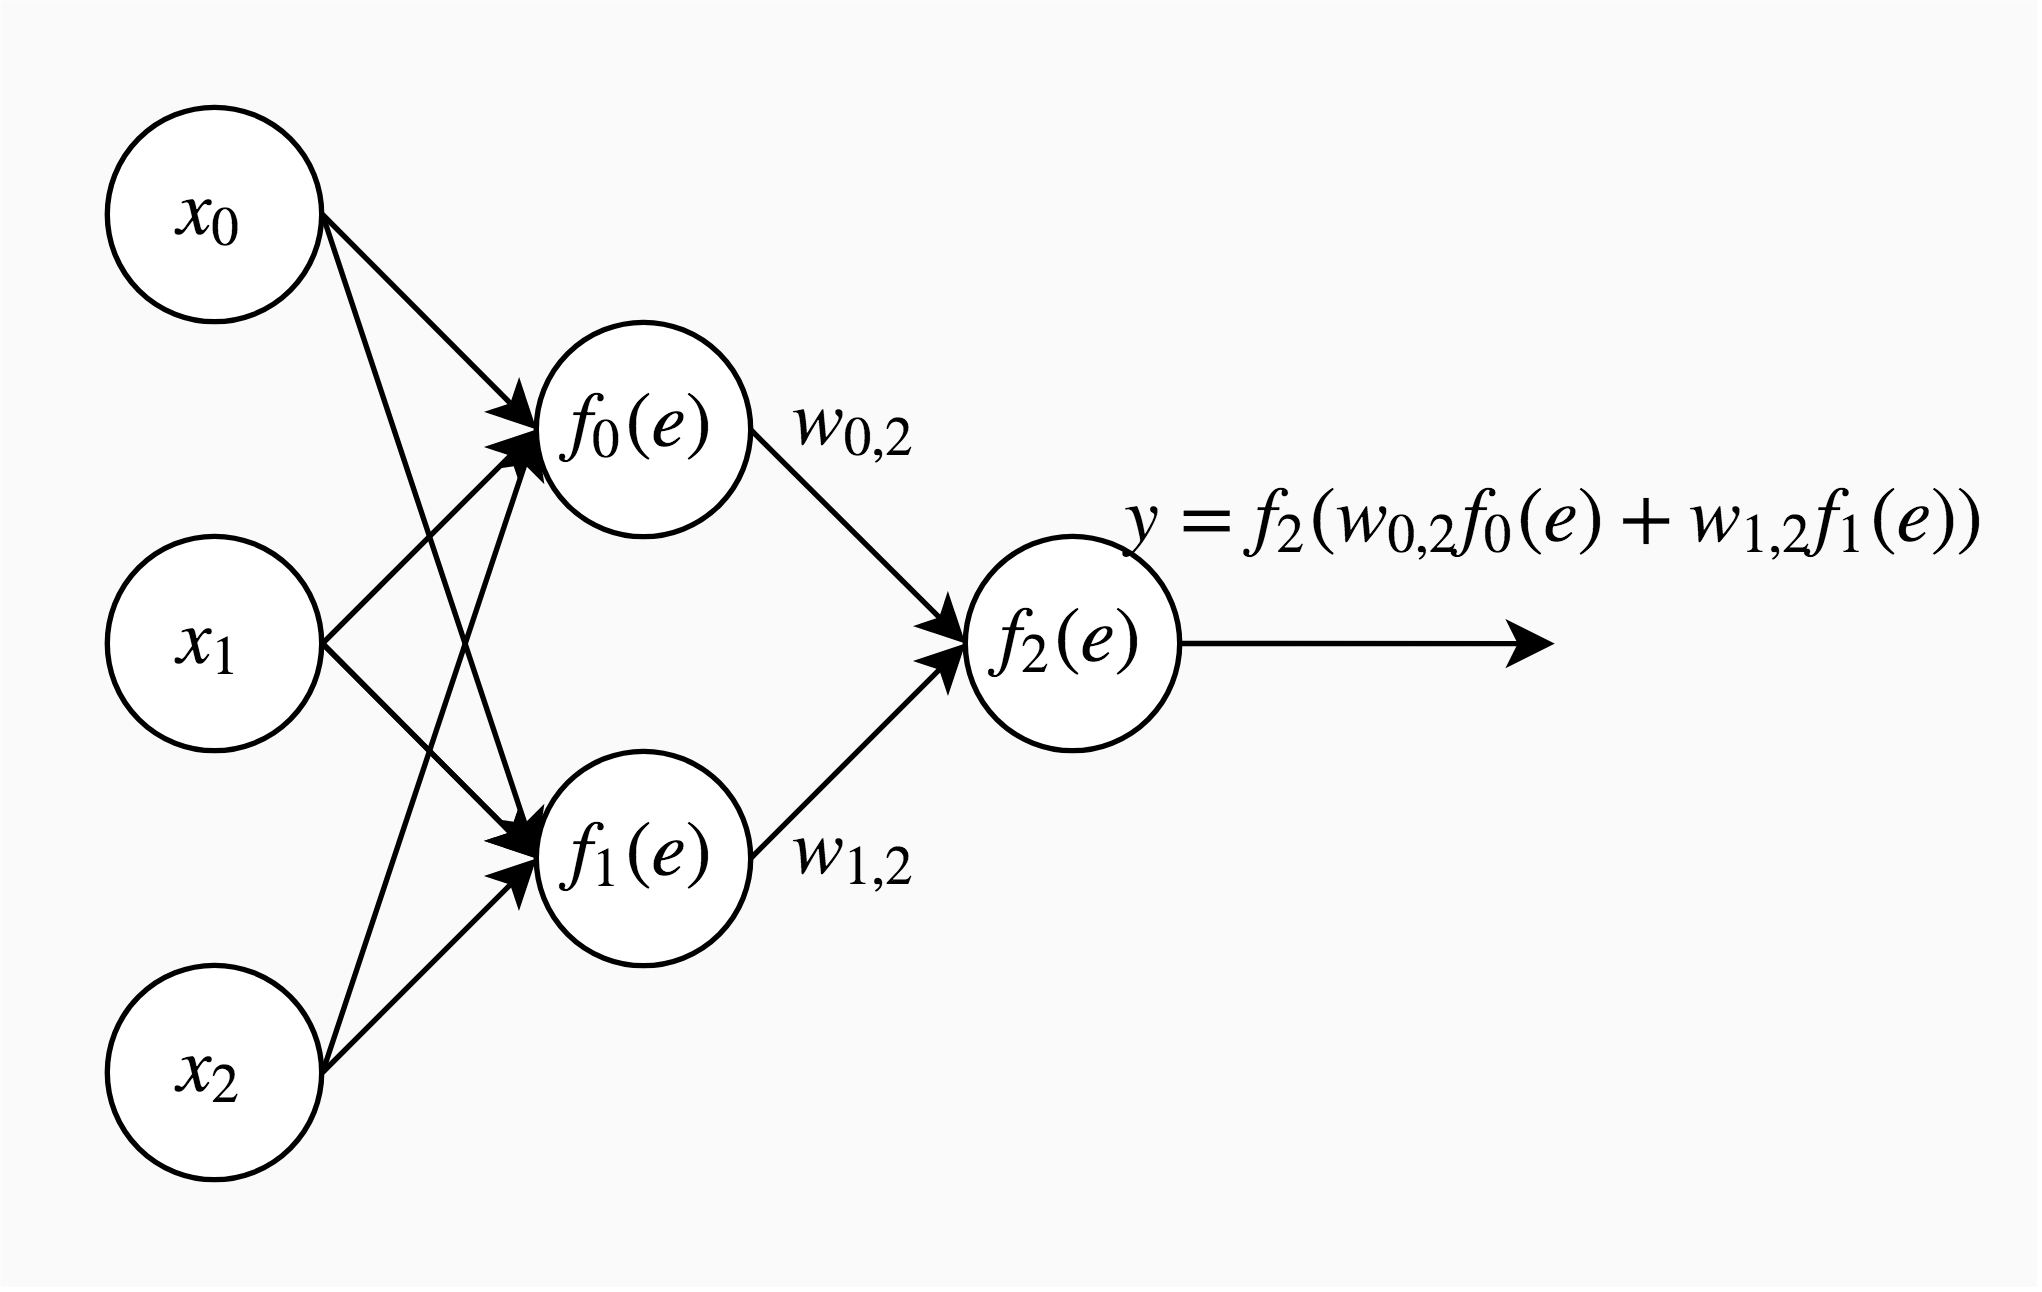
\includegraphics[width=0.8\textwidth]{../figures/forward-propagation.png}
  		\caption{Last pass of forward phase, when the output of ANN is computed}
  	\end{figure}
  \end{frame}
  \begin{frame}{Backpropagation phase}
  	\begin{figure}
  		\centering
  		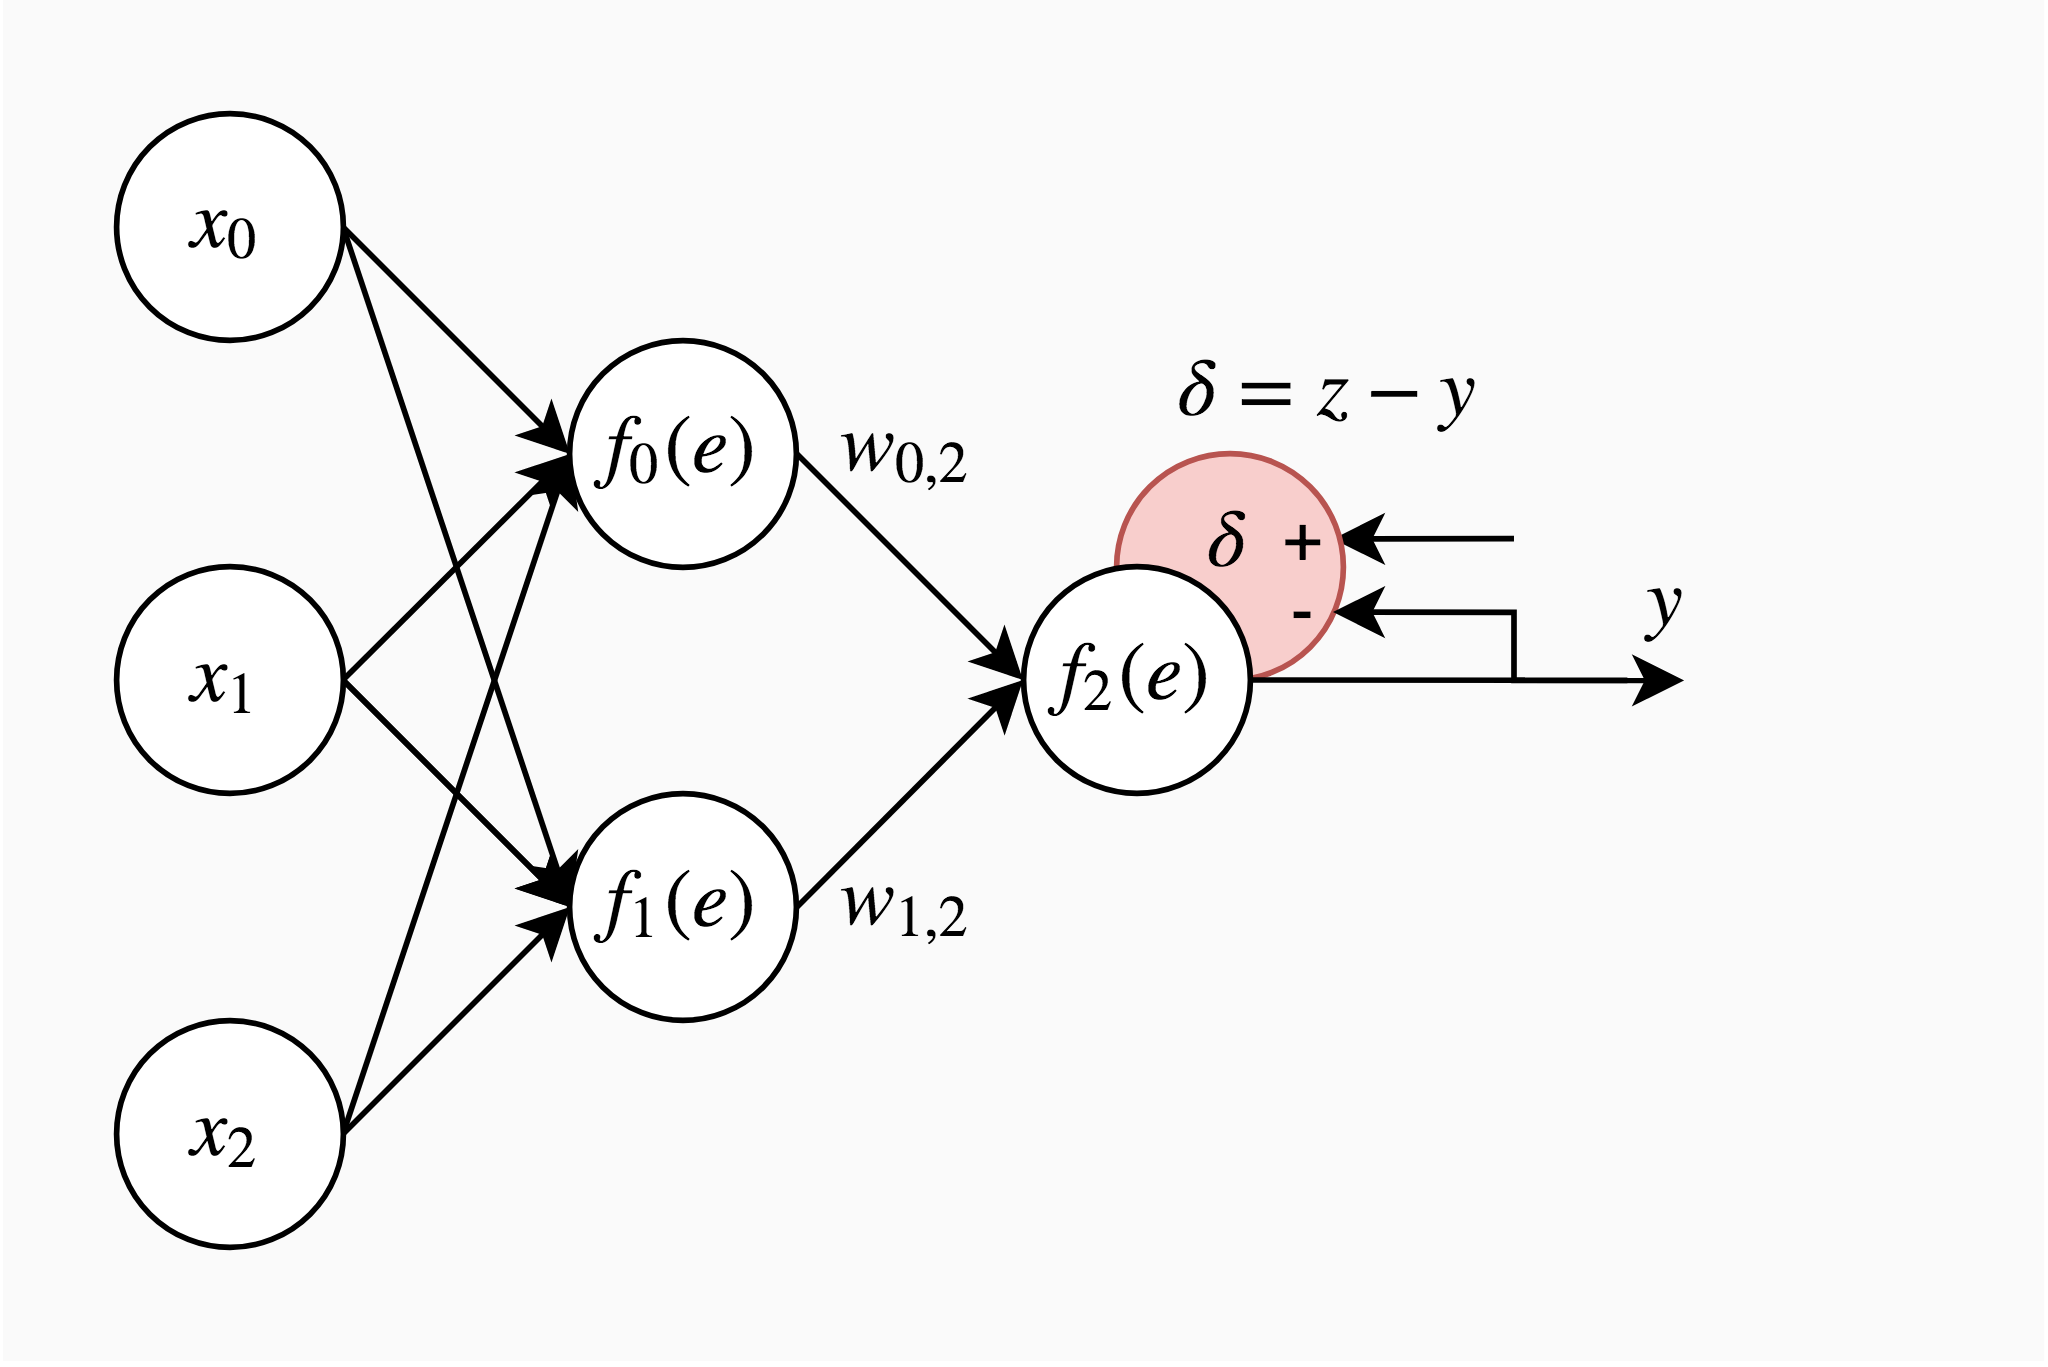
\includegraphics[width=0.8\textwidth]{../figures/backward-propagation-0.png}
  		\caption{Computing of $\delta$. It can be computed directly because is available a class that can be compared to the ANN exit.}
  	\end{figure}
  \end{frame}
  \begin{frame}{Backpropagation phase}
  	\begin{figure}
  		\centering
  		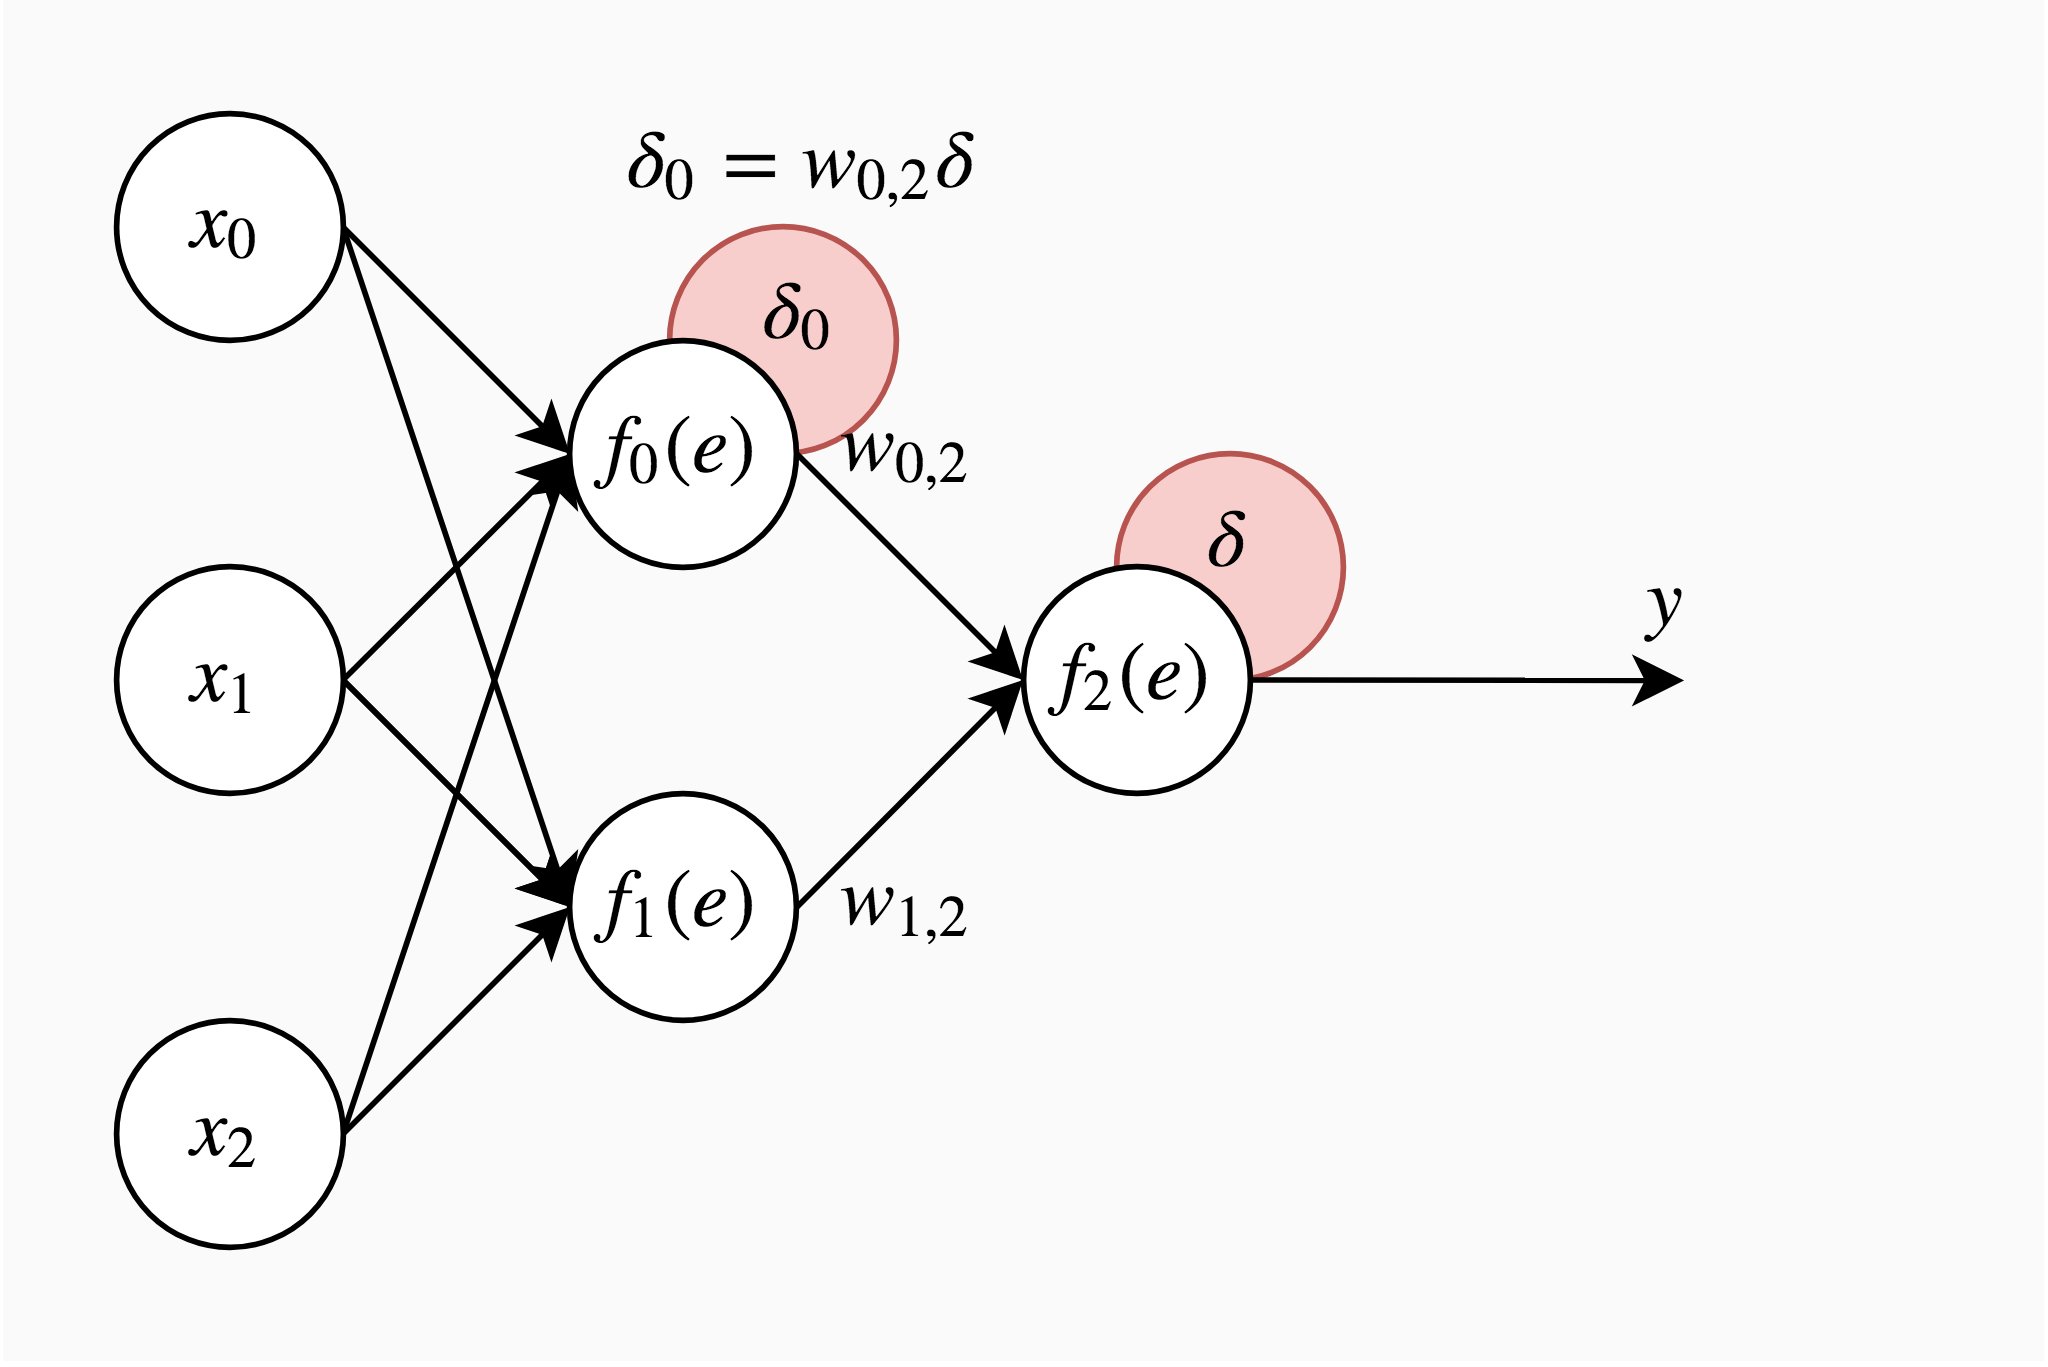
\includegraphics[width=0.8\textwidth]{../figures/backward-propagation-1.png}
  		\caption{Computing of $\delta_0$ using $\delta$.}
  	\end{figure}
  \end{frame}
  \begin{frame}{Backpropagation phase}
  	\begin{figure}
  		\centering
  		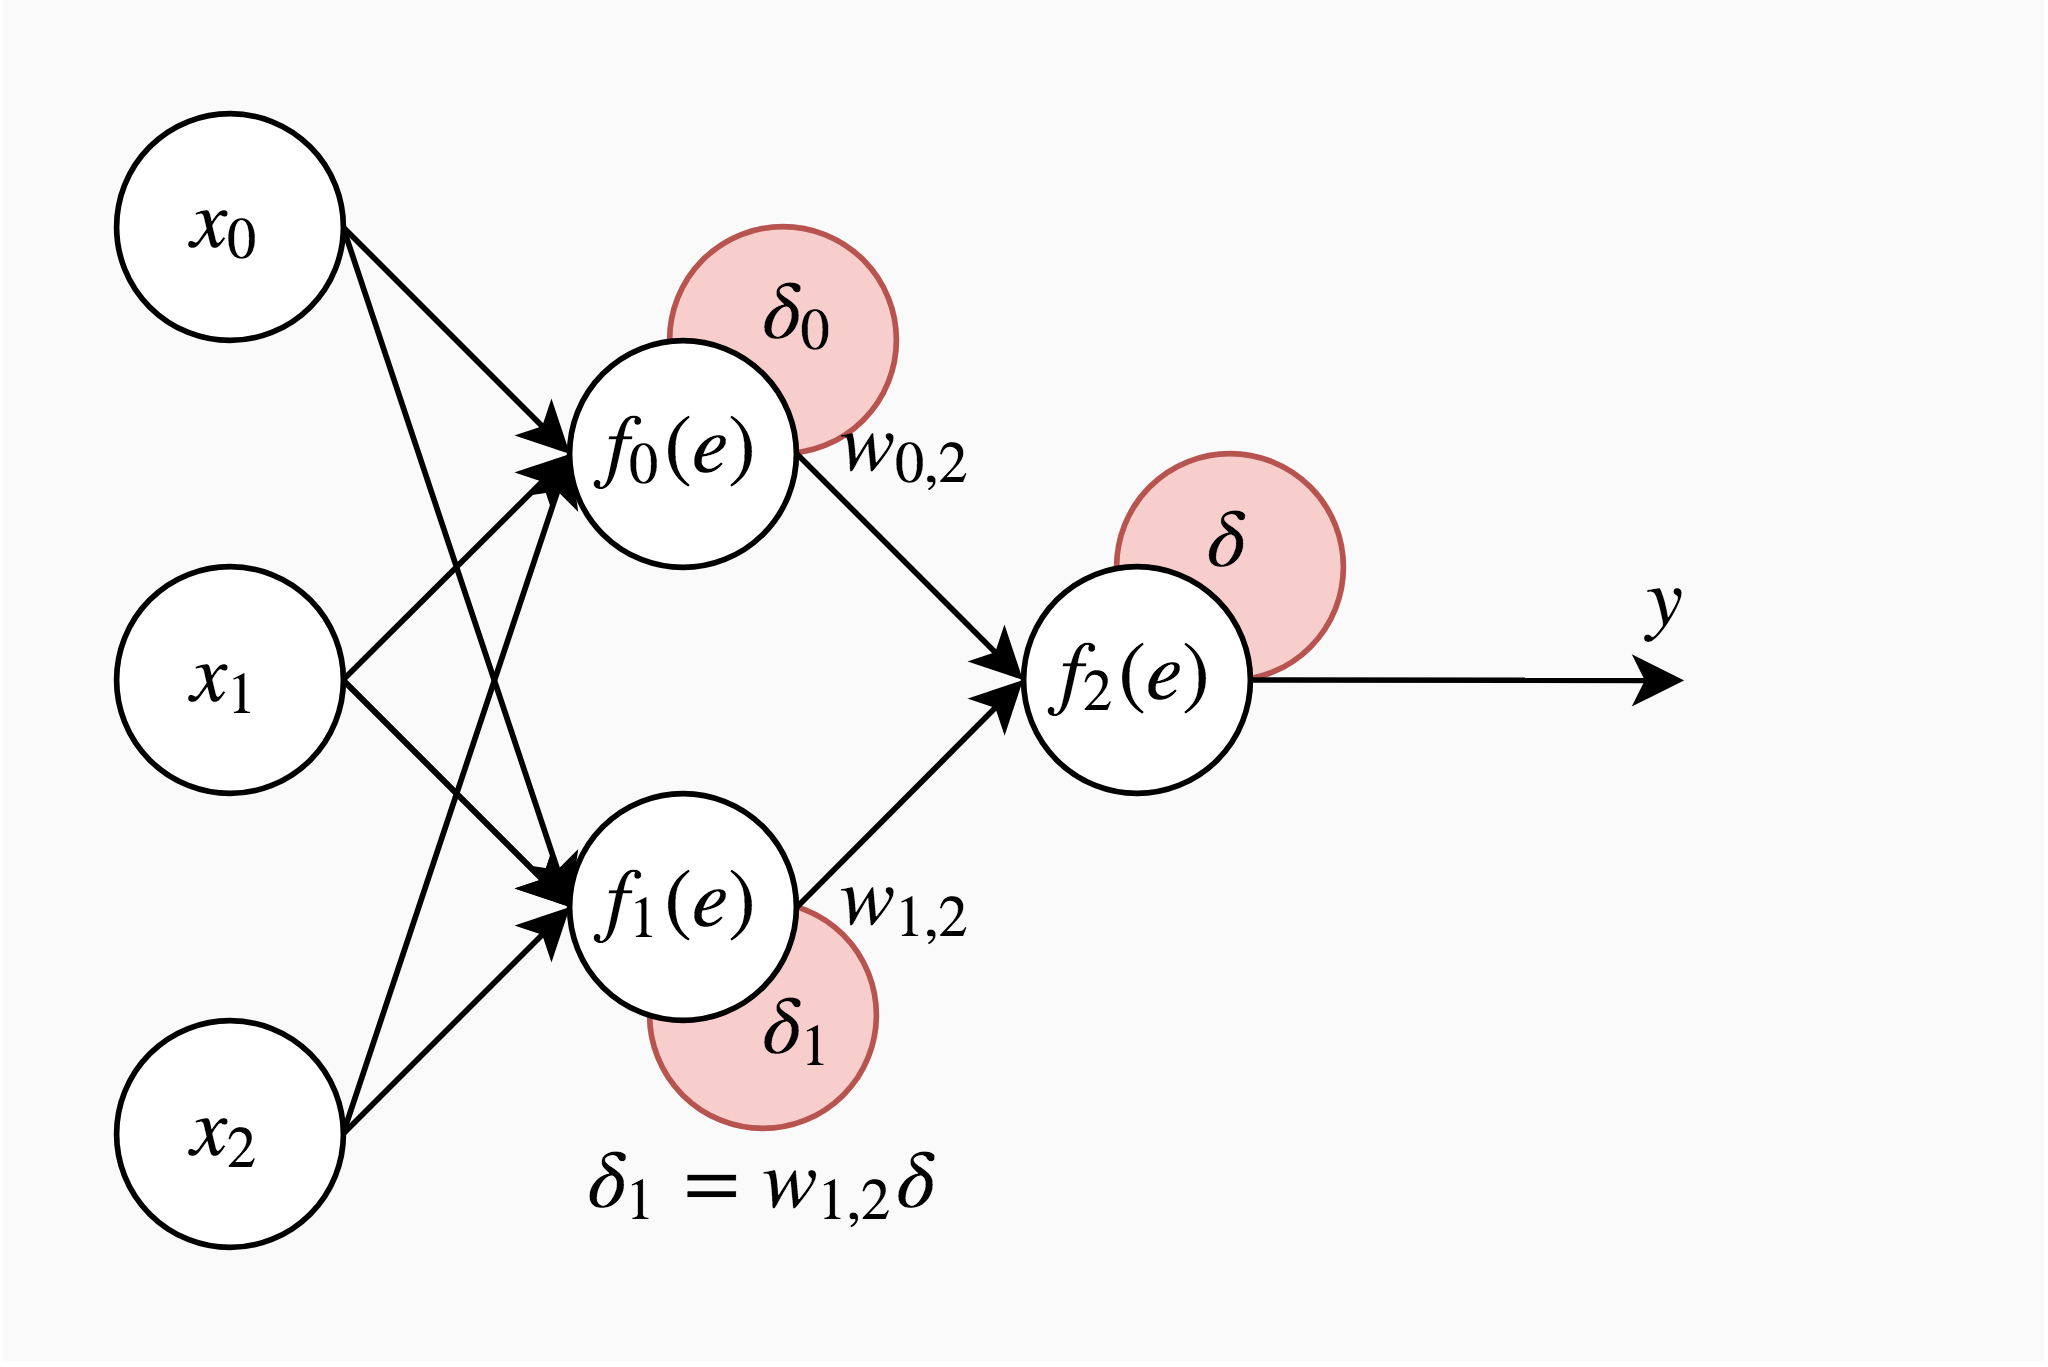
\includegraphics[width=0.8\textwidth]{../figures/backward-propagation-2.png}
  		\caption{Computing of $\delta_1$ using $\delta$.}
  	\end{figure}
  \end{frame}
  \begin{frame}{Gradient Descent \& ADAM}
  	ADAM is a gradient-based optimization algorithm that uses the concept of momentum to regularize the descent of the gradient.
  \end{frame}
  \begin{frame}{ADAM}
  	Let $\beta_1$ and $\beta_2$ two exponential decay rates used for the momentum estimates, $\epsilon$ a small real-valued scalar, $\lambda$ the learning rate and $w_{ij}$ the reference weight. The steps to update a parameter are the following
  	\begin{itemize}
  		\uncover<1->{\item{\textbf{Compute $m_{ij}^{(t)}$}: \(m_{ij}^{(t)} = \beta_1m_{ij}^{(t-1)} + (1 - \beta_1)\delta_{ij}^{(t)}\)}}
  		\uncover<2->{\item{\textbf{Compute $v_{ij}^{(t)}$}: \(v_{ij}^{(t)} = \beta_2v_{ij}^{(t-1)} + (1 - \beta_2)\delta_{ij}^{2,  (t)}\)}}
  		\uncover<3->{\item{\textbf{Regularize $m_{ij}^{(t)}$ w.r.t. $\beta_1$:} $\hat{m}_{ij}^{(t)} = \frac{m_{ij}^{(t)}}{1 - \beta_{1}}$}}
  		\uncover<4->{\item{\textbf{Regularize $v_{ij}^{(t)}$ w.r.t. $\beta_2$:} $\hat{m}_{ij}^{(t)} = \frac{m_{ij}^{(t)}}{1 - \beta_{1}}$}}
  		\uncover<5->{\item{\textbf{Update $w_{ij}^{(t)}$:} $w_{ij}^{(t)} = w_{ij}^{(t)} - \lambda\frac{\hat{m}_{ij}^{(t)}}{\sqrt{\hat{v}_{ij}^{(t)}} + \epsilon}$}}
  	\end{itemize}
  \end{frame}
  \section{Differential Evolution \& DENN}
  \begin{frame}{Description}
  	Differential Evolution (DE) is a metaheuristic introduced in \cite{DESEHGOCS:1997}, belonging to the family of Evolutionary Algorithms (EAs), that has as objective the searching of a solution through the parallel evolution of a set of candidate solutions. 
  	
  	This set is defined as \textbf{population} and it is composed by NP D-dimensional numerical vectors where each of them is called individual, chromosome or genoma.
  \end{frame}
  \begin{frame}{Description}
  	Its functioning is iterative and after a first phase of initialization of the individuals the following step is executed
  	\begin{itemize}
  		\uncover<1->{\item{\textbf{Mutation}}}
  		\uncover<2->{\item{\textbf{Crossover}}}
  		\uncover<3->{\item{\textbf{Selection}}}
  	\end{itemize}
  \end{frame}
  \begin{frame}{Mutation}
  	Through the mutation phase a new population, called donor set, is created. Let $x$ an individual at the generation $G$, also called target. A donor is generated combining $x$ with some other individuals through a differential mutation operator. 
  \end{frame}
  \begin{frame}{Mutation - Example}
  	For example, the method \textbf{rand/1} work as follows 
  	\begin{center}
		$v_{i,G+1} = x_{r_{1},G} + F\cdot(x_{r_{2},G} - x_{x_{3},G})$
	\end{center}
	where $r_{1},r_{2},r_{3} \in \{1,2,\dots,NP\}$ are mutually exclusive indices and $F$ is a real-valued constant defined by the user.
  \end{frame}
  \begin{frame}{Crossover}
  	The Crossover phase does nothing else than mixing up one-by-one the donor vectors components with the target vectors with some crossover methods, generating the \textbf{trials} vectors set and enhancing the potential diversity of the population (a better exploration). 
  \end{frame}
  \begin{frame}{Crossover - Example}
  	For example, let the target vector $x_{i,G}$ and the mutant $v_{i,G}$ the \textbf{bin} strategy work as follows
\begin{align}
	u_{ji, G} = \begin{cases}
		v_{ji,G}, & \textrm{if}\ (\textit{randb}(j) \leq \textit{CR})\ \textrm{or}\ j=\textit{rnbr}(i)\\
		x_{ji,G}, & \textrm{if}\ (\textit{randb}(j) > \textit{CR})\ \textrm{and}\ j\neq\textit{rnbr(i)}
	\end{cases} & i=1,2,\dots,D
\end{align}
where  $\textit{randb}(j)$ is a function which generate a real-valued number for the $j^{th}$ parameter according to binomial distribution, $\textrm{CR}\in[0,1]$ is the global user-defined crossover constant used as a threshold and $\textit{rnbr}(i)$ is a function that generate a random index which ensures that is selected at least one parameter of the mutant $v_{i}$.
  \end{frame}
  \begin{frame}{Selection}
	Each trial is compared one-by-one to the corresponding target using the fitness function - if the target have a smaller cost with respect to the trial, than it is retained as individual of the population of the next generation and vice-versa.
  \end{frame}
  \begin{frame}{Differential Evolution variants}
  	There exist various DE variants; some of these that are used in the thesis are
  	\begin{itemize}
  		\uncover<1->{\item{\textbf{JADE}: generate for each target $x_i$, $\textrm{F}_i$ and $\textrm{CR}_i$ with an adaptation system which is based on two memories of \textit{infinite} size called $S_{\textrm{F}}$ and $S_{\textrm{CR}}$;}}
  		\uncover<2->{\item{\textbf{SHADE}: generate for each target $x_i$, $\textrm{F}_i$ and $\textrm{CR}_i$ with an adaptation system which is based on two memories of \textit{finite} size $M_{\textrm{F}}$ and $M_{\textrm{CR}}$ called \textit{historical memories};}}
  		\uncover<3->{\item{\textbf{L-SHADE}: similar to SHADE, but bases is function also in a linear reduction of the population.}} 
  	\end{itemize}
  \end{frame}
  \begin{frame}{Mutation variants}
  	
  \end{frame}
  \begin{frame}{Crossover variants}
  	
  \end{frame}
  \begin{frame}{DENN (Differential Evolution for Neural Network)}
  
  \end{frame}
  \section{Implementation and results}
  \begin{frame}{Implementation}
  	\begin{figure}
  		\centering
  		\includegraphics[width=0.4\textwidth]{../figures/nram-implementation.png}
  		\caption{Three implementations were developed: the first two are used to train the controllers and the last is used to test the generalization ability of the discovered controllers.}
  	\end{figure}
  \end{frame}
  \begin{frame}{Datasets}
  	The datasets used during the training are automatically generated at runtime. Each batch of samples is composed by:
	\begin{itemize}
		\item{initial memories: the memories which are manipulated by NRAM during the execution;}
		\item{expected memories: the memories which are compared to the modified initial memories for cost computation;}
		\item{cost masks: used to take into account only parts of the memories during the computing of the cost;}
		\item{error rate masks: used to take into account only parts of the memories during the computing of the error rate;}
	\end{itemize}
  \end{frame}
  \begin{frame}{Problems}
  	The following are some of the problems introduced in \cite{NRAM:2016}:
  	\begin{itemize}
  		\uncover<1->{\item{\textbf{Access}}}
  		\uncover<2->{\item{\textbf{Increment}}}
  		\uncover<3->{\item{\textbf{Copy}}}
  		\uncover<4->{\item{\textbf{Reverse}}}
  	\end{itemize}
  \end{frame}
  \begin{frame}{Access}
	Given a value $k$ and an array \textbf{A}, return $\textbf{A}[k]$. Input is given as $k,\ A[0],\ \dots,\ $\\$\textbf{A}[n-1],\ \textit{NULL}$ and the network should replace the first memory cell with $\textbf{A}[k]$. 
	\begin{table}[h!]
		\centering
		\resizebox{0.5\textwidth}{!}{\begin{tabular}{|c|c|c|c|c|c|c|c|c|c|}
			\hline
			\multicolumn{10}{|c|}{\textbf{Initial memory}} \\ \hline
			\textbf{4} & 5 & 1 & 4 & \underline{7} & 2 & 8 & 3 & 6 & 0 \\ \hline\hline\hline
			\multicolumn{10}{|c|}{\textbf{Desired memory}} \\ \hline
			\textbf{7} & 5 & 1 & 4 & 7 & 2 & 8 & 3 & 6 & 0 \\ \hline\hline\hline
			\multicolumn{10}{|c|}{\textbf{Cost mask}} \\ \hline
			1 & 1 & 1 & 1 & 1 & 1 & 1 & 1 & 1 & 1 \\ \hline\hline\hline
			\multicolumn{10}{|c|}{\textbf{Error mask}} \\ \hline
			1 & 0 & 0 & 0 & 0 & 0 & 0 & 0 & 0 & 0 \\ \hline
		\end{tabular}}
	\end{table}
  \end{frame}
  \begin{frame}{Increment}
  	Given an array $\textbf{A}$, increment all its elements by 1. Input is given as $\textbf{A}[0],\ \dots,\ \textbf{A}[n-1],\ \textit{NULL}$ and the expected output is $\textbf{A}[0] + 1,\ \dots,\ A[n-1] + 1$.
  	\begin{table}[h!]
		\centering
		\resizebox{0.5\textwidth}{!}{\begin{tabular}{|c|c|c|c|c|c|c|c|c|c|}
			\hline
			\multicolumn{10}{|c|}{\textbf{Initial memory}} \\ \hline
			5 & 5 & 9 & 4 & 7 & 8 & 0 & 0 & 0 & 0 \\ \hline\hline\hline
			\multicolumn{10}{|c|}{\textbf{Desired memory}} \\ \hline
			6 & 6 & 0 & 4 & 8 & 9 & 0 & 0 & 0 & 0 \\ \hline\hline\hline
			\multicolumn{10}{|c|}{\textbf{Cost mask}} \\ \hline
			1 & 1 & 1 & 1 & 1 & 1 & 1 & 1 & 1 & 1 \\ \hline\hline\hline
			\multicolumn{10}{|c|}{\textbf{Error mask}} \\ \hline
			1 & 1 & 1 & 1 & 1 & 1 & 0 & 0 & 0 & 0 \\ \hline
		\end{tabular}}
	\end{table}
  \end{frame}
  \begin{frame}{Copy}
  	Given an array and a pointer to the destination, copy all elements from the array to the given location. Input is given as $p, \textbf{A}[0], \dots, \textbf{A}[n-1]$ where $p$ points to one element after $\textbf{A}[n-1]$. The expected output is $\textbf{A}[0], \dots, \textbf{A}[n-1]$ at positions $p, \dots, p+n-1$ respectively.			
  	\begin{table}[h!]
		\centering
		\resizebox{0.5\textwidth}{!}{\begin{tabular}{|c|c|c|c|c|c|c|c|c|c|}
			\hline
			\multicolumn{10}{|c|}{\textbf{Initial memory}} \\ \hline
			\textbf{5} & 5 & 1 & 4 & 7 & \underline{0} & 0 & 0 & 0 & 0 \\ \hline\hline\hline
			\multicolumn{10}{|c|}{\textbf{Desired memory}} \\ \hline
			\textbf{5} & 5 & 1 & 4 & 7 & 5 & 1 & 4 & 7 & 0 \\ \hline\hline\hline
			\multicolumn{10}{|c|}{\textbf{Cost mask}} \\ \hline
			0 & 1 & 1 & 1 & 1 & 1 & 1 & 1 & 1 & 1 \\ \hline\hline\hline
			\multicolumn{10}{|c|}{\textbf{Error mask}} \\ \hline
			0 & 0 & 0 & 0 & 0 & 1 & 1 & 1 & 1 & 0 \\ \hline
		\end{tabular}}
\end{table}
  \end{frame}
  \begin{frame}{Reverse}
  	Given an array and a pointer to the destination, copy all elements from the array in reversed order. Input is given as $p, \textbf{A}[0], \dots, \textbf{A}[n-1]$ where $p$ points one element after $\textbf{A}[n-1]$. The expected output is $\textbf{A}[n-1], \dots, \textbf{A}[0]$ at positions $p, \dots, p+n-1$.
  	\begin{table}[h!]
		\centering
		\resizebox{0.5\textwidth}{!}{\begin{tabular}{|c|c|c|c|c|c|c|c|c|c|}
			\hline
			\multicolumn{10}{|c|}{\textbf{Initial memory}} \\ \hline
			\textbf{5} & 5 & 1 & 4 & 7 & \underline{0} & 0 & 0 & 0 & 0 \\ \hline\hline\hline
			\multicolumn{10}{|c|}{\textbf{Desired memory}} \\ \hline
			\textbf{5} & 5 & 1 & 4 & 7 & 7 & 4 & 1 & 5 & 0 \\ \hline\hline\hline
			\multicolumn{10}{|c|}{\textbf{Cost mask}} \\ \hline
			0 & 1 & 1 & 1 & 1 & 1 & 1 & 1 & 1 & 1 \\ \hline\hline\hline
			\multicolumn{10}{|c|}{\textbf{Error mask}} \\ \hline
			0 & 0 & 0 & 0 & 0 & 1 & 1 & 1 & 1 & 0 \\ \hline
	\end{tabular}}
	\end{table}
  \end{frame}
  \begin{frame}{Results}
  
  \end{frame}
  \begin{frame}{References}
        \bibliography{bibliography}
\end{frame}
\end{document}